%%%%%%%%%%%%%%%%%%%%%%%%%%%%%%%%%%%%%%%%%%%%%%%%%%%%%%%%%%%%%%%%%%%%%%%%%%%%%%%%
%%
%%   BornAgain User Manual
%%
%%   homepage:   http://www.bornagainproject.org
%%
%%   copyright:  Forschungszentrum Jülich GmbH 2015
%%
%%   license:    Creative Commons CC-BY-SA
%%   
%%   authors:    Scientific Computing Group at MLZ Garching
%%               C. Durniak, M. Ganeva, G. Pospelov, W. Van Herck, J. Wuttke
%%
%%%%%%%%%%%%%%%%%%%%%%%%%%%%%%%%%%%%%%%%%%%%%%%%%%%%%%%%%%%%%%%%%%%%%%%%%%%%%%%%


\chapter{Scattering by embedded particles}  \label{sec:FormFactors}

\index{Form factor|(}

In this and the next chapter we consider scattering by particles
that are attached to a substrate or embedded in a layer.
These particles are assumed to be of a ``nano'' or ``meso'' size,
\index{Particles!on substrate}%
\index{Particles!embedded in layer}%
\index{Nano-particles}%
\index{Meso-particles}
so that their internal atomistic structure does not matter.
We first consider ``hard-shell'' particles
that are described by a binary shape function $S(\r)$
and a constant coherent scattering-length density $\rho_s$
\index{Scattering length density}
that must differ from the environment (air or embedding layer)
to result in a scattering signal.
In Sect.~\ref{sec:CoreShell} we briefly discuss ``core-shell'' particles
that have a two valued scattering-length distribution $\rho_s(\r)$.

In this chapter,
we present models of isolated particles,
and compute their form factors.
In the next chapter, we discuss inter-particle correlations.

%%%%%%%%%%%%%%%%%%%%%%%%%%%%%%%%%%%%%%%%%%%%%%%%%%%%%%%%%%%%%%%%%%%%%%%%%%%%%%%%
\section{Particle shapes}
%%%%%%%%%%%%%%%%%%%%%%%%%%%%%%%%%%%%%%%%%%%%%%%%%%%%%%%%%%%%%%%%%%%%%%%%%%%%%%%%

\index{Shape transform}
The form factor of a particle is the Fourier transform
of its shape function,
\begin{equation}
  F(\mathbf{q})=\int {\rm d}^3r\, {\rm e}^{i\q\r} S(\r).
\end{equation}
For hard-shell particles the shape function $S(\r)$
only takes the values 0 and~1
so that the form factor becomes
the \textit{shape transform}
\begin{equation}\label{eq:FFHard}
  F(\mathbf{q})=\int_V {\rm d}^3r\, {\rm e}^{i\q\r}.
\end{equation}
where $V$ is the volume of the particle.
In the following,
we compute form factors in a Cartesian frame,
with the $z$-axis pointing upwards and
the origin at the center of the bottom of the particle.

TODO: reconsider/explain handling of absorption

All form factors have been implemented with complex scattering vectors
in order to take any material absorption into account.

%===============================================================================
\newpage
\section{Implemented form factors}
%===============================================================================

Table~\ref{tab:formfactors} lists the shapes whose form
factors have been implemented in \BornAgain.
The following pages document each implemented form factor in detail.


\begin{table}[H] 
  \begin{tabulary} {\textwidth}{Lc Lc L c L} 
\hline 
Box,\phantom{-} Sect.~\ref{sec:Box} & & Prism3,  Sect.~\ref{sec:Prism3} & & Tetrahedron, Sect.~\ref{sec:Tetrahedron} & & Prism6,  Sect.~\ref{sec:Prism6}\\
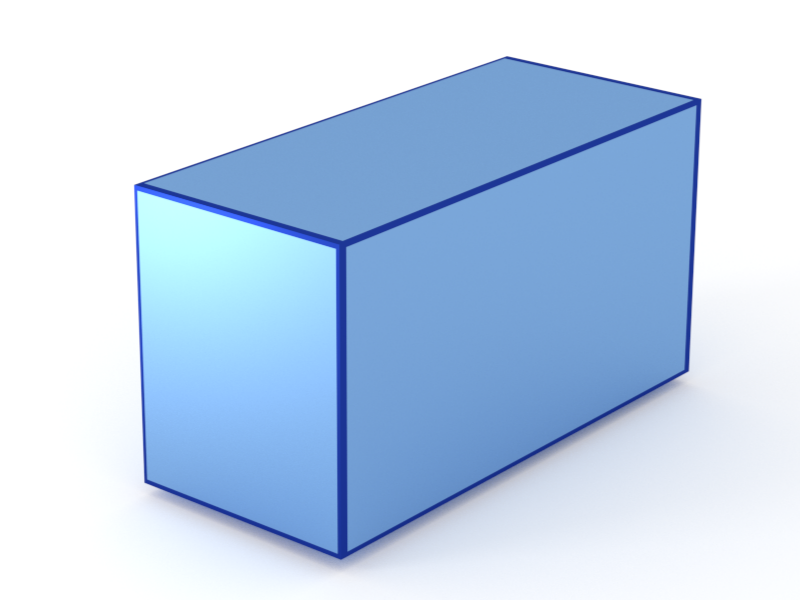
\includegraphics[width=1in]{fig/blue/Box3d.png} & & 
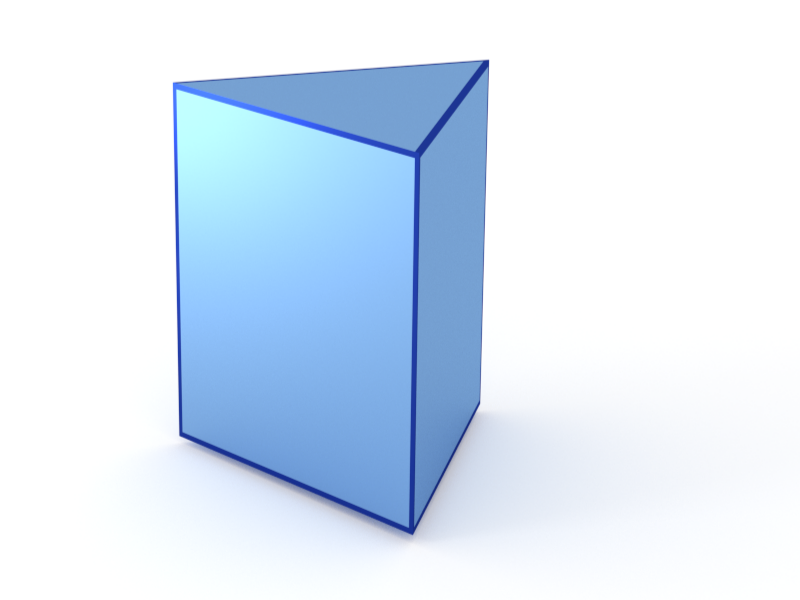
\includegraphics[width=1in]{fig/blue/Prism33d.png} & & 
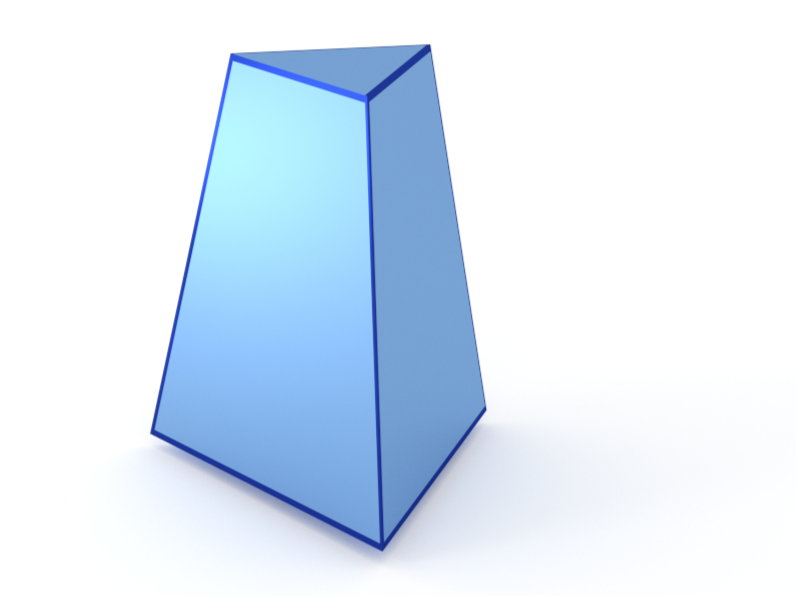
\includegraphics[width=1in]{fig/blue/Tetrahedron3d.png} & & 
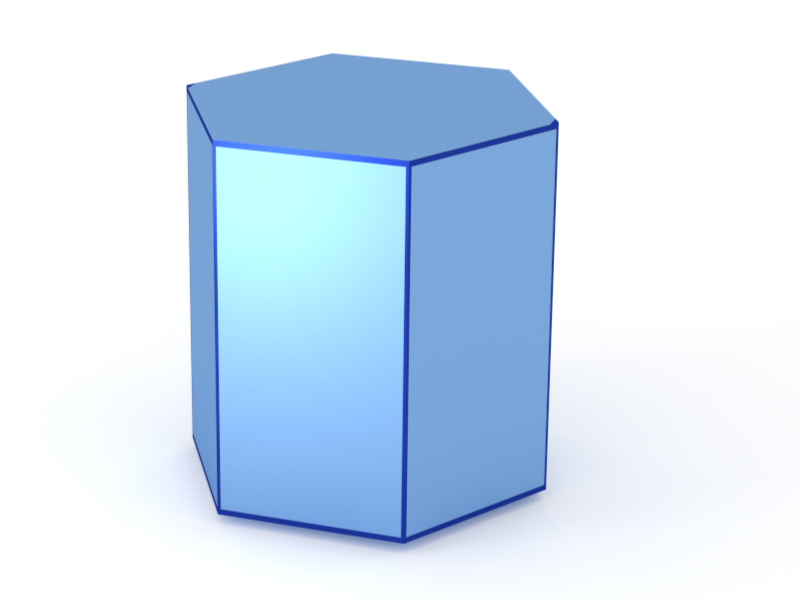
\includegraphics[width=1in]{fig/blue/Prism63d.png} 
\\
\hline 
Cone6,  Sect.~\ref{sec:Cone6} & &  Pyramid, Sect.~\ref{sec:Pyramid} & & Anisotropic pyramid,  Sect.~\ref{sec:AnisoPyramid} & &  {Cuboctahedron}, Sect.~\ref{sec:Cuboctahedron}\\
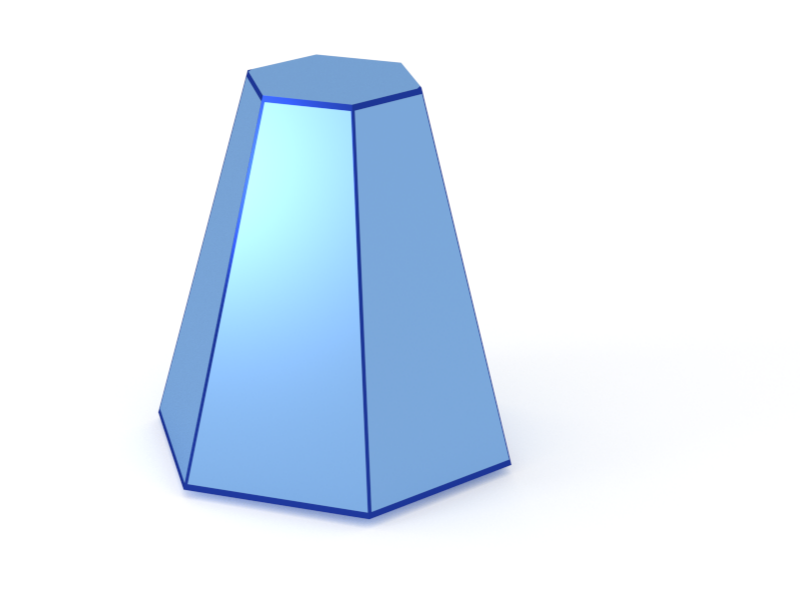
\includegraphics[width=1in]{fig/blue/Cone63d.png}  & & 
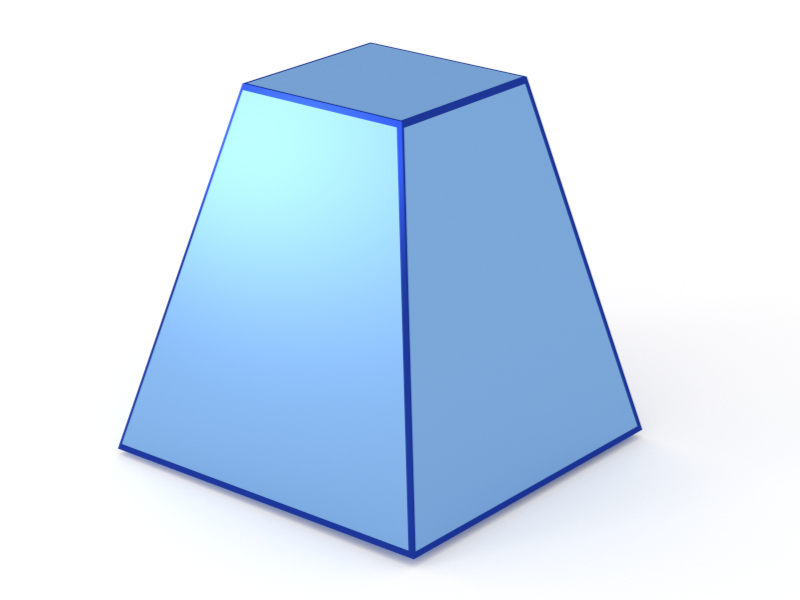
\includegraphics[width=1in]{fig/blue/Pyramid3d.png} & &
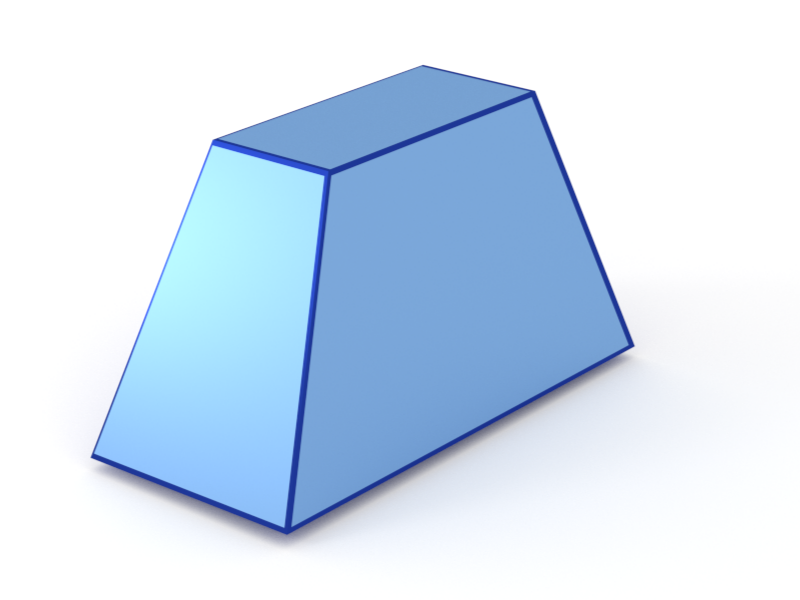
\includegraphics[width=1in]{fig/blue/AnistropicPyramid3d.png} & & 
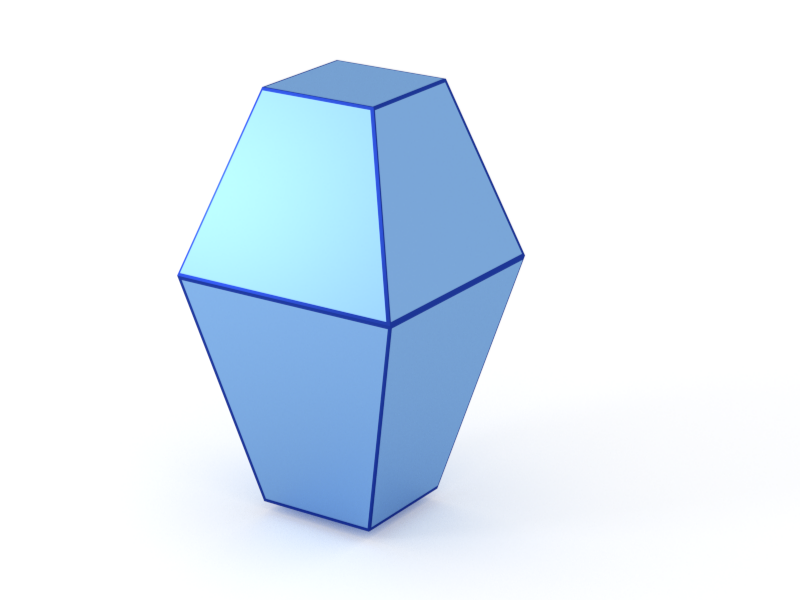
\includegraphics[width=1in]{fig/blue/Cuboctahedron3d.png}
\\
\hline
Cylinder, Sect.~\ref{sec:Cylinder}  & & Ellipsoidal cylinder, Sect.~\ref{sec:EllipsoidalCylinder} & &  Cone,\phantom{--} Sect.~\ref{sec:Cone} & & Full Sphere, Sect.~\ref{sec:FullSphere} \\

\includegraphics[width=1in]{fig/blue/Cylinder3d.png} & & 
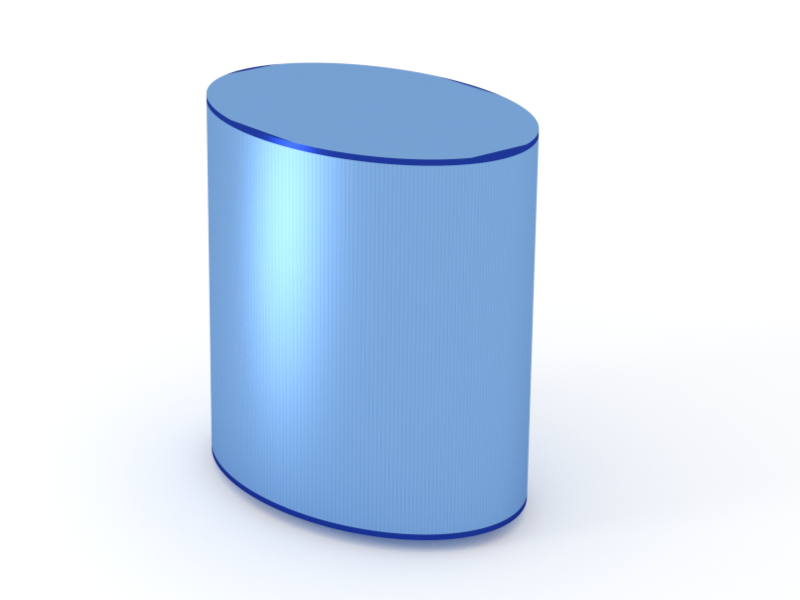
\includegraphics[width=1in]{fig/blue/EllipsoidalCylinder3d.png} & & 
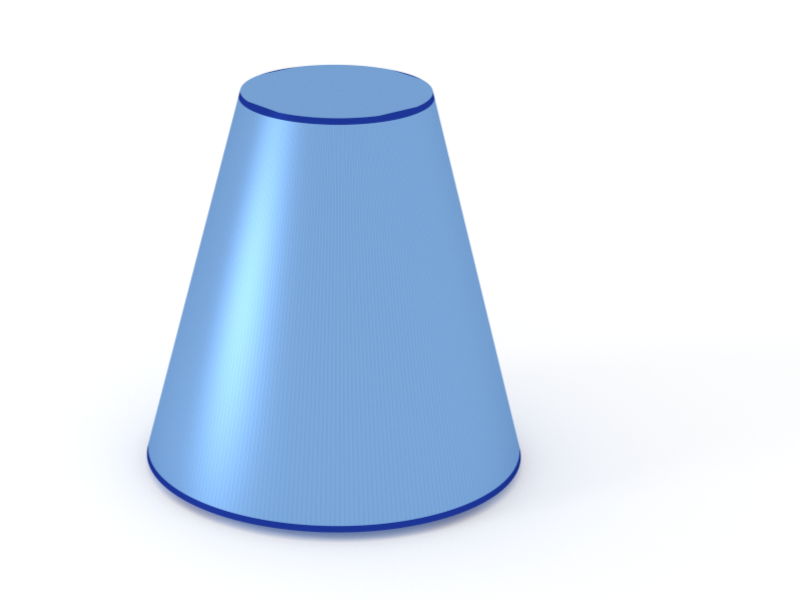
\includegraphics[width=1in]{fig/blue/Cone3d.png} & & 
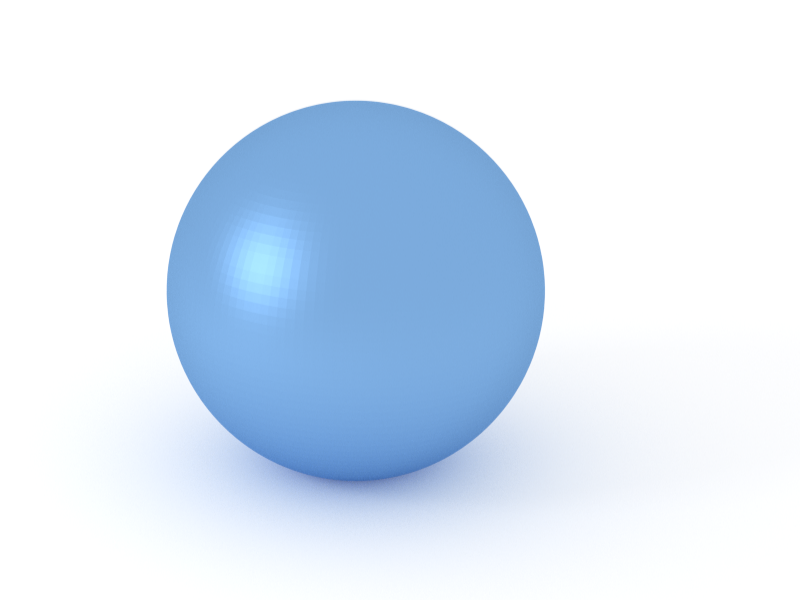
\includegraphics[width=1in]{fig/blue/FullSphere3d.png} \\
\hline
Truncated Sphere, Sect.~\ref{sec:Sphere}  & & Full Spheroid, Sect.~\ref{sec:FullSpheroid} & & Truncated Spheroid,  Sect.~\ref{sec:Spheroid} & & Hemi Ellipsoid, Sect.~\ref{sec:HemiEllipsoid}\\
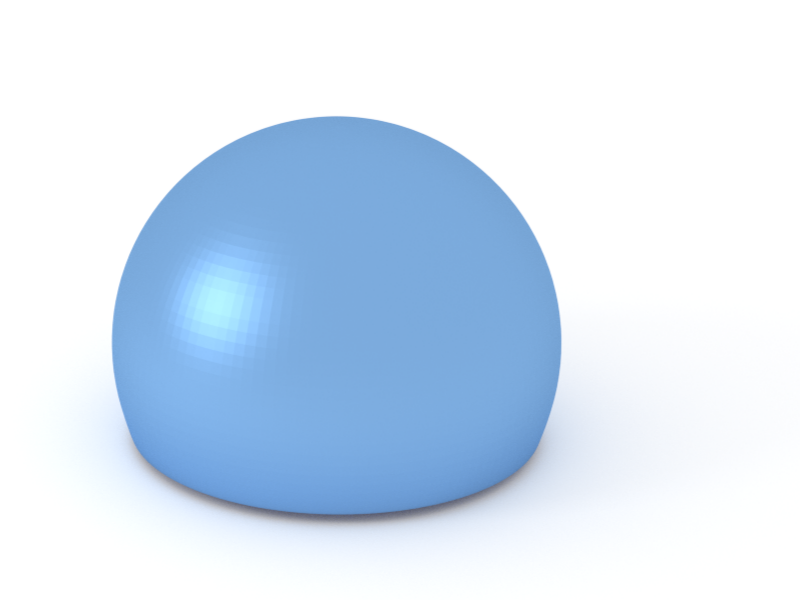
\includegraphics[width=1in]{fig/blue/Sphere3d.png}  & & 
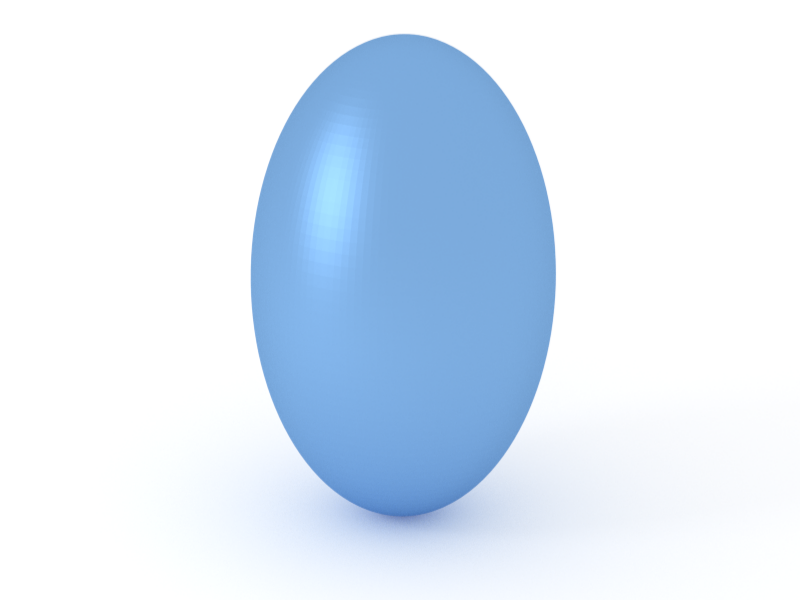
\includegraphics[width=1in]{fig/blue/FullSpheroid3d.png} & & 
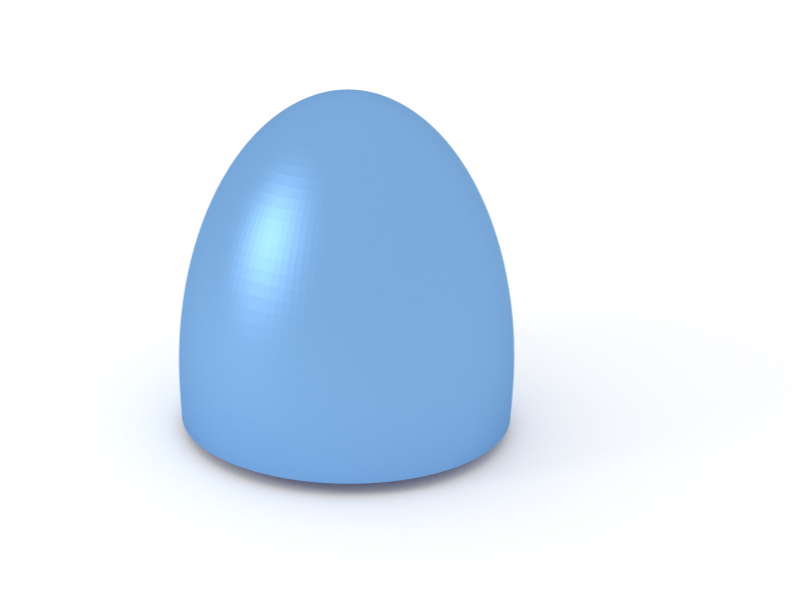
\includegraphics[width=1in]{fig/blue/Spheroid3d.png} & & 
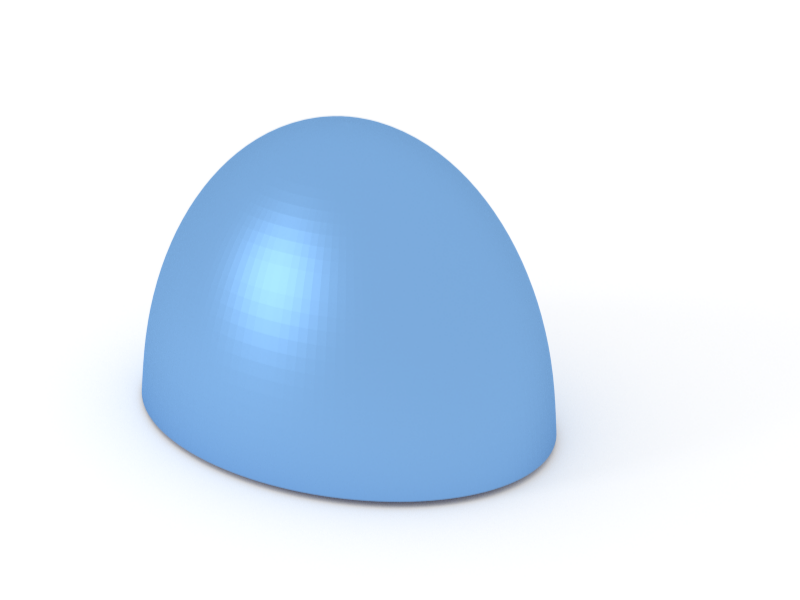
\includegraphics[width=1in]{fig/blue/HemiEllipsoid3d.png}\\
\hline
Ripple1, Sect.~\ref{sec:Ripple1} &  & Ripple2, Sect.~\ref{sec:Ripple2}&  & Truncated cube Sect.~\ref{sec:Truncatedcube} & &  \\
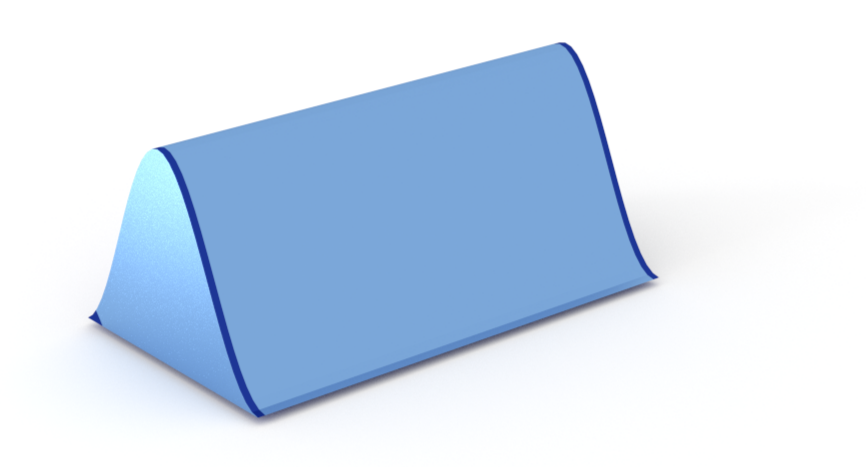
\includegraphics[width=1in]{fig/blue/Ripple13d.png} & & 
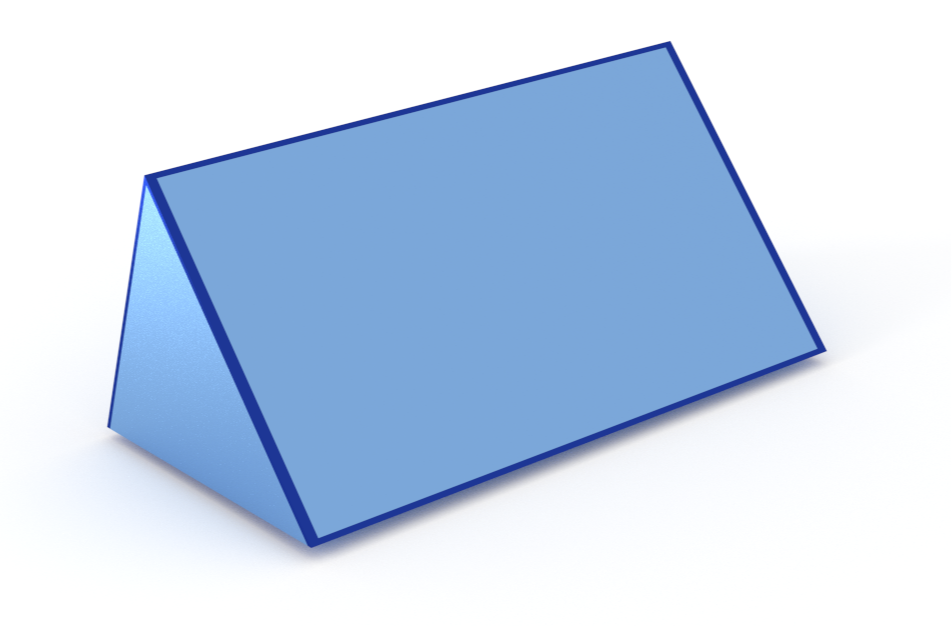
\includegraphics[width=1in]{fig/blue/Ripple23d.png} & &  
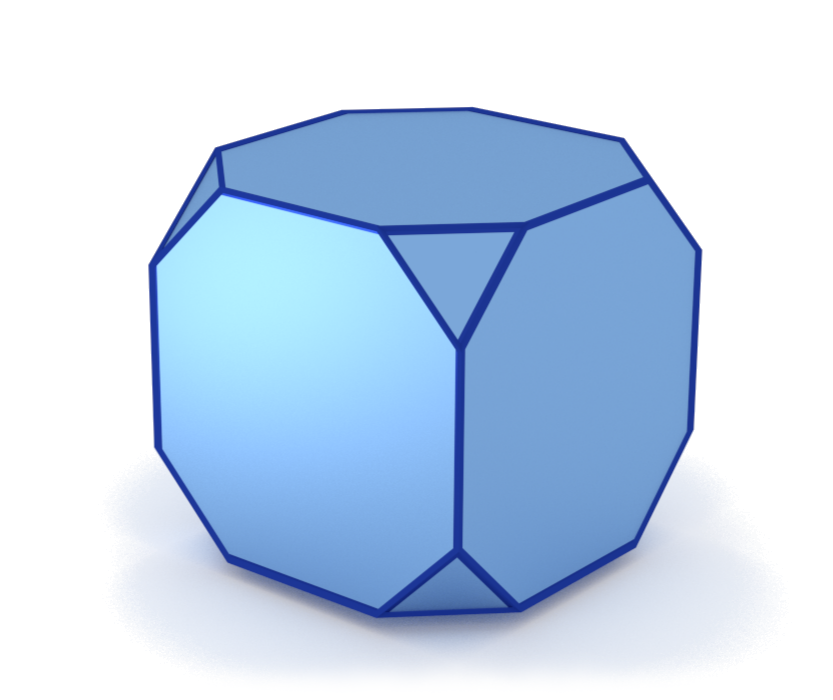
\includegraphics[width=.75in]{fig/blue/TruncatedCube3d.png}
& & \\
\hline 
\end{tabulary}
\caption{Table of form factors implemented in \BornAgain.} \label{tab:formfactors}
\index{Form factor!table of implemented models}
\end{table}

\FloatBarrier

%-------------------------------------------------------------------------------
\newpage
\ifodd\value{page}\textit{Page intentionally left blank}\newpage\fi
\subsection{Box (cuboid)} \label{sec:Box}
  \index{Box (form factor)}
  \index{Cuboid (form factor)}
  \index{Prism (form factor)!reactangular (Box)}
  \index{FormFactorBox@\Code{FormFactorBox}}
%-------------------------------------------------------------------------------

\paragraph{Real-space geometry}\strut\\
A rectangular cuboid, as shown in fig.~\ref{fig:box}. 

\begin{figure}[ht]
\hfill
\subfigure[Side view]{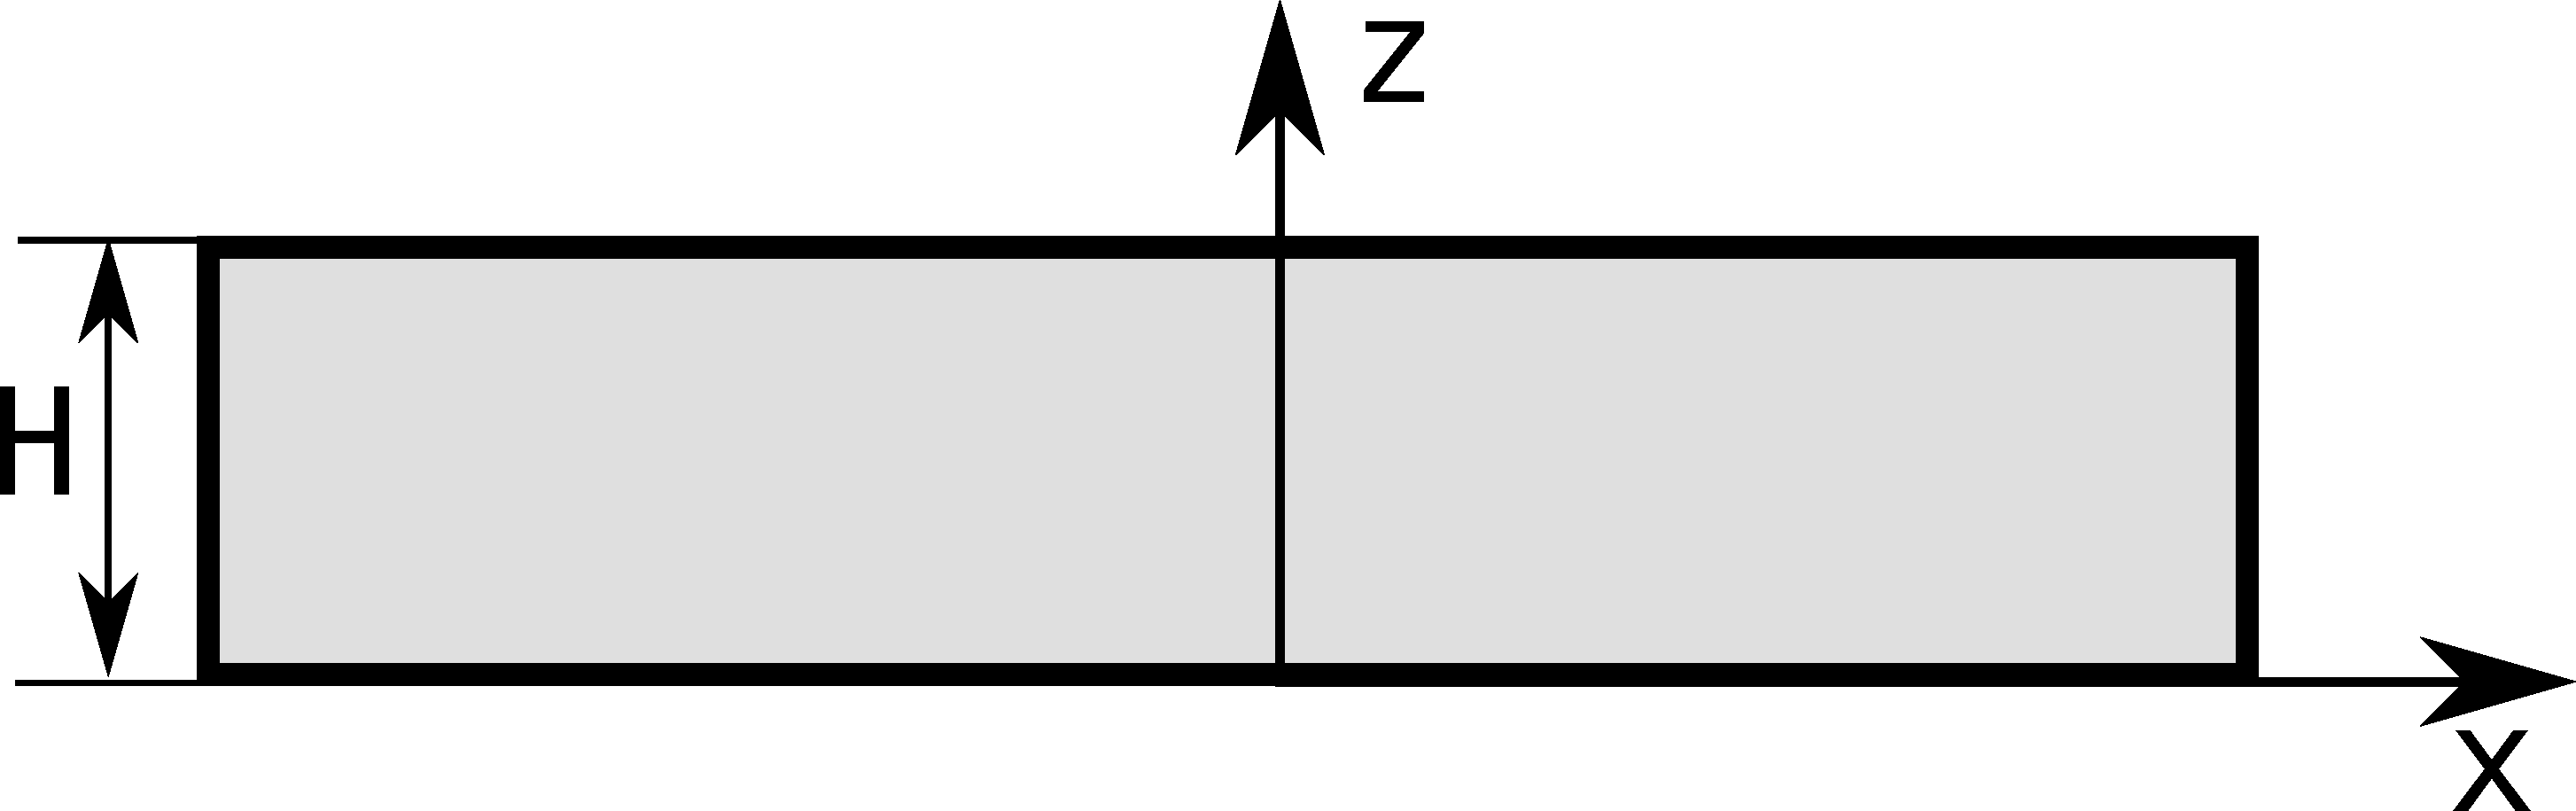
\includegraphics[width=5cm]{fig/cuts/Box2dxz.pdf}}
\hfill
\subfigure[Top view]{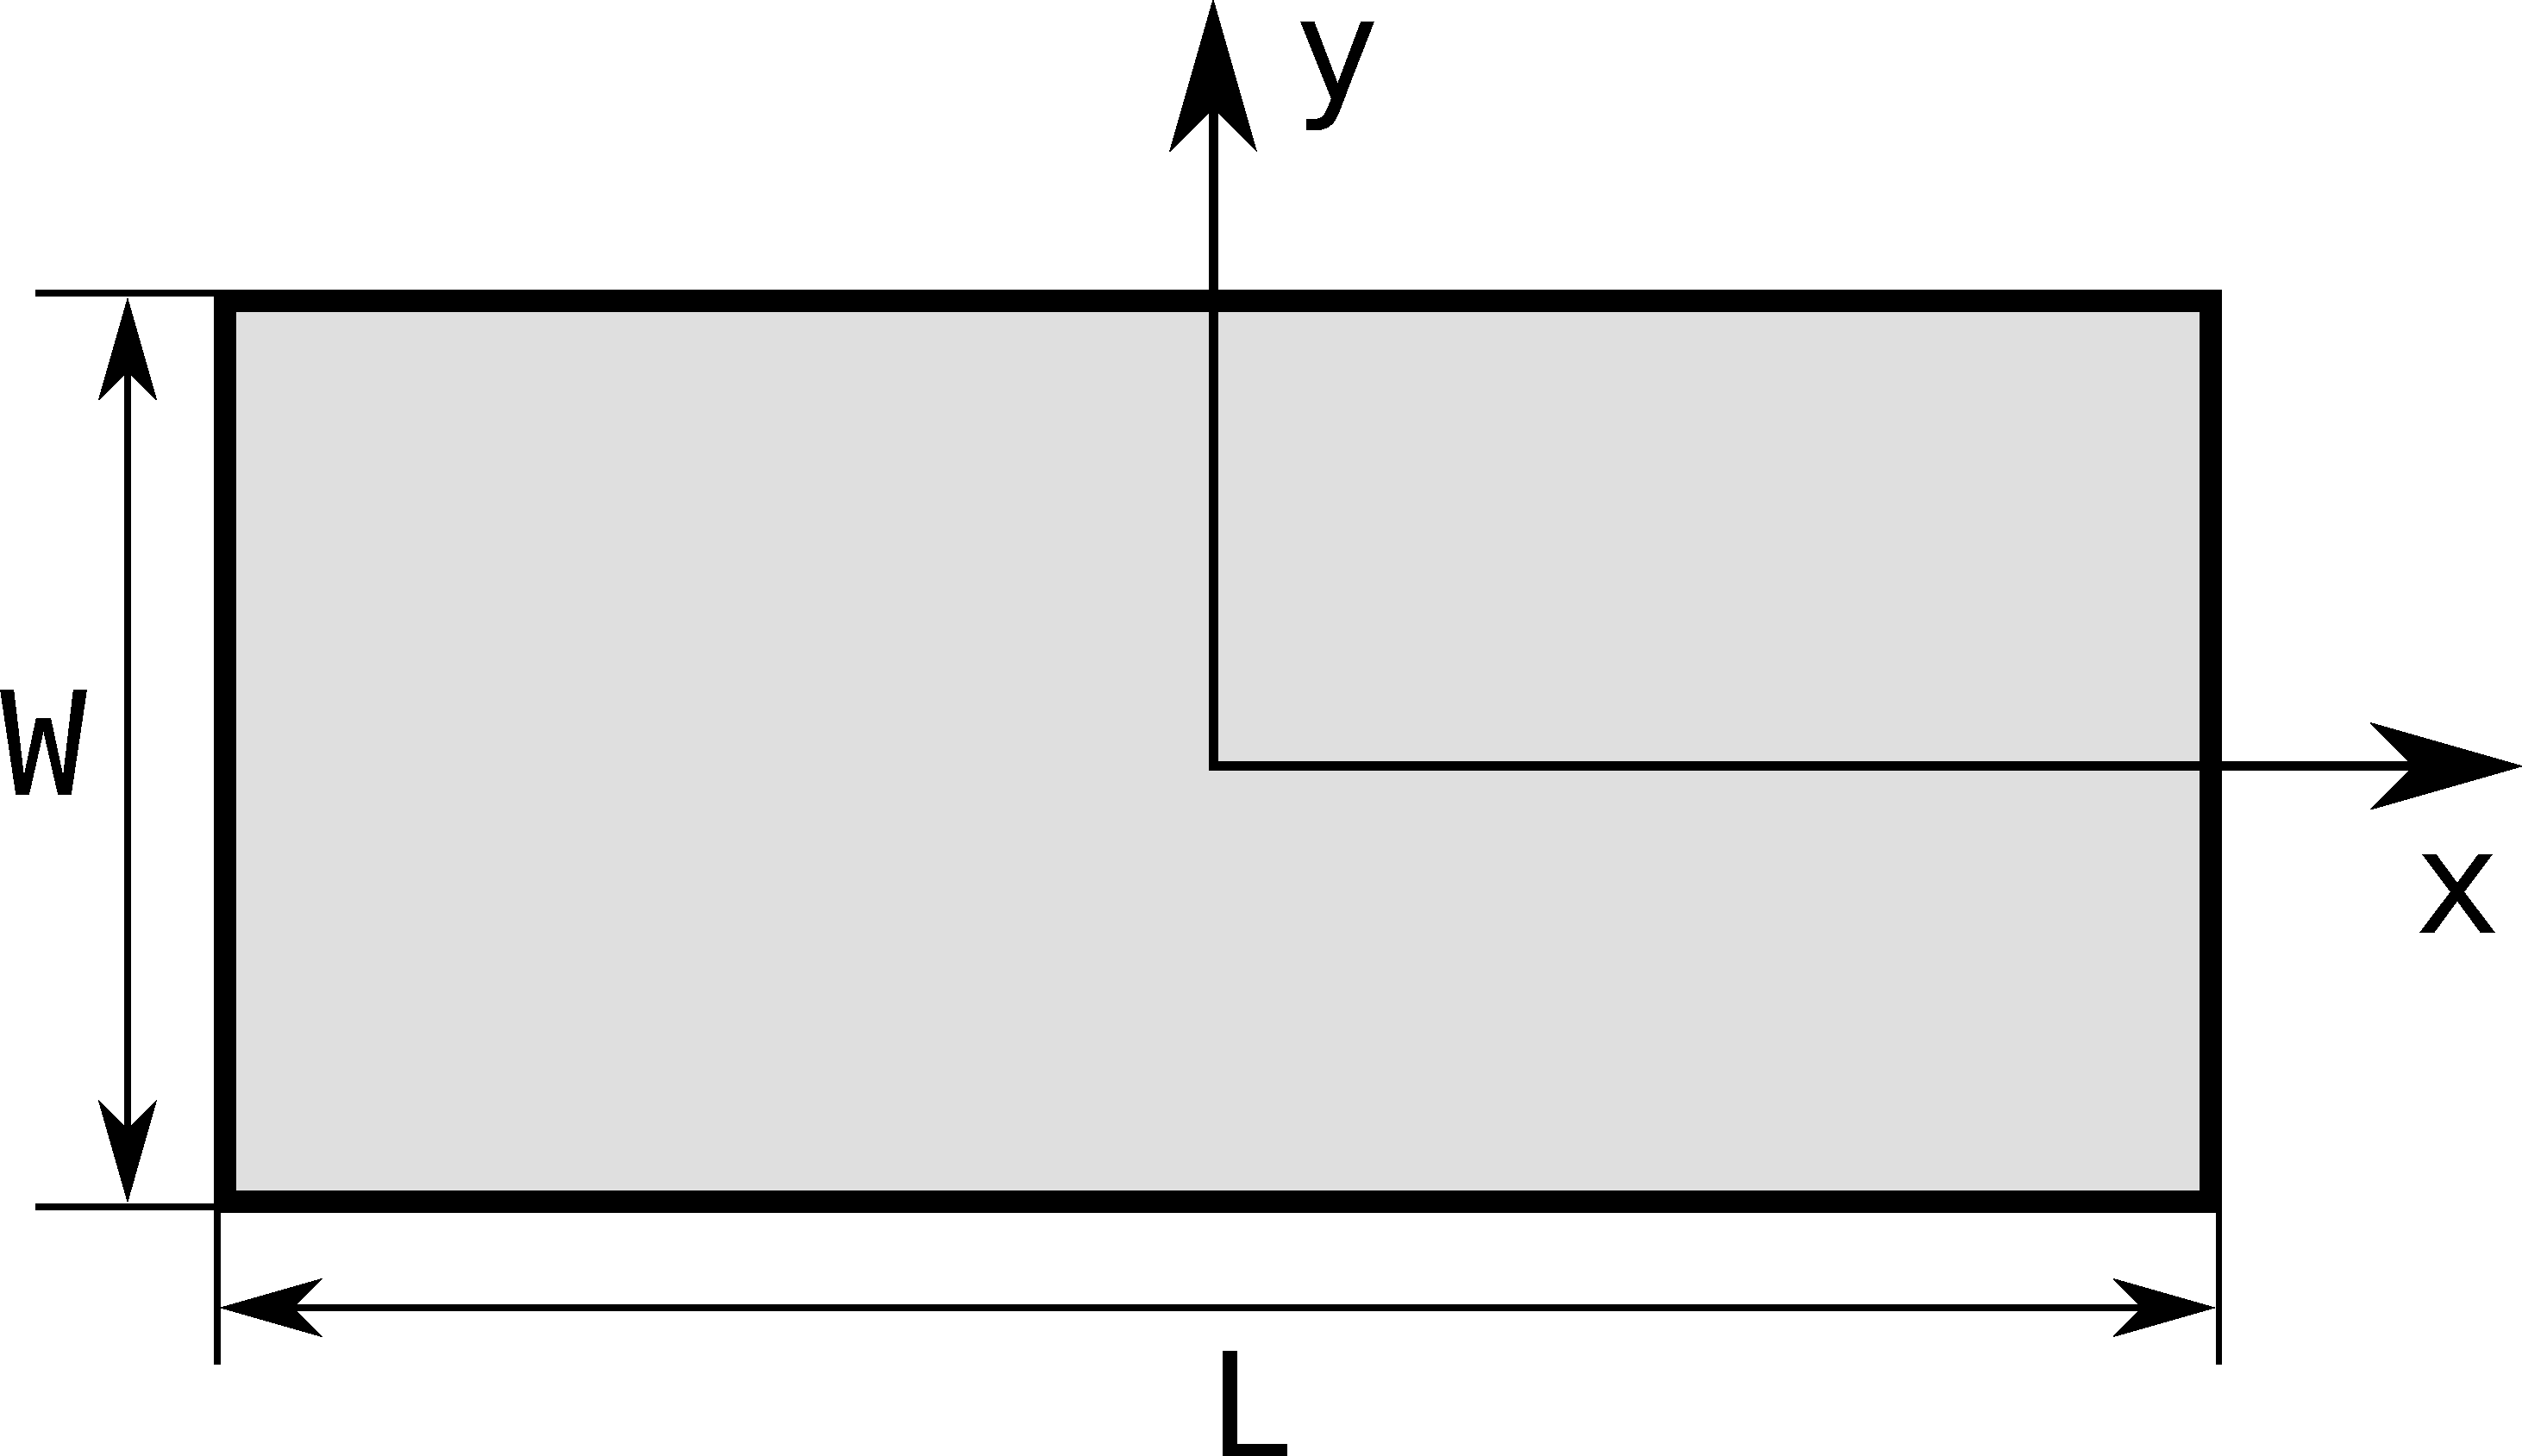
\includegraphics[width=5cm]{fig/cuts/Box2dxy.pdf}}
\hfill
\caption{Sketch of a Box.}
\label{fig:box}
\end{figure}

\FloatBarrier

\paragraph{Parameters}
\begin{itemize}
\item length of the base $L$,
\item width of the base $W$,
\item height  $H$.
\end{itemize}

\paragraph{Properties}
\begin{itemize}
\item volume $V= LWH$,
\item particle surface seen from above $S = LW$.
%\item radius of gyration
\end{itemize}

\paragraph{Form factor}

\begin{equation*}
F(\mathbf{q},L,W,H)= L W H\exp\left(i q_z \frac{H}{2}\right) \sinc\left(q_x \frac{L}{2}\right)
\sinc\left(q_y \frac{W}{2}\right) \sinc\left(q_z \frac{H}{2}\right),
\end{equation*}
where $\sinc(x)=\sin(x)/x$ is the cardinal sine.

\paragraph{Syntax}\strut\\
\Code{FormFactorBox(length, width, height)}

\newpage

\paragraph{Example}\strut\\
Figure~\ref{fig:FFBoxEx} shows the normalized intensity
$|F|^2/V^2$, computed with $L=20$~nm, $W=16$~nm, and $H=13$~nm:

\begin{figure}[ht]
\begin{center}
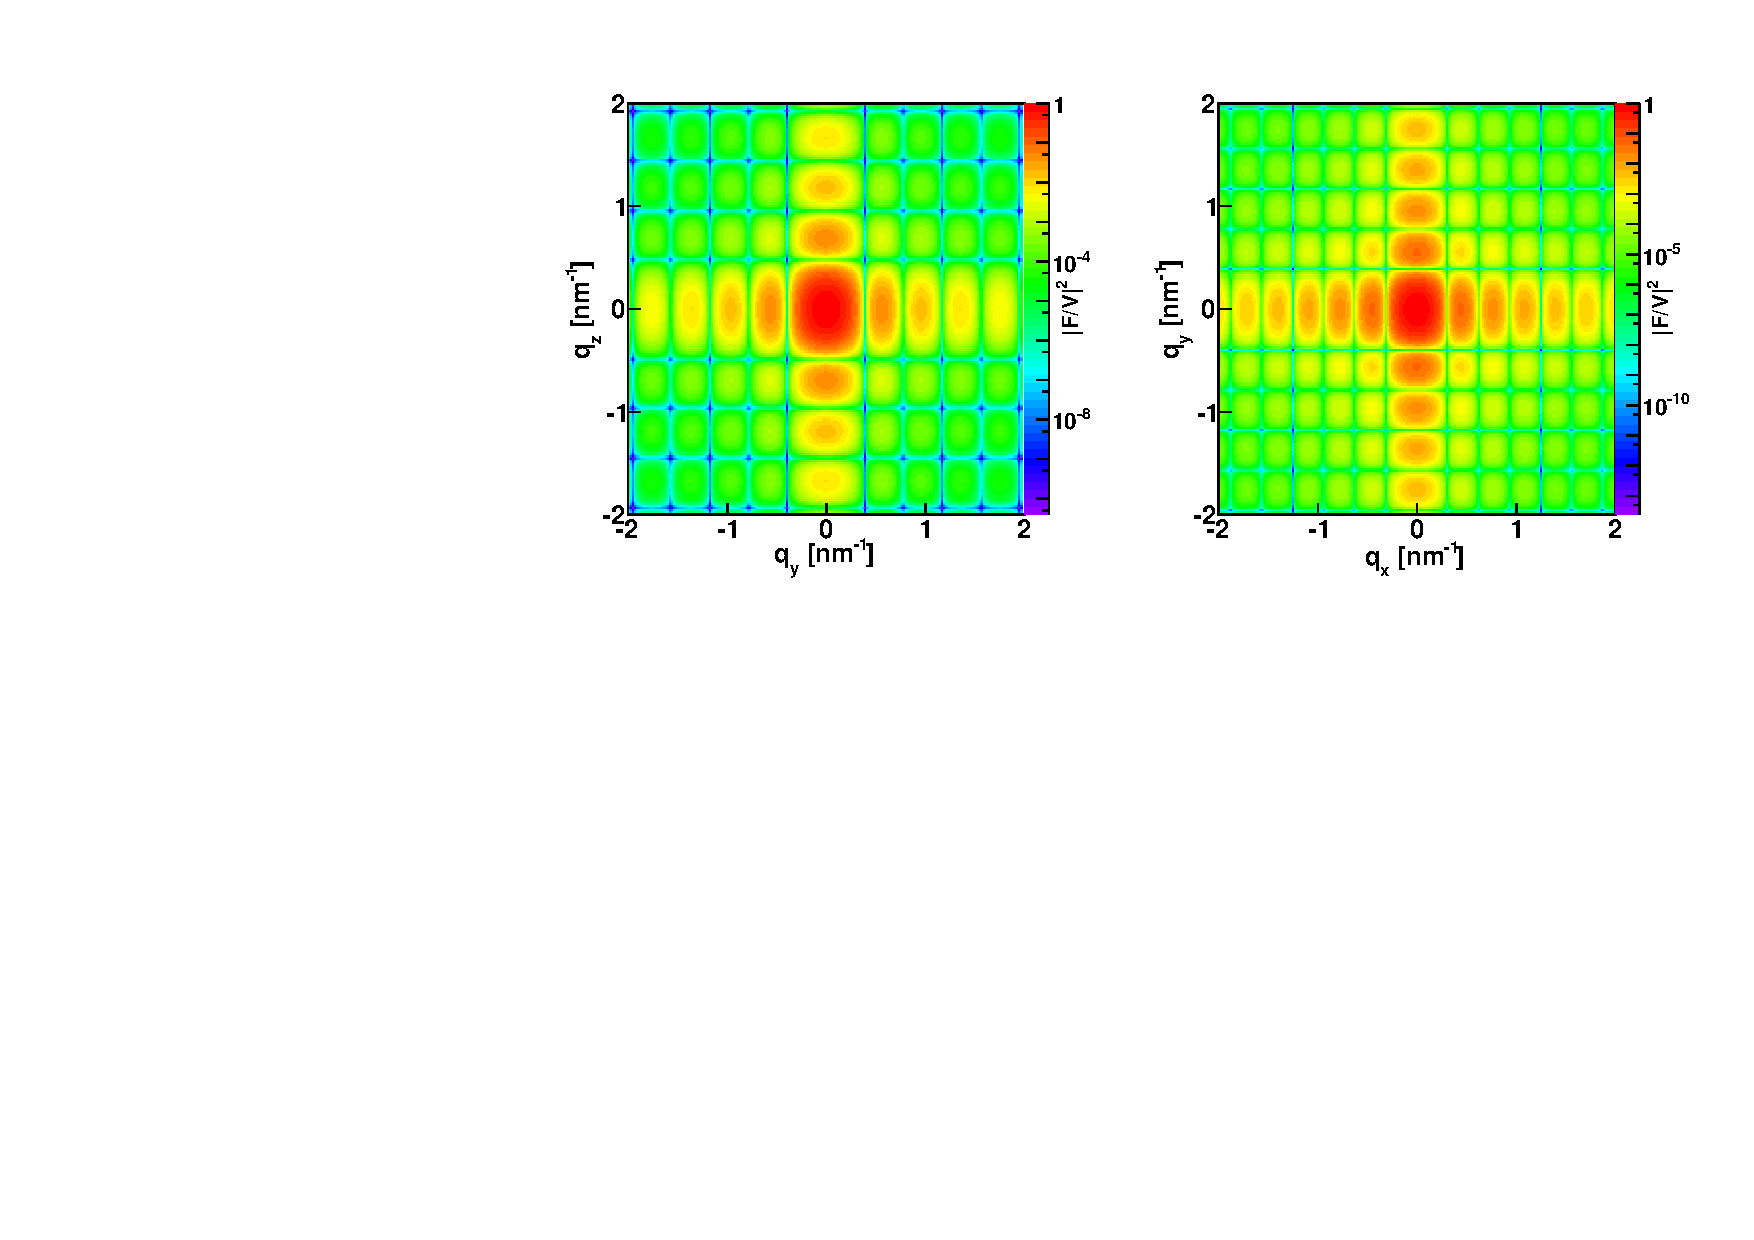
\includegraphics[angle=-90,width=\textwidth]{fig/ff/figffbox.pdf}
\end{center}
\caption{Normalized intensity for the form factor of a Box plotted against ($q_y$, $q_z$) and  ($q_x$, $q_y$) and computed with \Code{FormFactorBox(20.*nanometer, 16.*nanometer, 13.*nanometer)}.}
\label{fig:FFBoxEx}
\end{figure}

\paragraph{References}\strut\\
Agrees with \lq\lq Box\rq\rq\ form factor of \IsGISAXS~\cite{Laz02},
except for factors $1/2$ in the definitions of parameters $L$, $W$, $H$.

%-------------------------------------------------------------------------------
\newpage
\subsection{Prism3 (triangular)} \label{sec:Prism3}
  \index{Prism (form factor)!triangular (Prism3)}
  \index{FormFactorPrism3@\Code{FormFactorPrism3}}
%-------------------------------------------------------------------------------

\paragraph{Real-space geometry}\strut\\
A triangular prism, whose base is an equilateral
triangle, as shown in fig.~\ref{fig:prism3}.

\begin{figure}[ht]
\hfill
\subfigure[Side view]{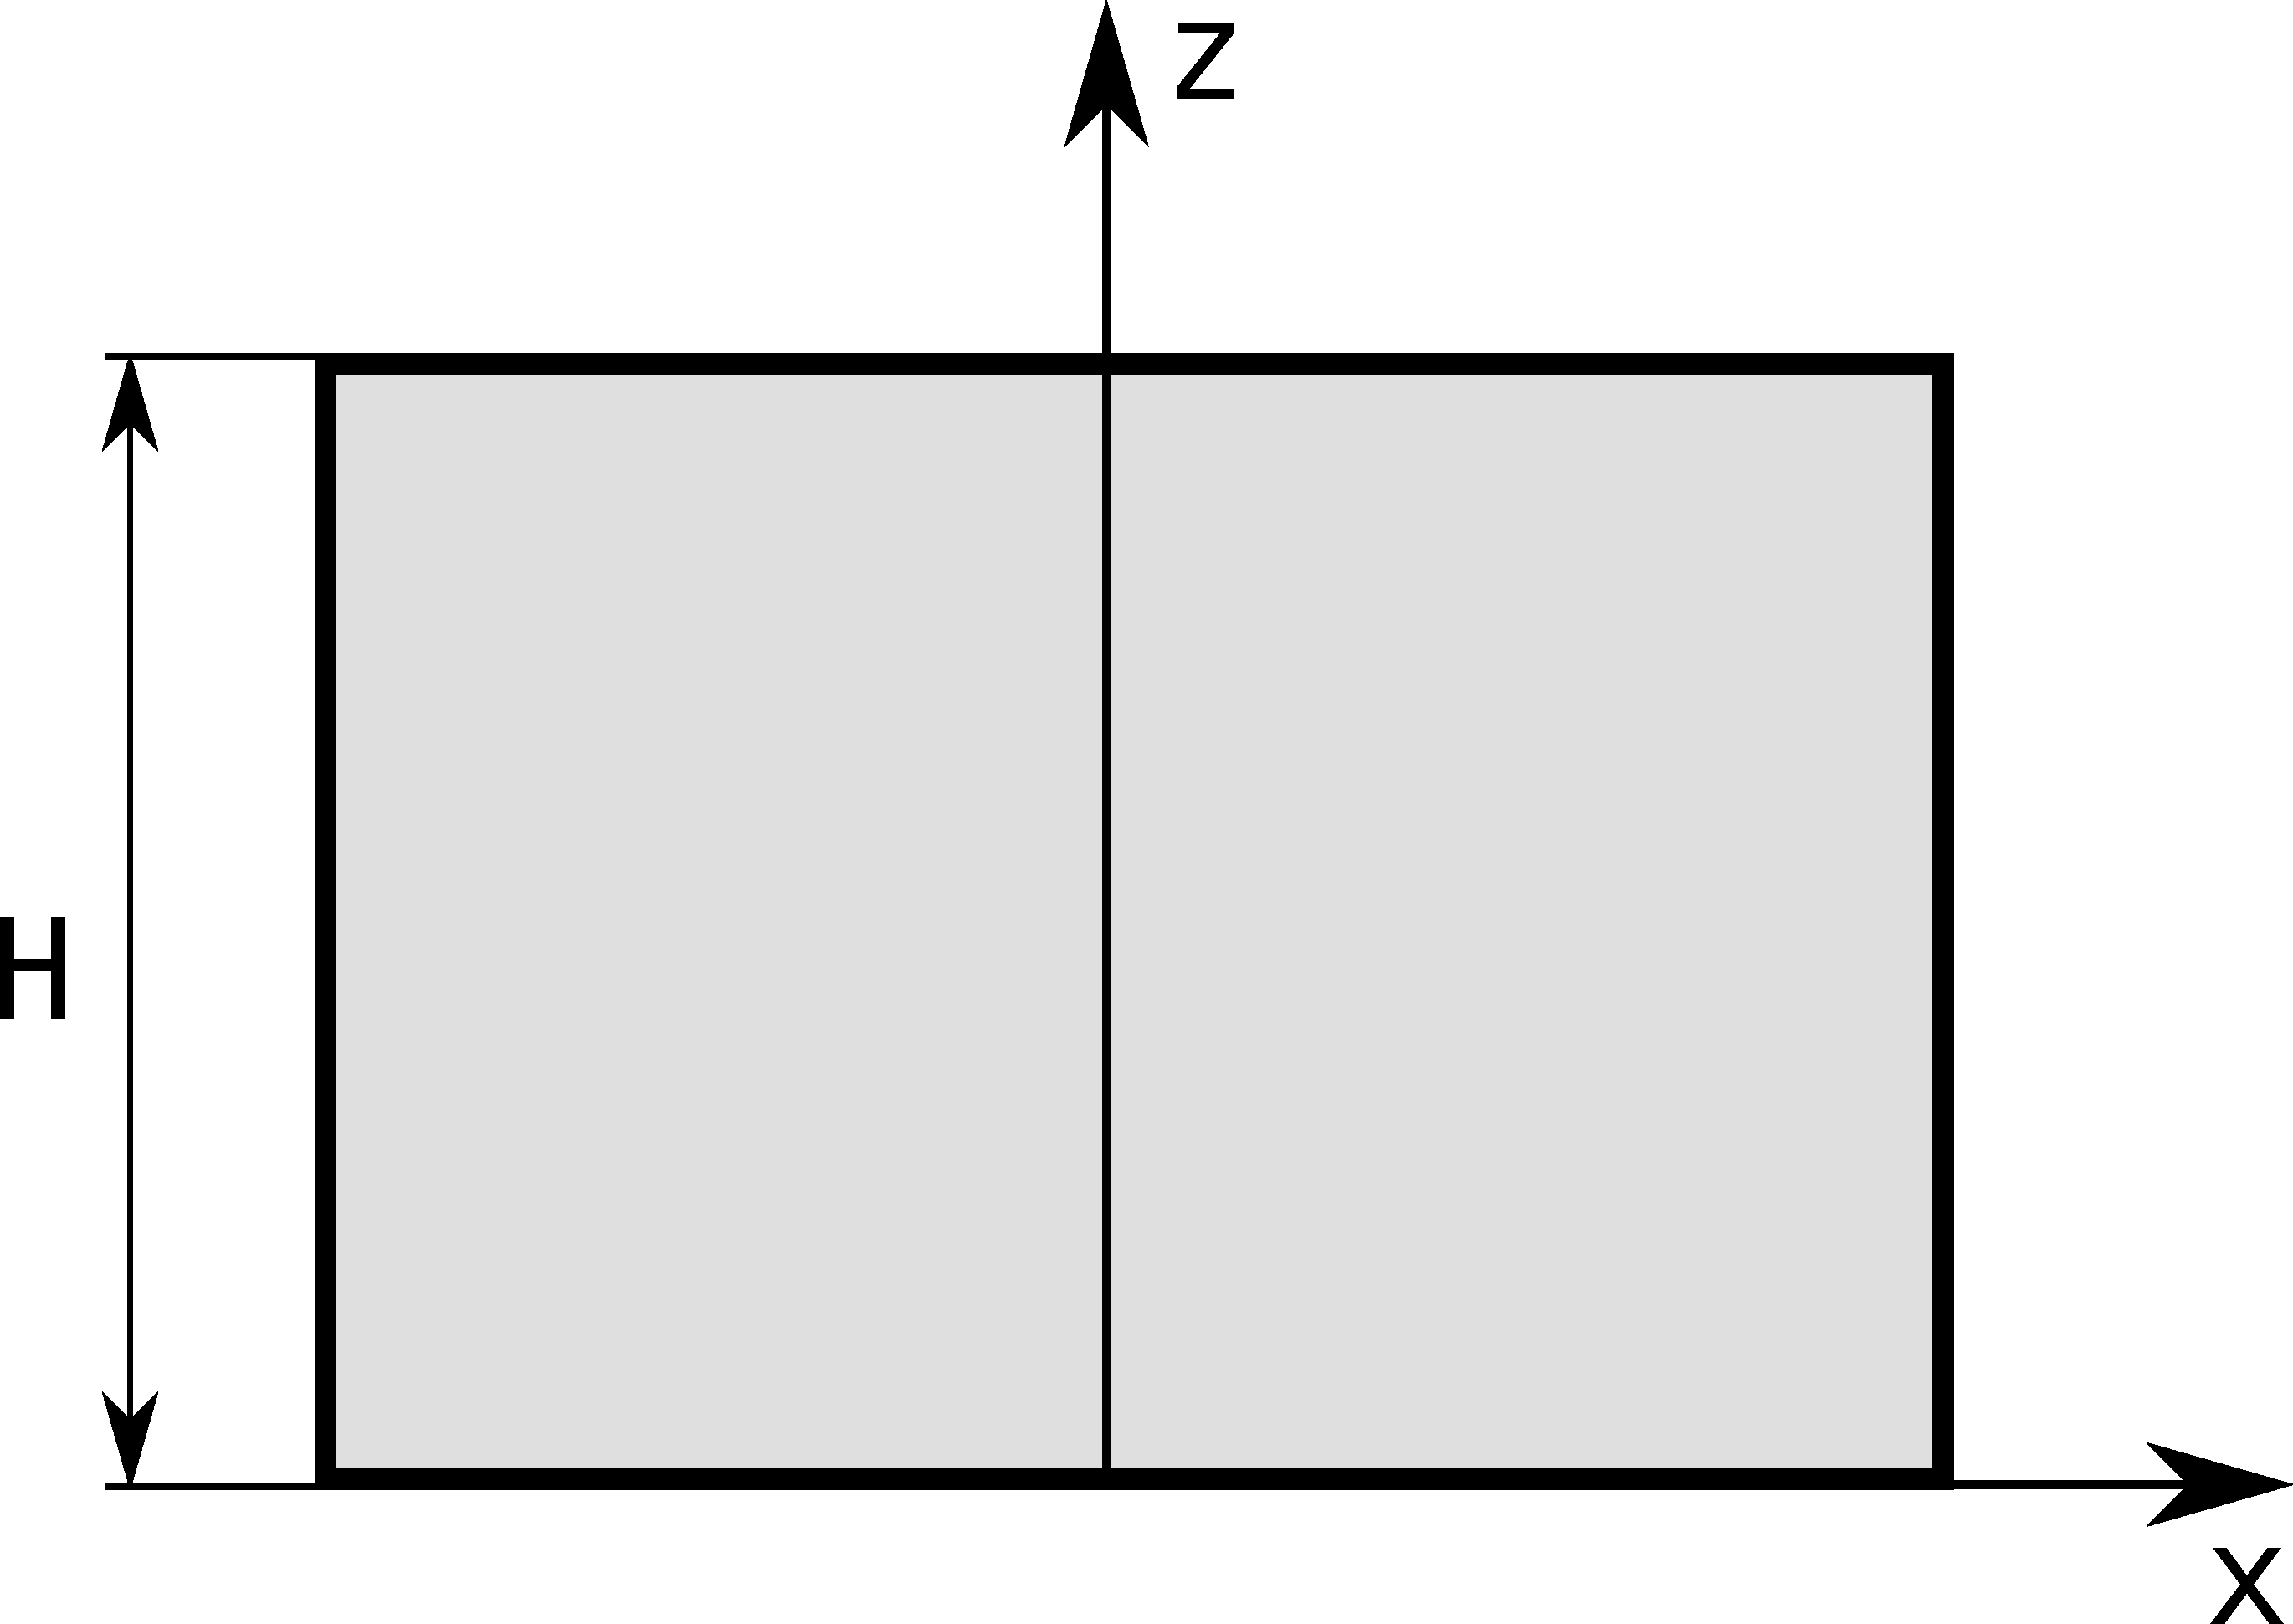
\includegraphics[width=5cm]{fig/cuts/Prism32dxz.pdf}}
\hfill
\subfigure[Top view]{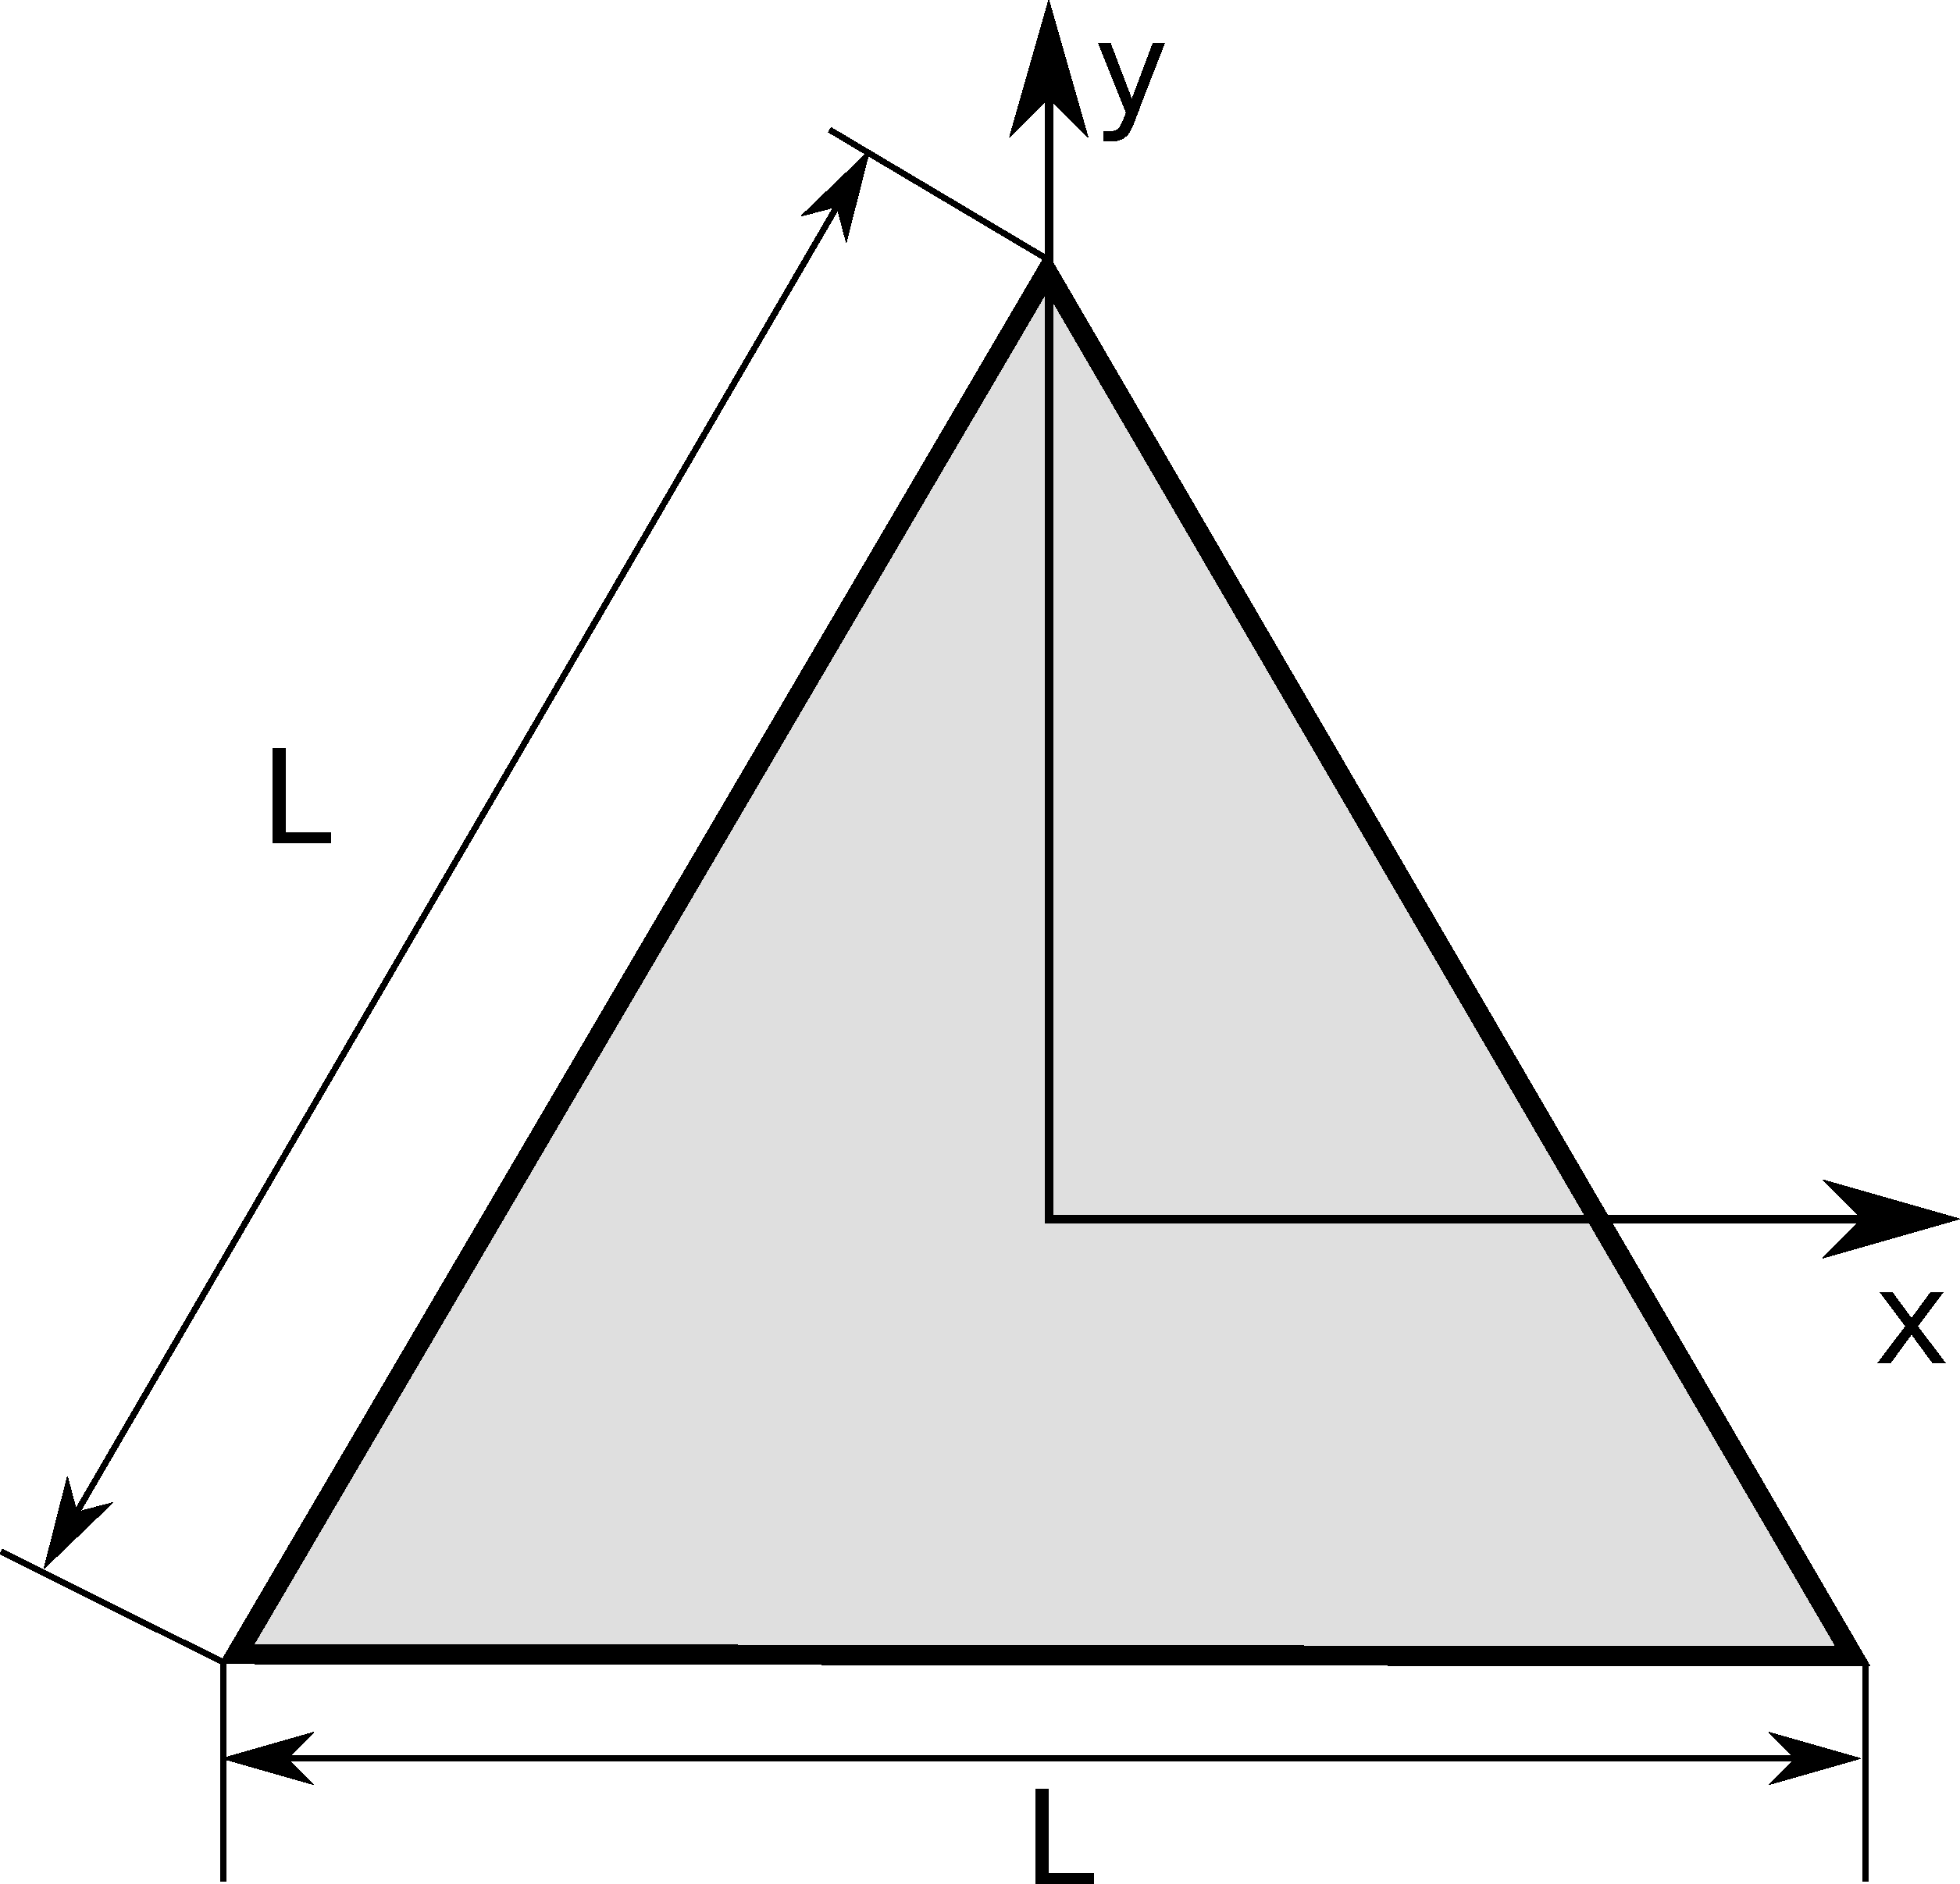
\includegraphics[width=5cm]{fig/cuts/Prism32dxy.pdf}}
\hfill
\caption{Sketch of a Prism3.}
\label{fig:prism3}
\end{figure}

\FloatBarrier

\paragraph{Parameters}
\begin{itemize}
\item length $L$ of one side of the base, 
\item height $H$.
\end{itemize}

\paragraph{Properties}
\begin{itemize}
\item volume $V= \dfrac{\sqrt{3}}{4} H L^2$,
\item particle surface seen from above $S =\dfrac{\sqrt{3}}{4}L^2$.

\end{itemize}

\paragraph{Form factor}
\begin{align*}
F(\mathbf{q},L, H) &= \frac{2 \sqrt{3}}{q_x^2-3q_y^2}  \exp\left(-i q_y\frac{L}{2\sqrt{3}}\right)\left[\exp\left(i \sqrt{3} q_y \frac{L}{2} \right)-\cos\left(q_x \frac{L}{2}\right)-i \sqrt{3} q_y \frac{L}{2} \sinc\left(q_x \frac{L}{2}\right) \right] \\
  &
\times  H \sinc\left(q_z \frac{H}{2} \right) \exp\left(i q_z \frac{H}{2}\right),
\end{align*}
where $\sinc(x)=\sin(x)/x$ is the cardinal sine.

\paragraph{Syntax}\strut\\
\Code{FormFactorPrism3(length, height)}

\paragraph{Example}\strut\\
Figure~\ref{fig:FFprism3Ex} shows the normalized intensity
$|F|^2/V^2$, computed with $L=10$~nm and \mbox{$H=13$~nm.}
\begin{figure}[ht]
\begin{center}
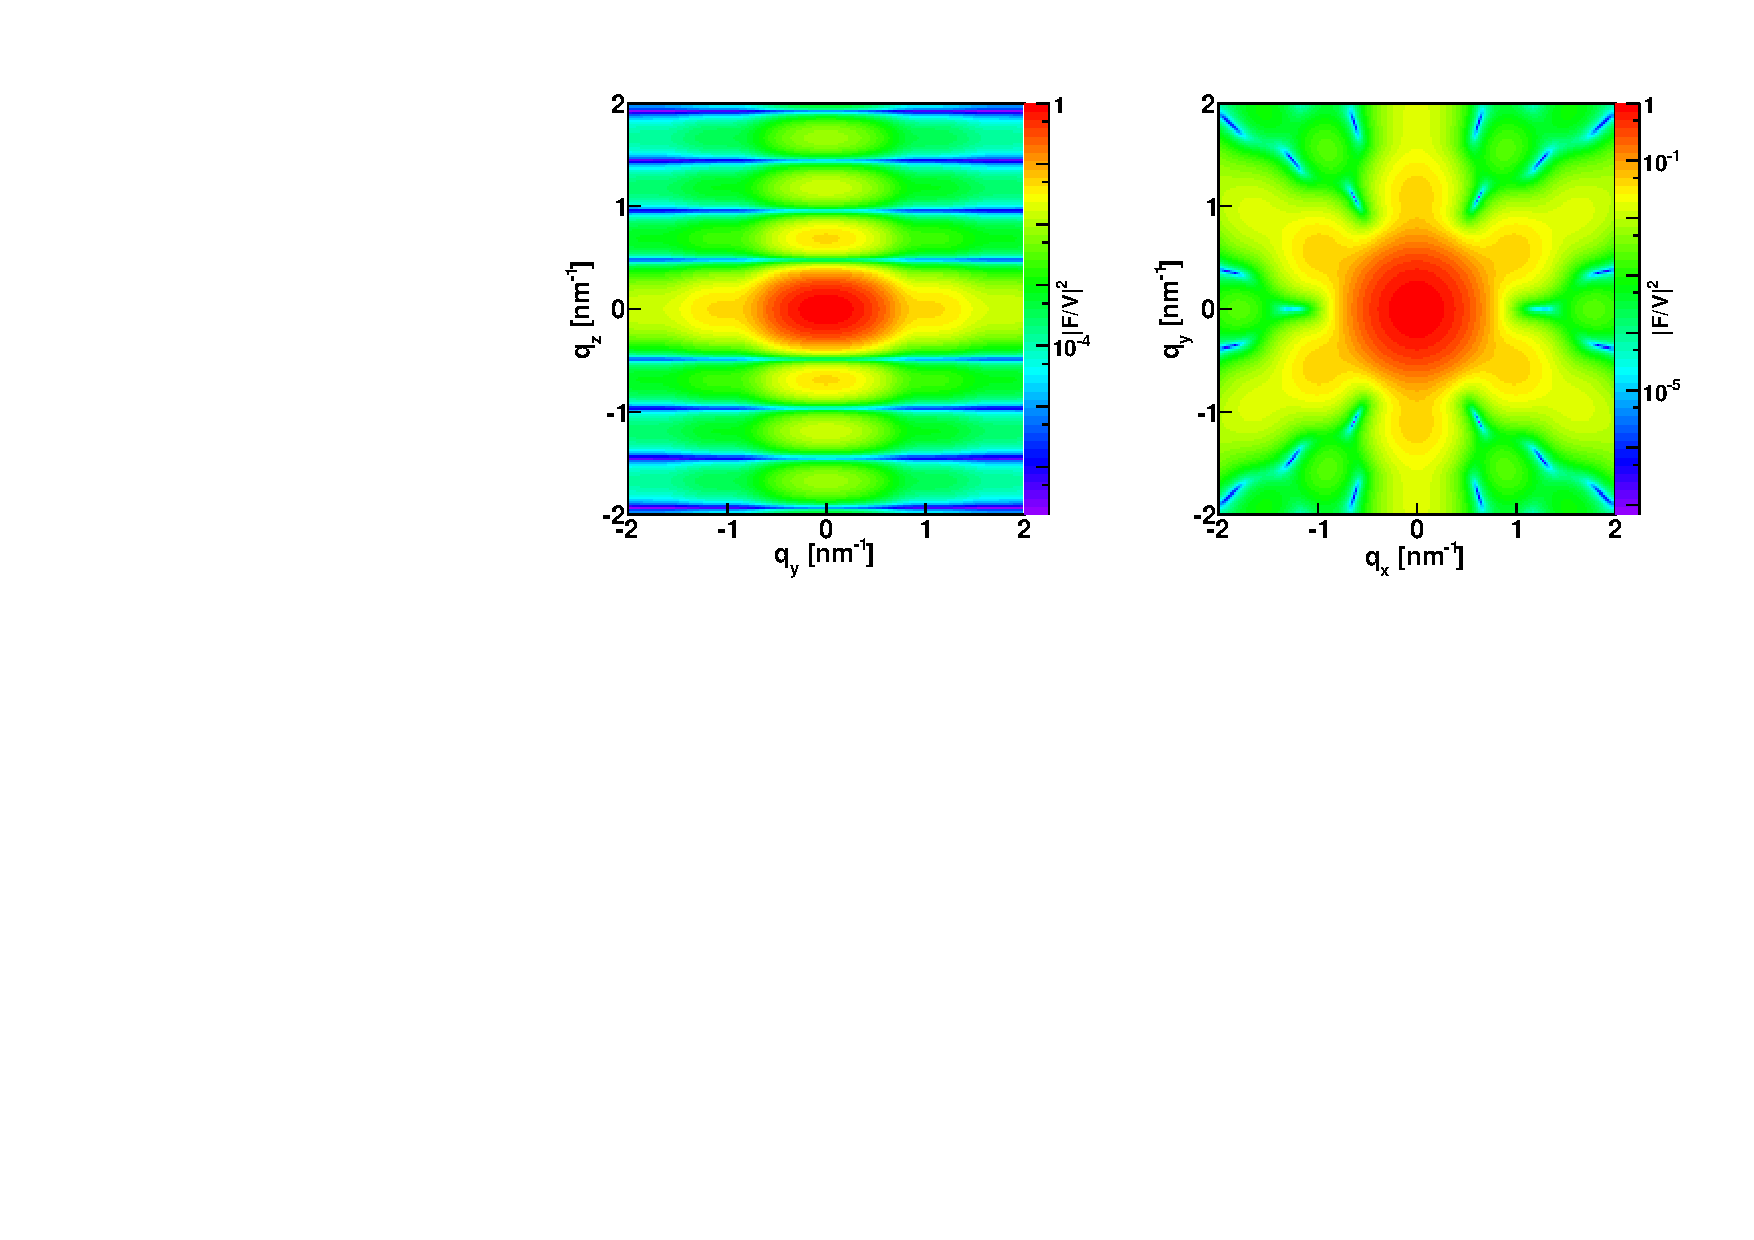
\includegraphics[angle=-90,width=\textwidth]{fig/ff/figffprism3.pdf}
\end{center}
\caption{Normalized intensity for the form factor of a Prism3
 plotted against ($q_y$, $q_z$) and  ($q_x$, $q_y$) and
  computed with \Code{FormFactorPrism3(10.*nanometer, 13.*nanometer)}.}
\label{fig:FFprism3Ex}
\end{figure}

\paragraph{References}\strut\\
Agrees with \lq\lq Prism3\rq\rq\ form factor of \IsGISAXS~\cite{Laz02},
except for the definition of parameter $L= 2 R_{\rm{\Code{IsGISAXS}}}$.

%-------------------------------------------------------------------------------
\newpage
\subsection{Tetrahedron} \label{sec:Tetrahedron}
  \index{Tetrahedron (form factor)}
  \index{Truncated tetrahedron (form factor)}
  \index{FormFactorTetrahedron@\Code{FormFactorTetrahedron}}
%-------------------------------------------------------------------------------
 
\paragraph{Real-space geometry}\strut\\
A truncated tetrahedron as shown in fig.~\ref{fig:tetrahedron}.

\begin{figure}[ht]
\hfill
\subfigure[Side view]{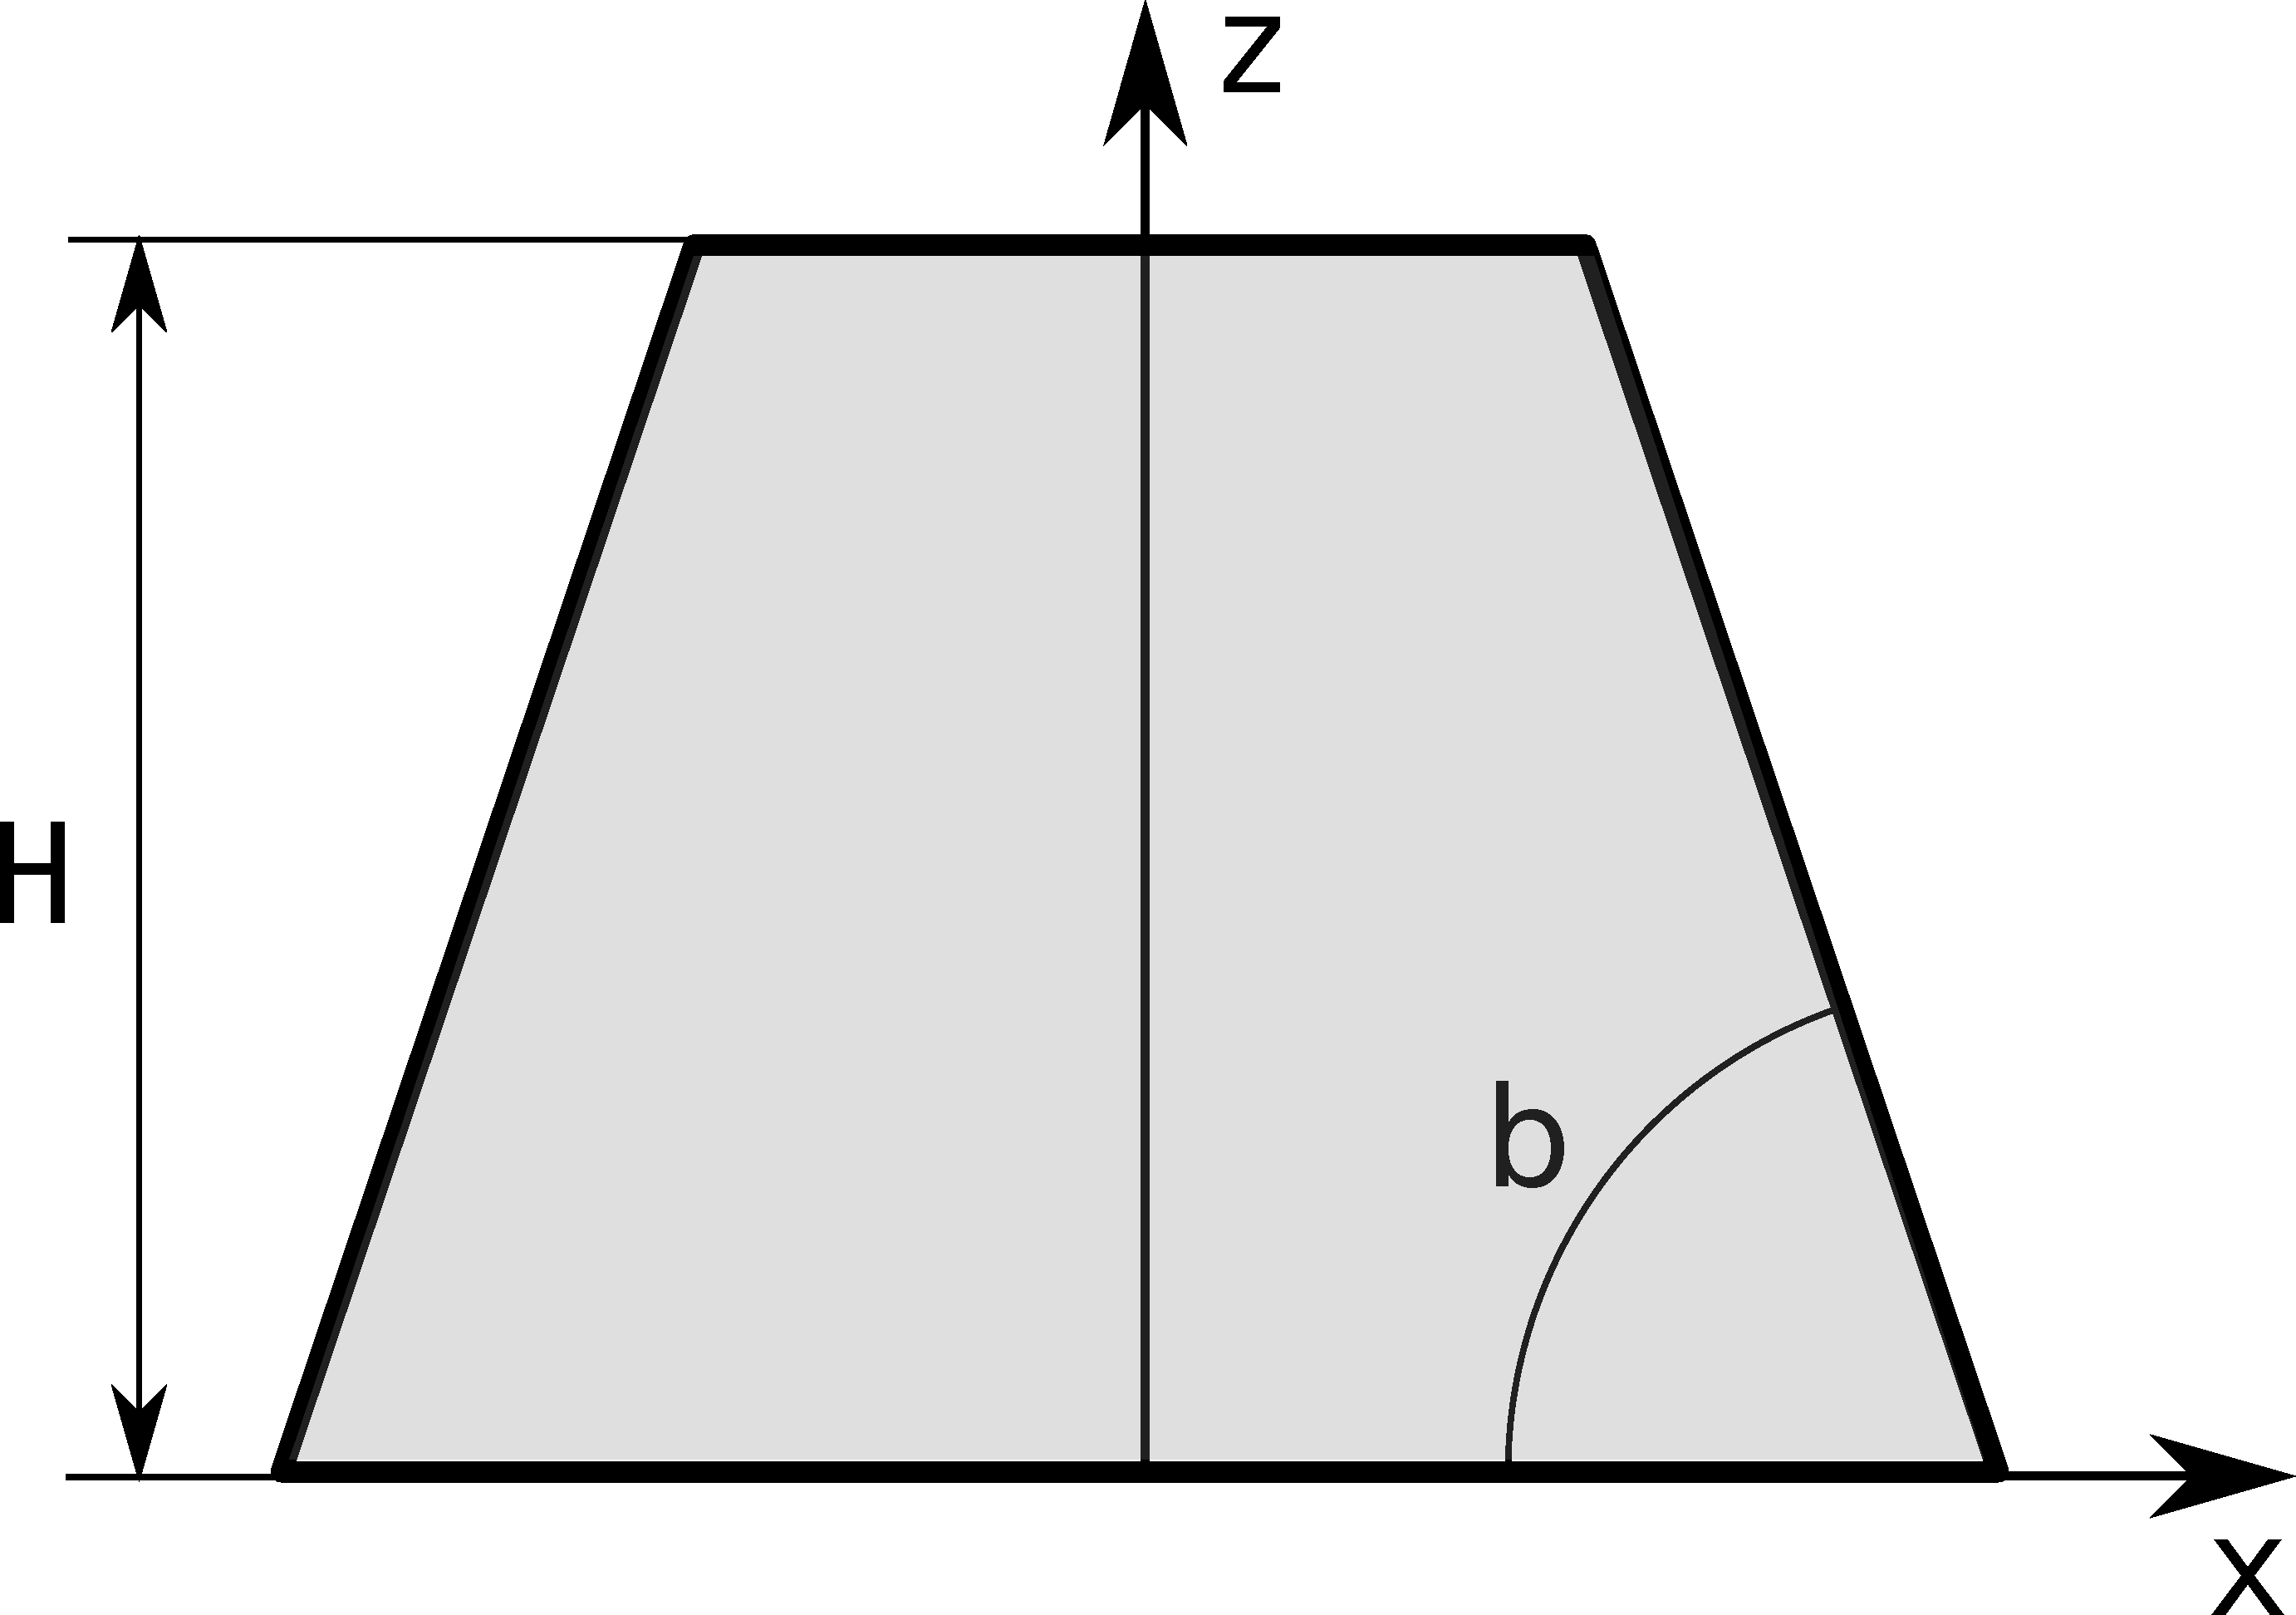
\includegraphics[width=5cm]{fig/cuts/Tetrahedron2dxz.pdf}}
\hfill
\subfigure[Top view]{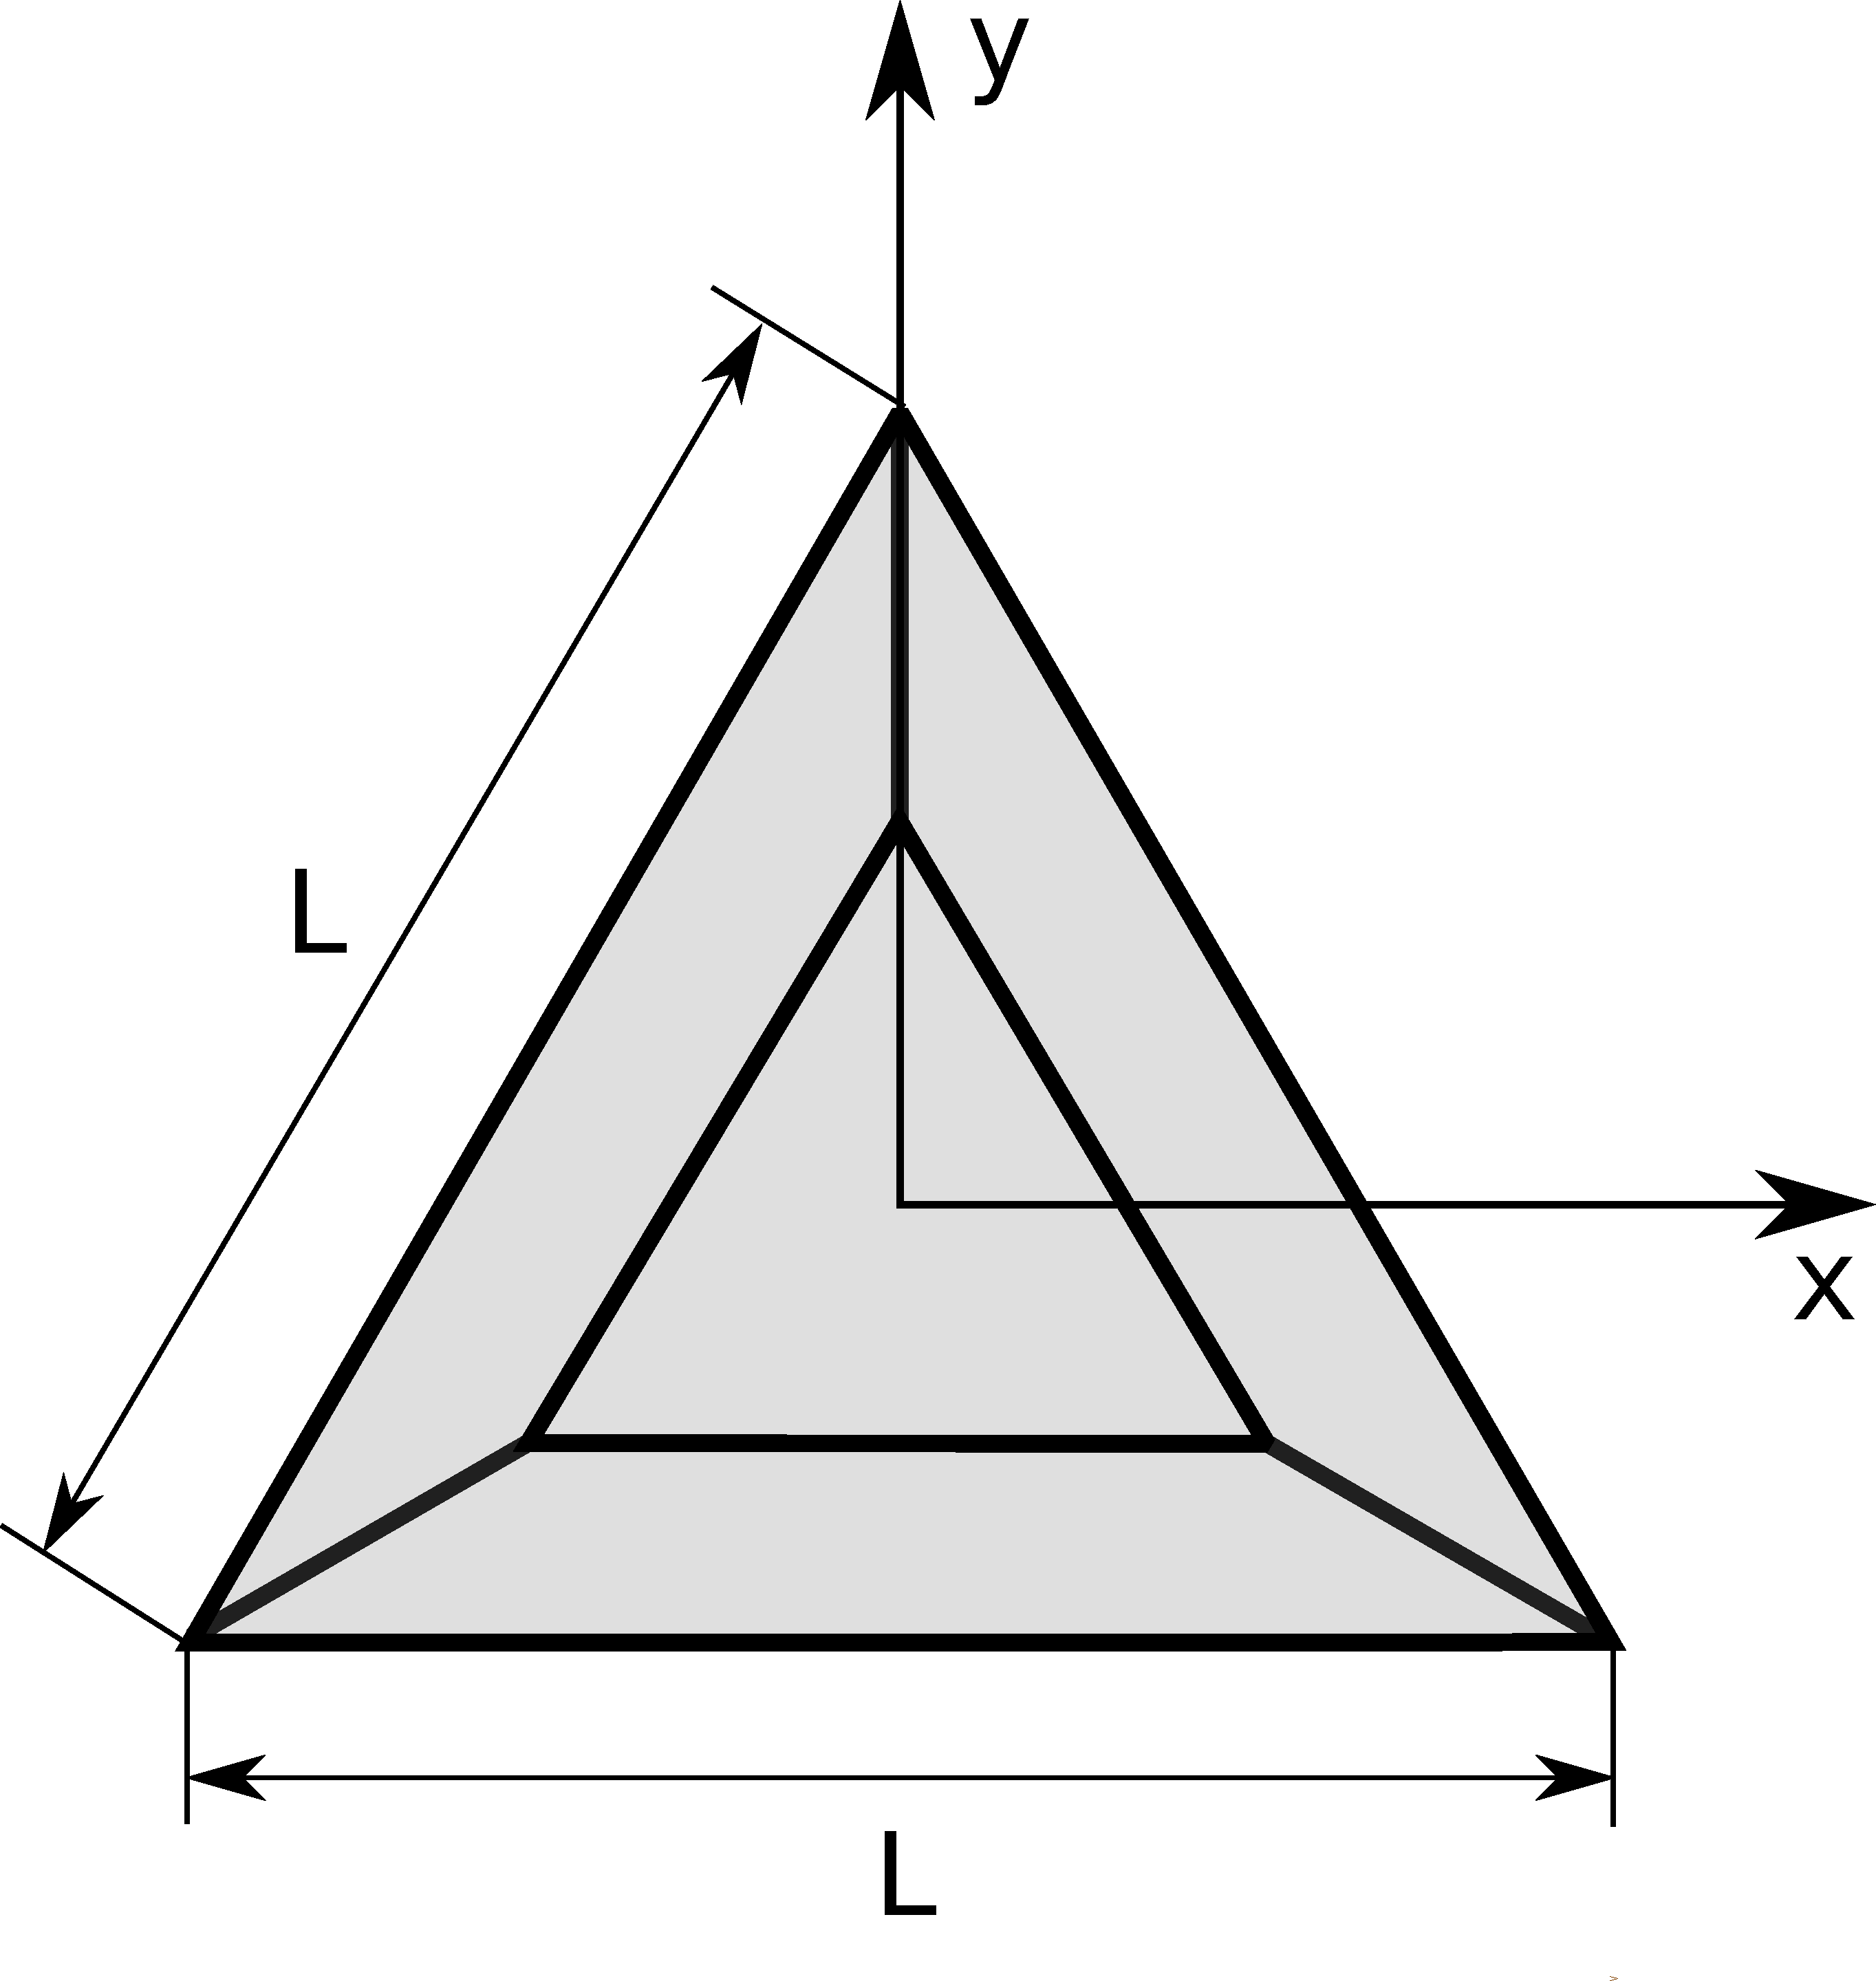
\includegraphics[width=5cm]{fig/cuts/Tetrahedron2dxy.pdf}}
\hfill
\caption{Sketch of a Tetrahedron. The implementation of this shape uses angle
  $\alpha$, which is linked to $\beta$ via $\tan \alpha = 2 \tan 
  \beta$. $\alpha$ is the angle between the base and a side face and $\beta$
  the angle between the base and a side edge.}
\label{fig:tetrahedron}
\end{figure}

\FloatBarrier

\paragraph{Parameters}
\begin{itemize}
\item length of one side of the equilateral triangular base $L$,
\item height $H$,
\item angle $\alpha$ is the angle between the base and the
  side faces.
\end{itemize}

\paragraph{Restrictions on the parameters:} 
$\dfrac{H}{L}< \dfrac{\tan{\alpha}}{2\sqrt{3}}$.

\paragraph{Properties}
\begin{itemize}
\item volume $V= \dfrac{\tan(\alpha) L^3}{24} \left[1- \left(1 -
  \dfrac{2\sqrt{3} H}{L \tan(\alpha)} \right)^3\right]$,
\item particle surface seen from above $S =\dfrac{\sqrt{3}}{4}L^2$.
\end{itemize}

\paragraph{Form factor}

\begin{align*}
&F(\mathbf{q}, L, H, \alpha)=\frac{\sqrt{3}H}{q_x (q_x^2-3q_y^2)}
\exp\left(i\frac{q_z L\tan (\alpha)}{2\sqrt{3}}\right) \times \\
&\Big\{2q_x \exp(iq_3 D)\sinc(q_3 H) - (q_x +\sqrt{3}q_y)
\exp(iq_1 D)\sinc(q_1 H) -(q_x-\sqrt{3}q_y)\exp(-iq_2
D)\sinc(q_2 H) \Big\}, 
\end{align*}
with $\sinc(x)=\sin(x)/x$,
\begin{equation*}
q_1  =\frac{1}{2}\left[\frac{q_x\sqrt{3} -q_y}{\tan \alpha}-q_z \right],
\quad q_2 = \frac{1}{2}\left[\frac{q_x\sqrt{3} +q_y}{\tan \alpha}+q_z
\right], \quad 
q_3 = \frac{q_y}{\tan \alpha} -\frac{q_z}{2}, \quad D = \frac{L \tan \alpha}{\sqrt{3}} -H.
\end{equation*}

\paragraph{Syntax}\strut\\
\Code{FormFactorTetrahedron(length, height, alpha)}

\paragraph{Example}\strut\\
Figure~\ref{fig:FFtetrahEx} shows the normalized intensity
$|F|^2/V^2$, computed with $L=15$~nm, $H=6$~nm and $\alpha =60
^{\circ}$.

\begin{figure}[ht]
\begin{center}
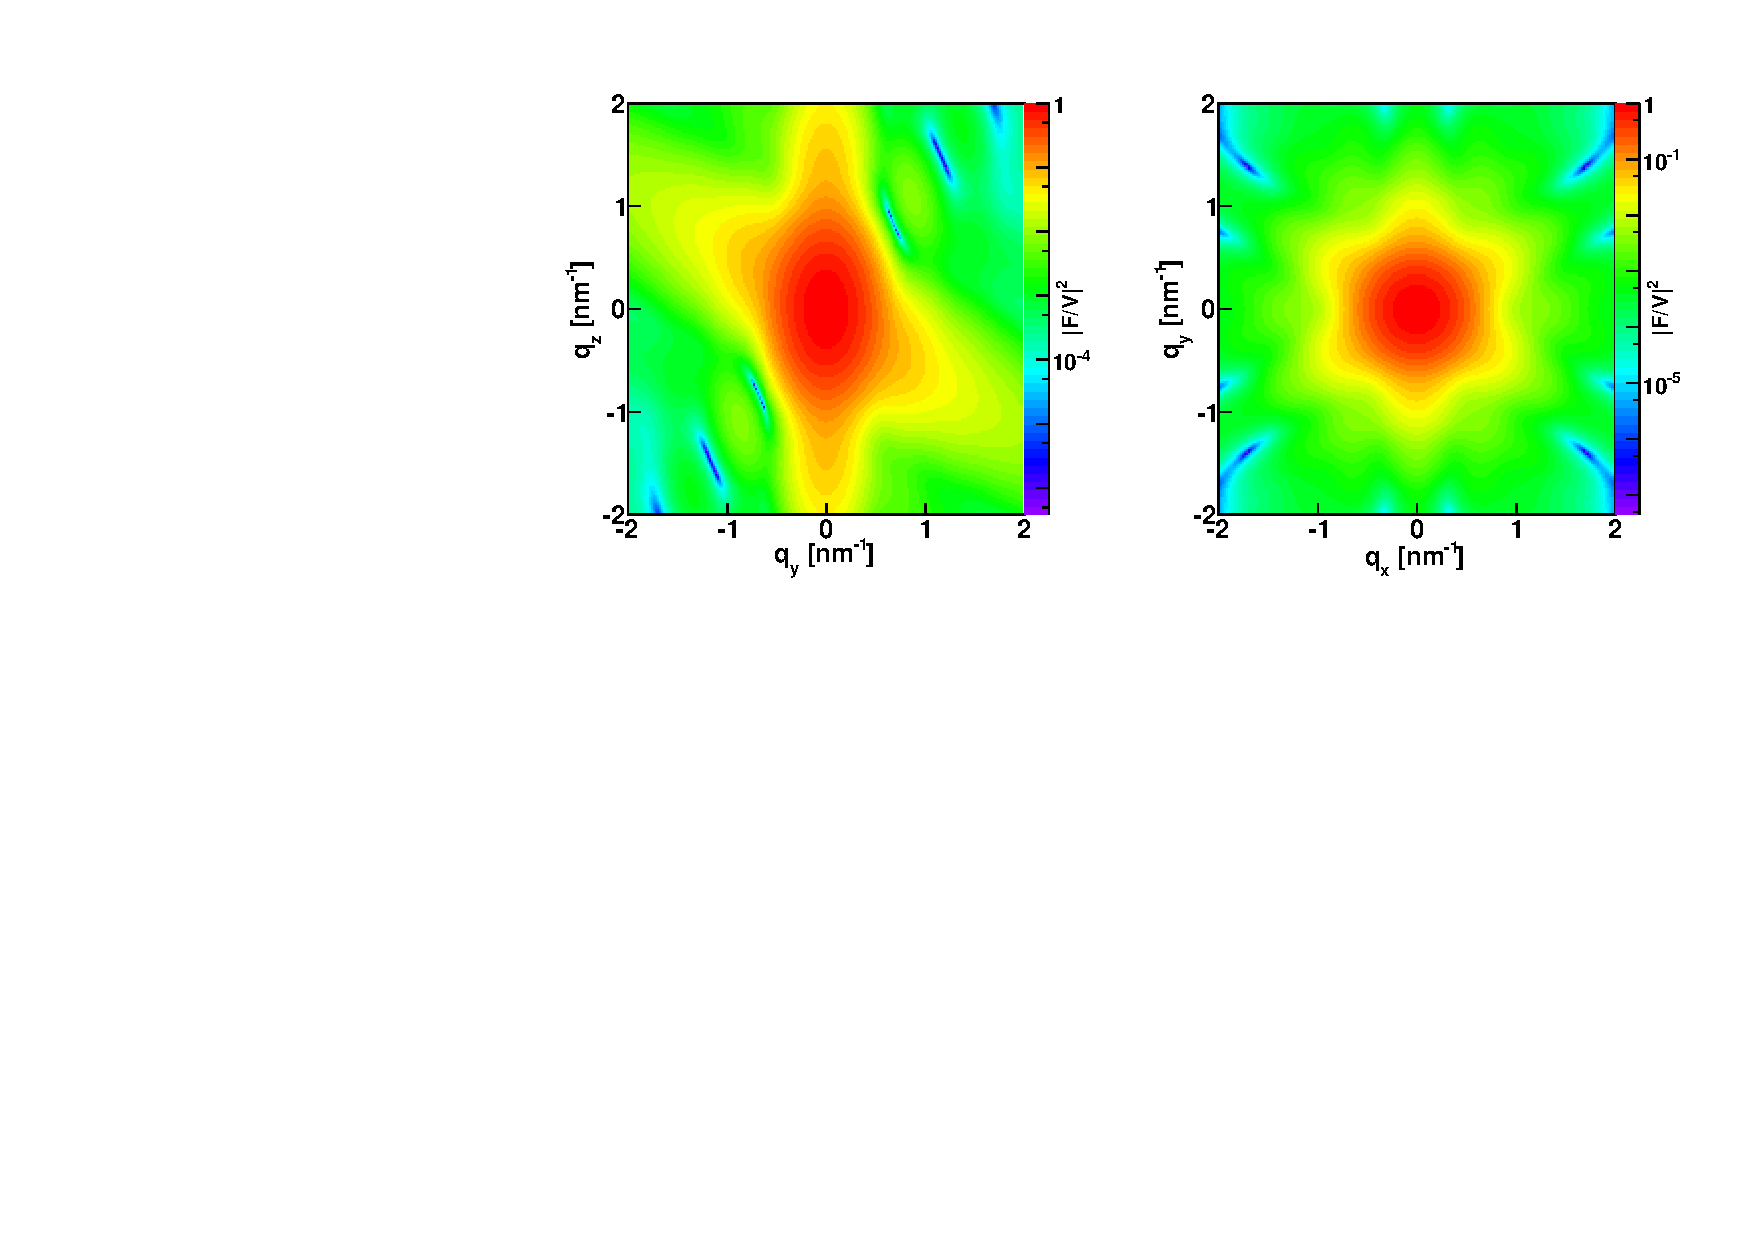
\includegraphics[angle=-90,width=\textwidth]{fig/ff/figfftetrahedron.pdf}
\end{center}
\caption{Normalized intensity for the form factor of a Tetrahedron
  plotted against ($q_y$, $q_z$) and  ($q_x$, $q_y$) and
  computed with \Code{FormFactorTetrahedron(15.*nanometer, 6.*nanometer, 60.*degree)}.}
\label{fig:FFtetrahEx}
\end{figure}

\paragraph{References}\strut\\
??

%-------------------------------------------------------------------------------
\newpage
\subsection{Prism6 (hexagonal)} \label{sec:Prism6}
  \index{Prism (form factor)!hexagonal (Prism6)}
  \index{FormFactorPrism6@\Code{FormFactorPrism6}}
%-------------------------------------------------------------------------------

\paragraph{Real-space geometry}\strut\\
This shape is an hexagonal prism (see fig.~\ref{fig:prism6}).

\begin{figure}[ht]
\hfill
\subfigure[Side view]{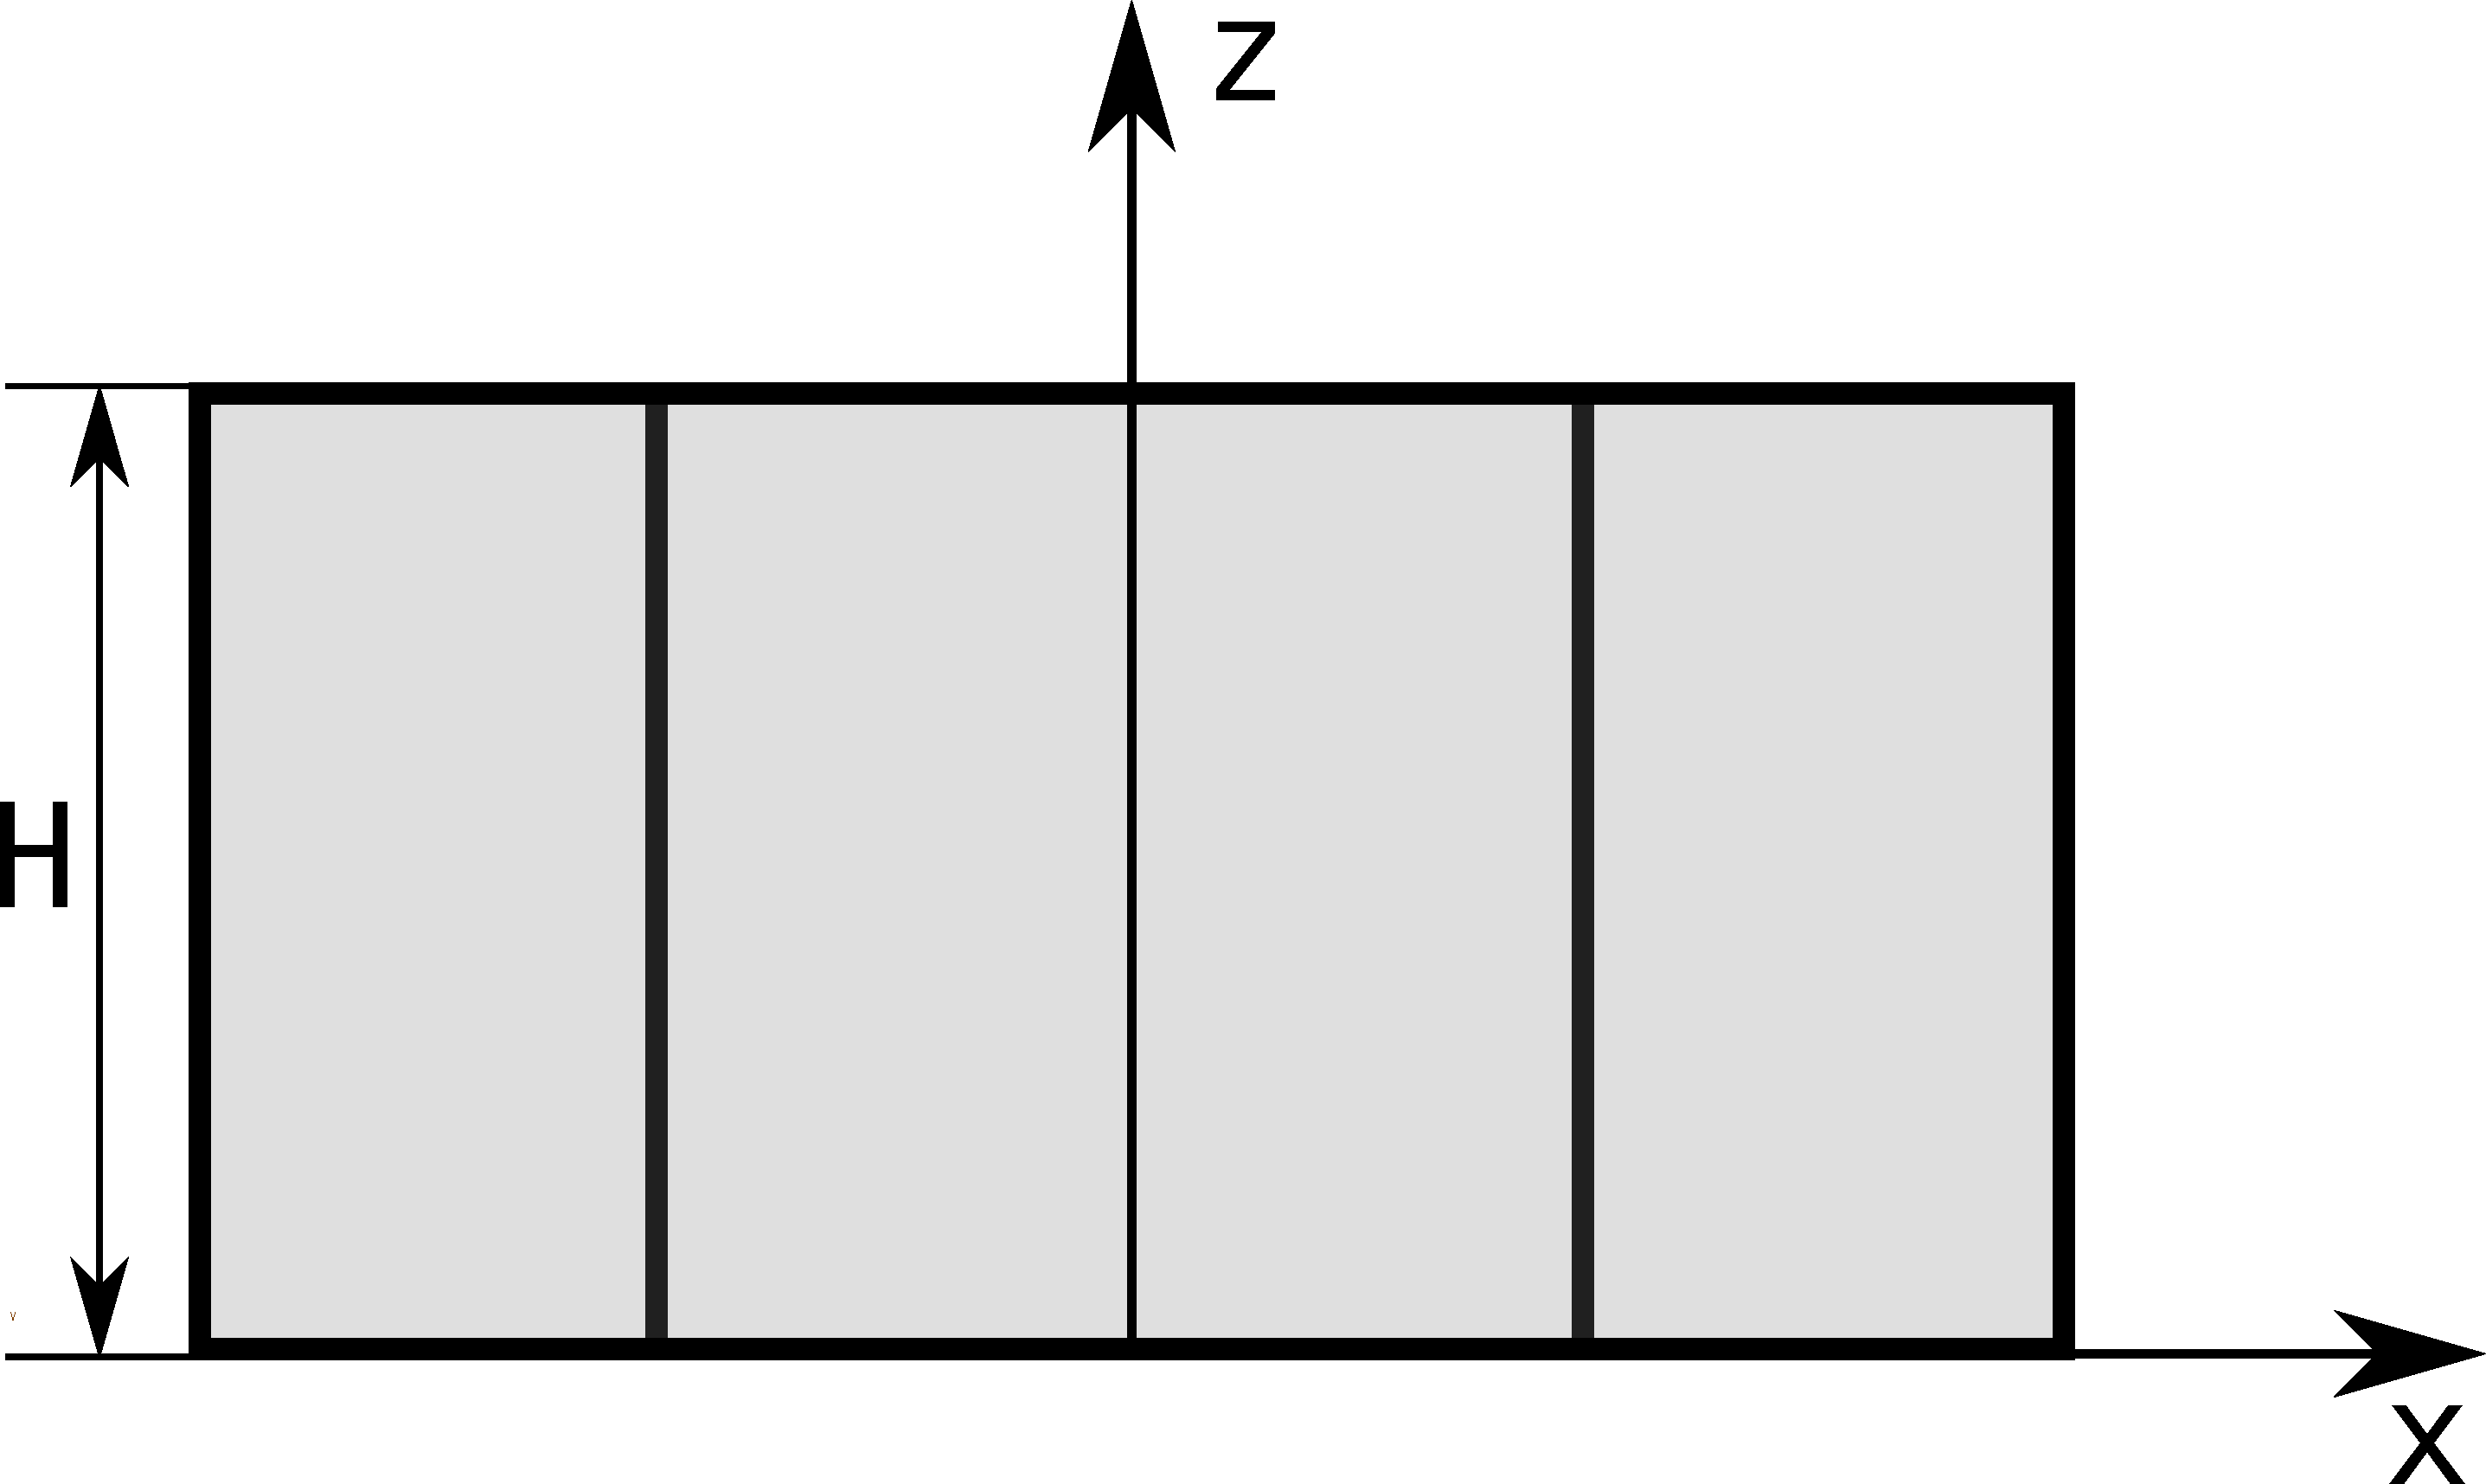
\includegraphics[width=5cm]{fig/cuts/Prism62dxz.pdf}}
\hfill
\subfigure[Top view]{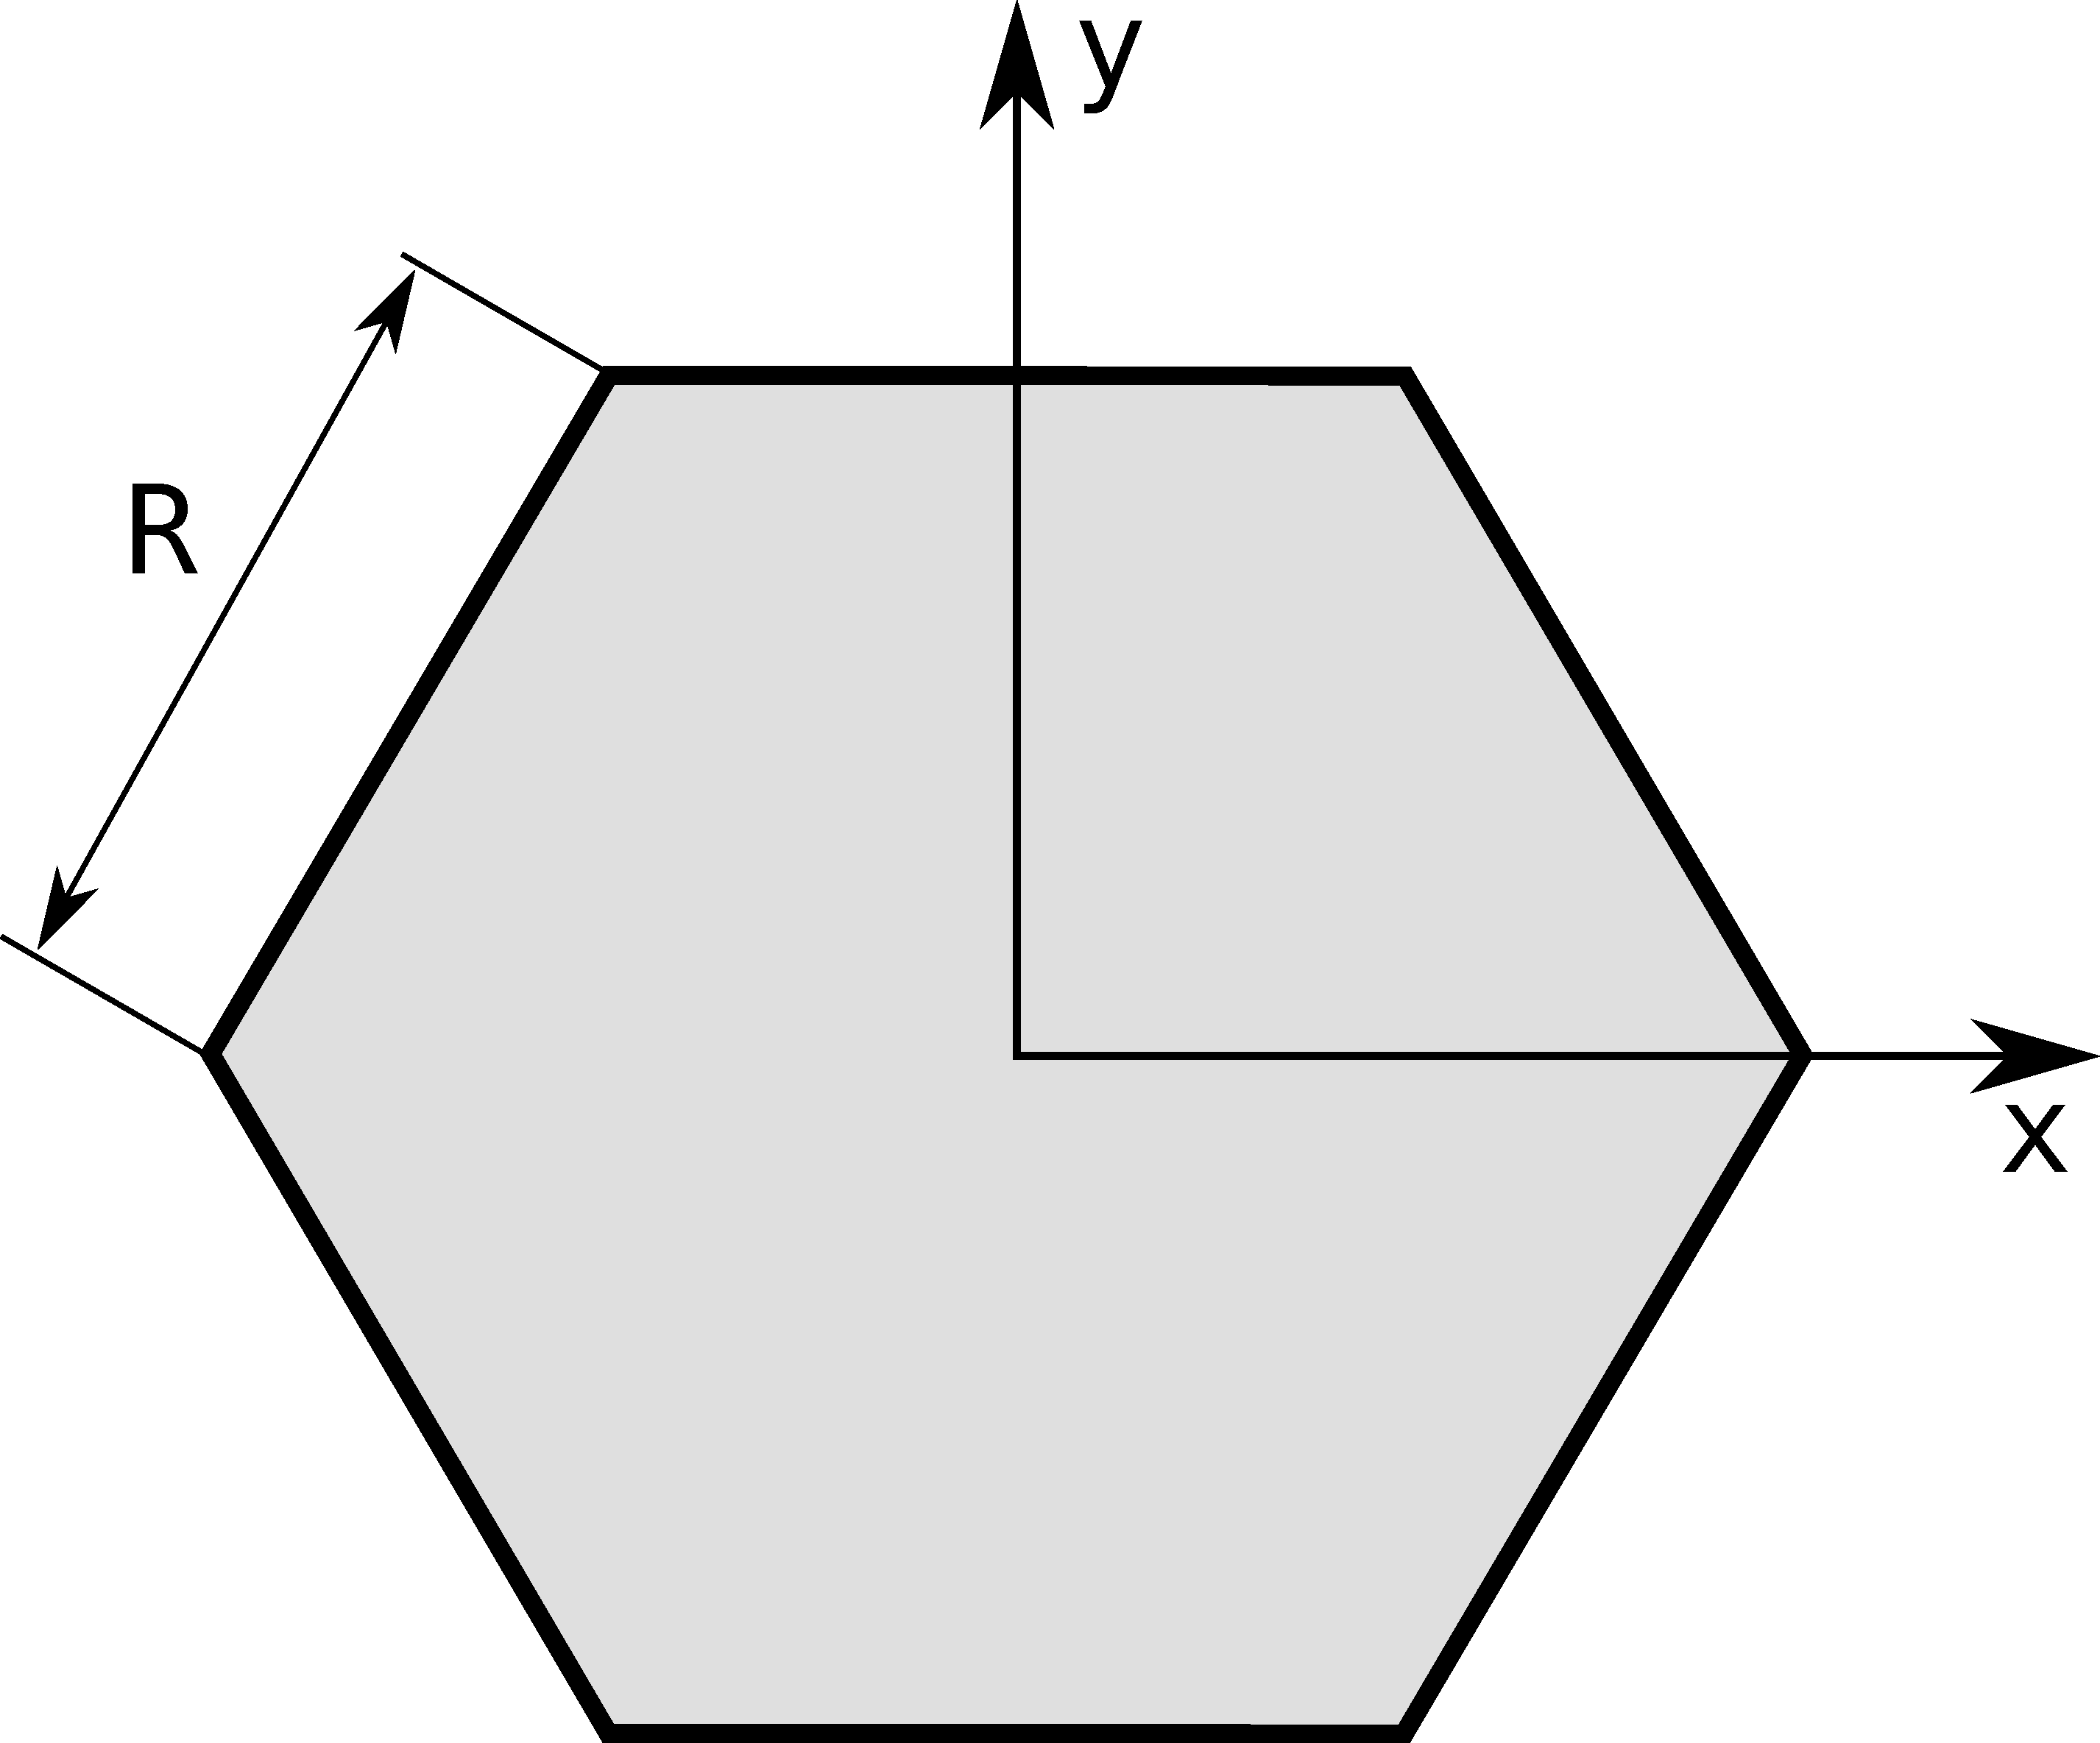
\includegraphics[width=5cm]{fig/cuts/Prism62dxy.pdf}}
\hfill
\caption{Sketch of a Prism6.}
\label{fig:prism6}
\end{figure}

\FloatBarrier

\paragraph{Parameters}
\begin{itemize}
\item radius of the hexagonal base $R$,
\item height $H$.
\end{itemize}

\paragraph{Properties}
\begin{itemize}
\item volume $V = \dfrac{3\sqrt{3}}{2}H R^2$,
\item particle surface seen from above $S =\dfrac{3\sqrt{3}R^2}{2}$.
\end{itemize}

\paragraph{Form factor}
\begin{align*}
F(\mathbf{q}, R, H) &= \frac{4H\sqrt{3}}{3q_y^2 - q_x^2}
\sinc\left(q_z\frac{H}{2}\right) \exp\left(-i q_z\frac{ H}{2}\right)\times\\
&\left\{\frac{3q_y^2R^2}{4} \sinc\left(\frac{q_x
  R}{2}\right)\sinc\left(\frac{\sqrt{3}q_yR }{2}\right)+ \cos(q_x R)-\cos\left(q_y
\frac{\sqrt{3}R}{2}\right) \cos\left(\frac{q_x R}{2}\right)\right\},
\end{align*}
with $\sinc(x)=\sin(x)/x$.

\paragraph{Syntax}\strut\\
\Code{FormFactorPrism6(radius, height)} 

\newpage

\paragraph{Example}\strut\\
Figure~\ref{fig:FFprism6Ex} shows the normalized intensity
$|F|^2/V^2$, computed with $R=5$~nm and \mbox{$H=11$~nm.}

\begin{figure}[ht]
\begin{center}
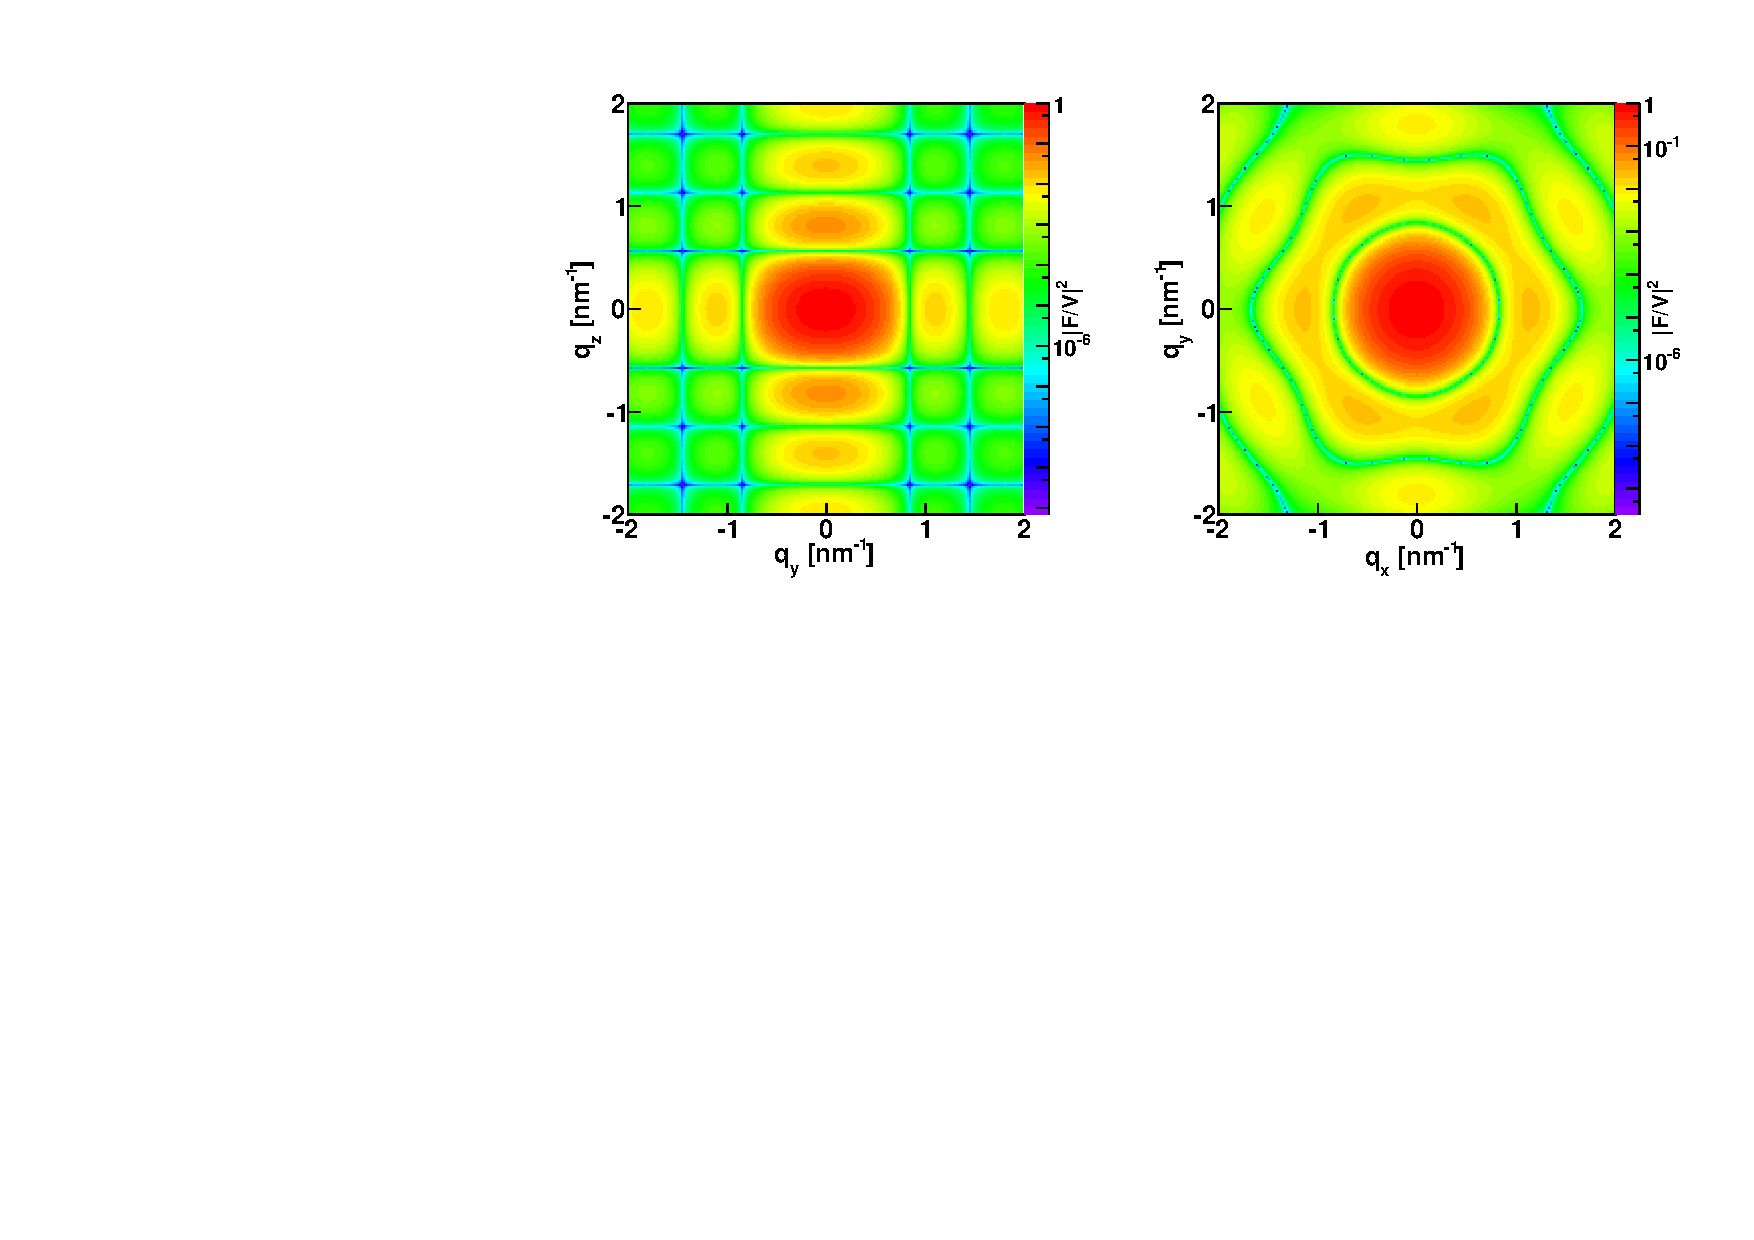
\includegraphics[angle=-90,width=\textwidth]{fig/ff/figffprism6.pdf}
\end{center}
\caption{Normalized intensity for the form factor of a Prism6 plotted against ($q_y$, $q_z$) and ($q_x$, $q_y$) and computed with \Code{FormFactorPrism6(5.*nanometer, 11.*nanometer)}.}
\label{fig:FFprism6Ex}
\end{figure}

\paragraph{References}\strut\\
Agrees with \lq\lq Prism6\rq\rq\ form factor of \IsGISAXS~\cite{Laz02},
except for different parametrization,
and for a factor $H$ missing in the \Code{IsGISAXS} manual. 

%-------------------------------------------------------------------------------
\newpage
\subsection{Cone6 (hexagonal)} \label{sec:Cone6}
  \index{Cone (form factor)!hexagonal (Cone6)}
  \index{Pyramid (form factor)!hexagonal (Cone6)}
  \index{Truncated pyramid (form factor)!hexagonal (Cone6)}
  \index{FormFactorCone6@\Code{FormFactorCone6}}
%-------------------------------------------------------------------------------

\paragraph{Real-space geometry}\strut\\
It is a truncated hexagonal pyramid (see fig.~\ref{fig:cone6}). 

\begin{figure}[ht]
\hfill
\subfigure[Side view]{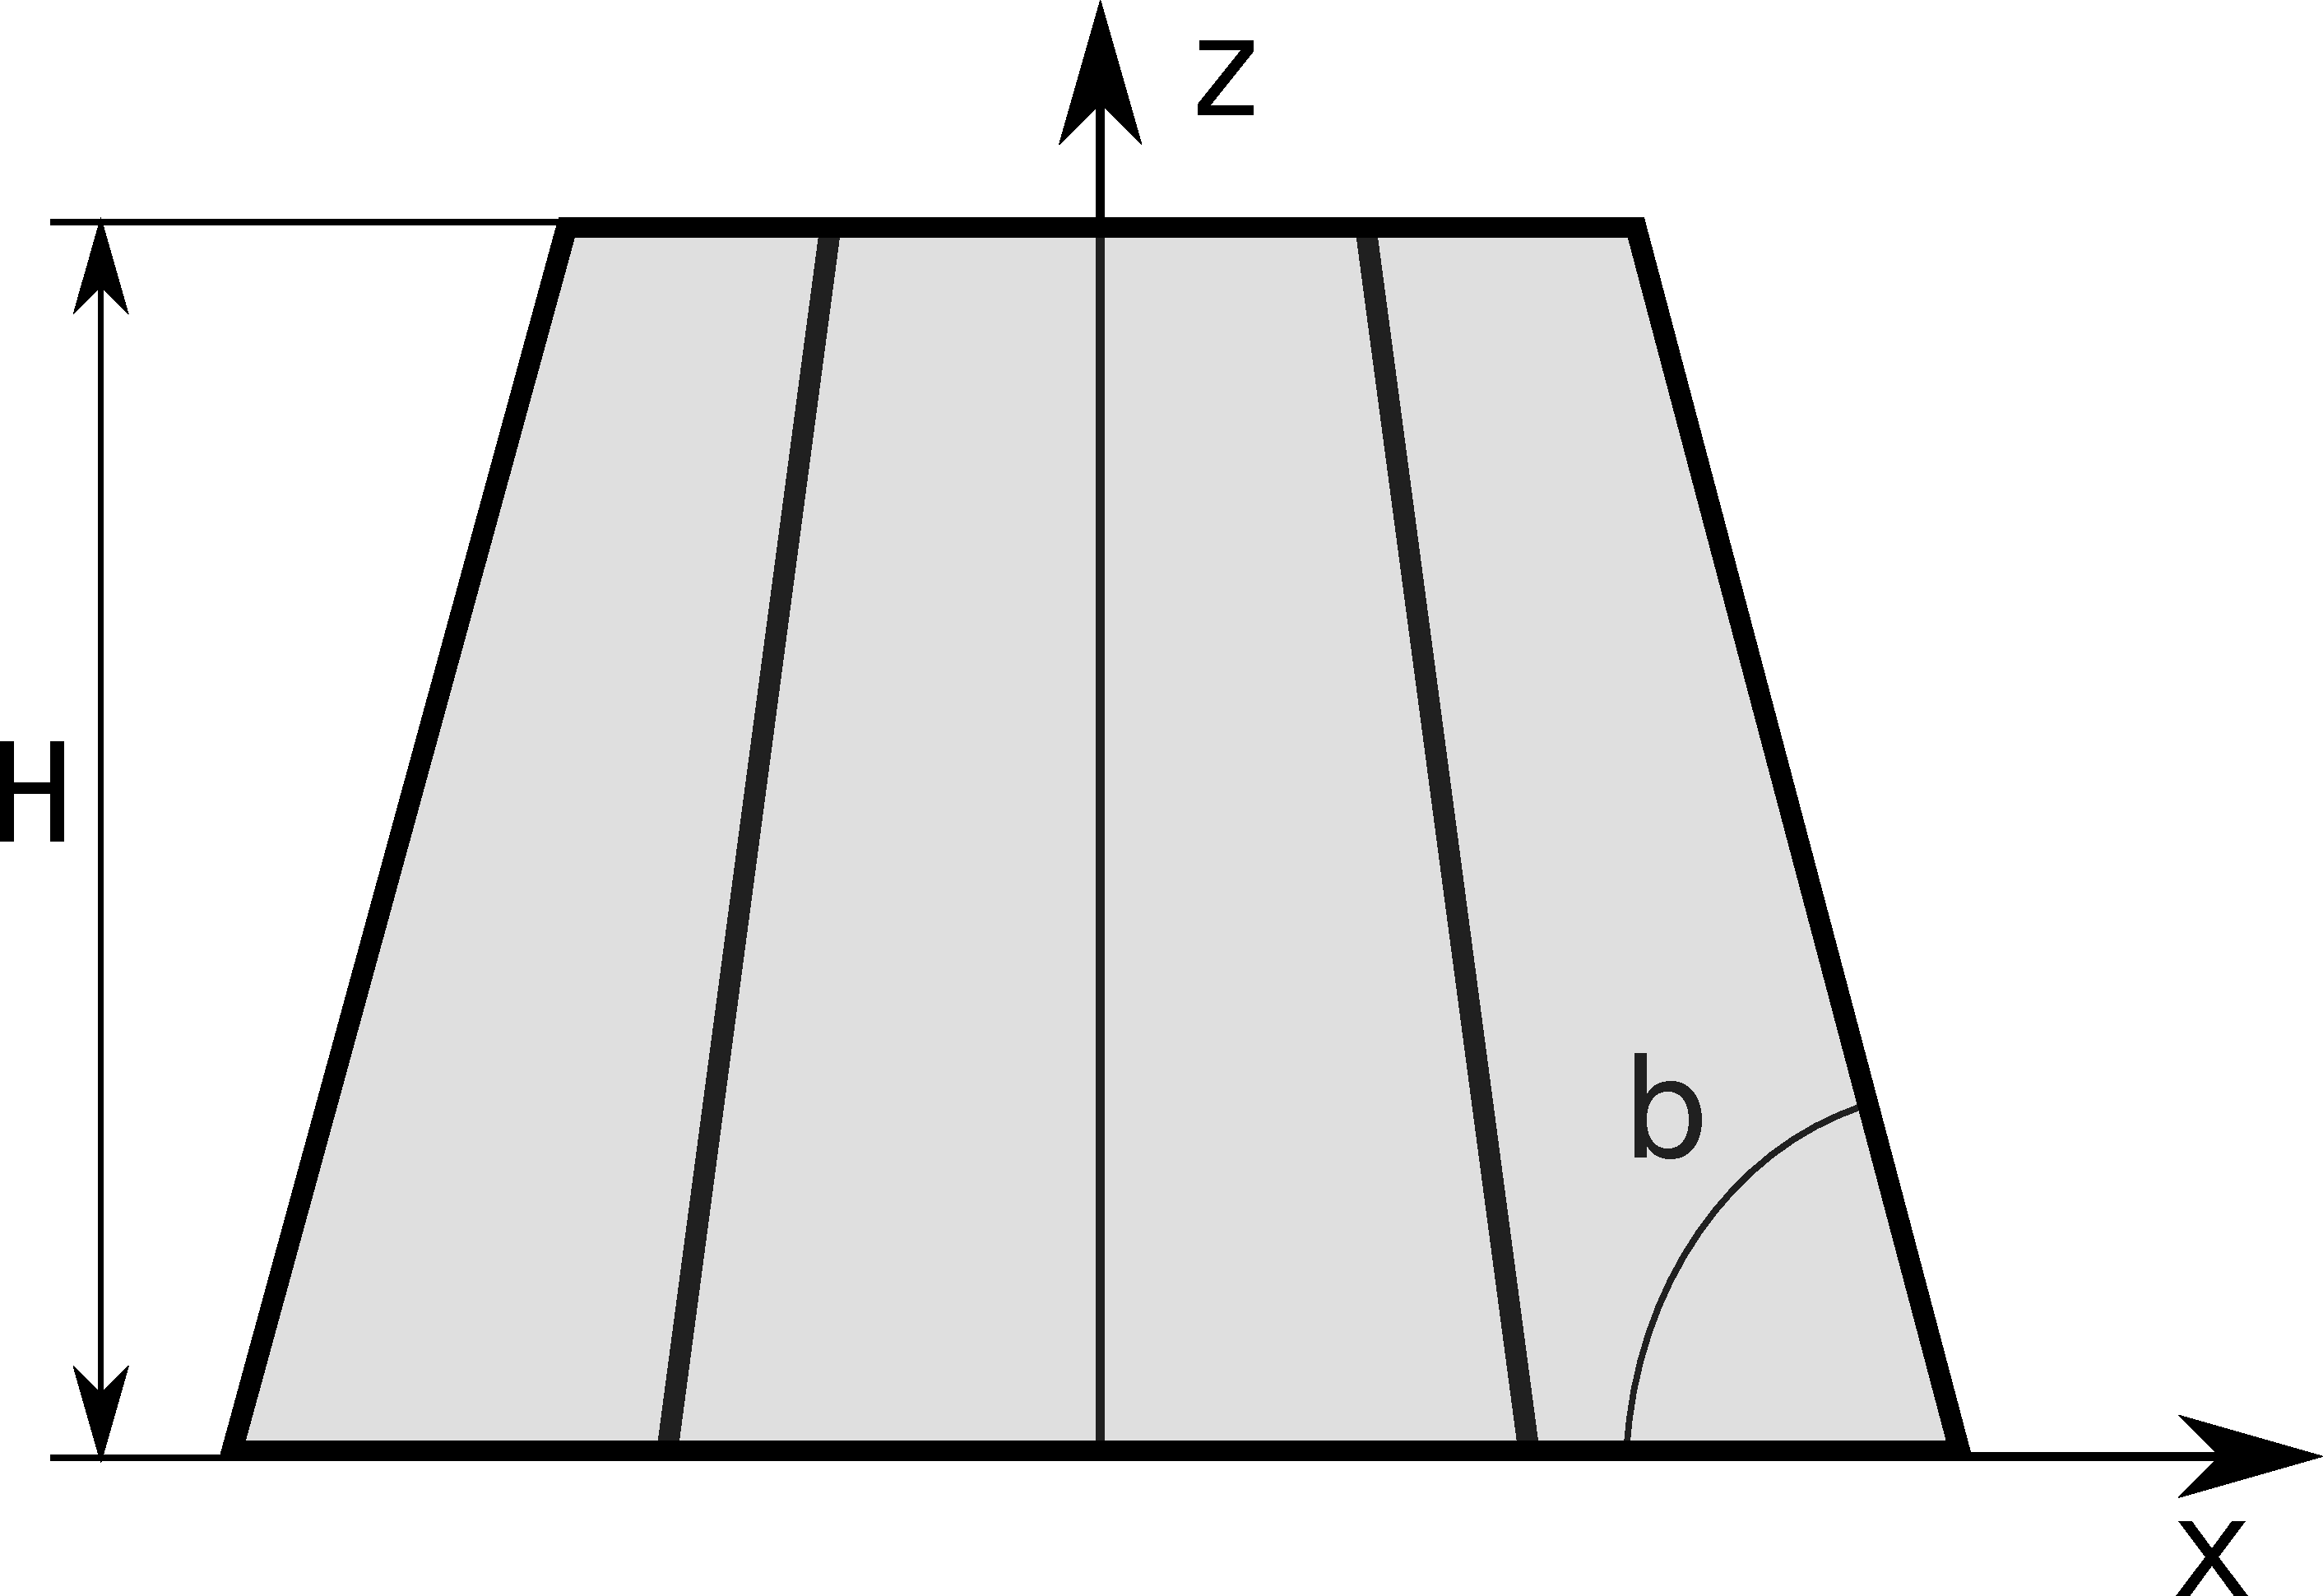
\includegraphics[width=5cm]{fig/cuts/Cone62dxz.pdf}}
\hfill
\subfigure[Top view]{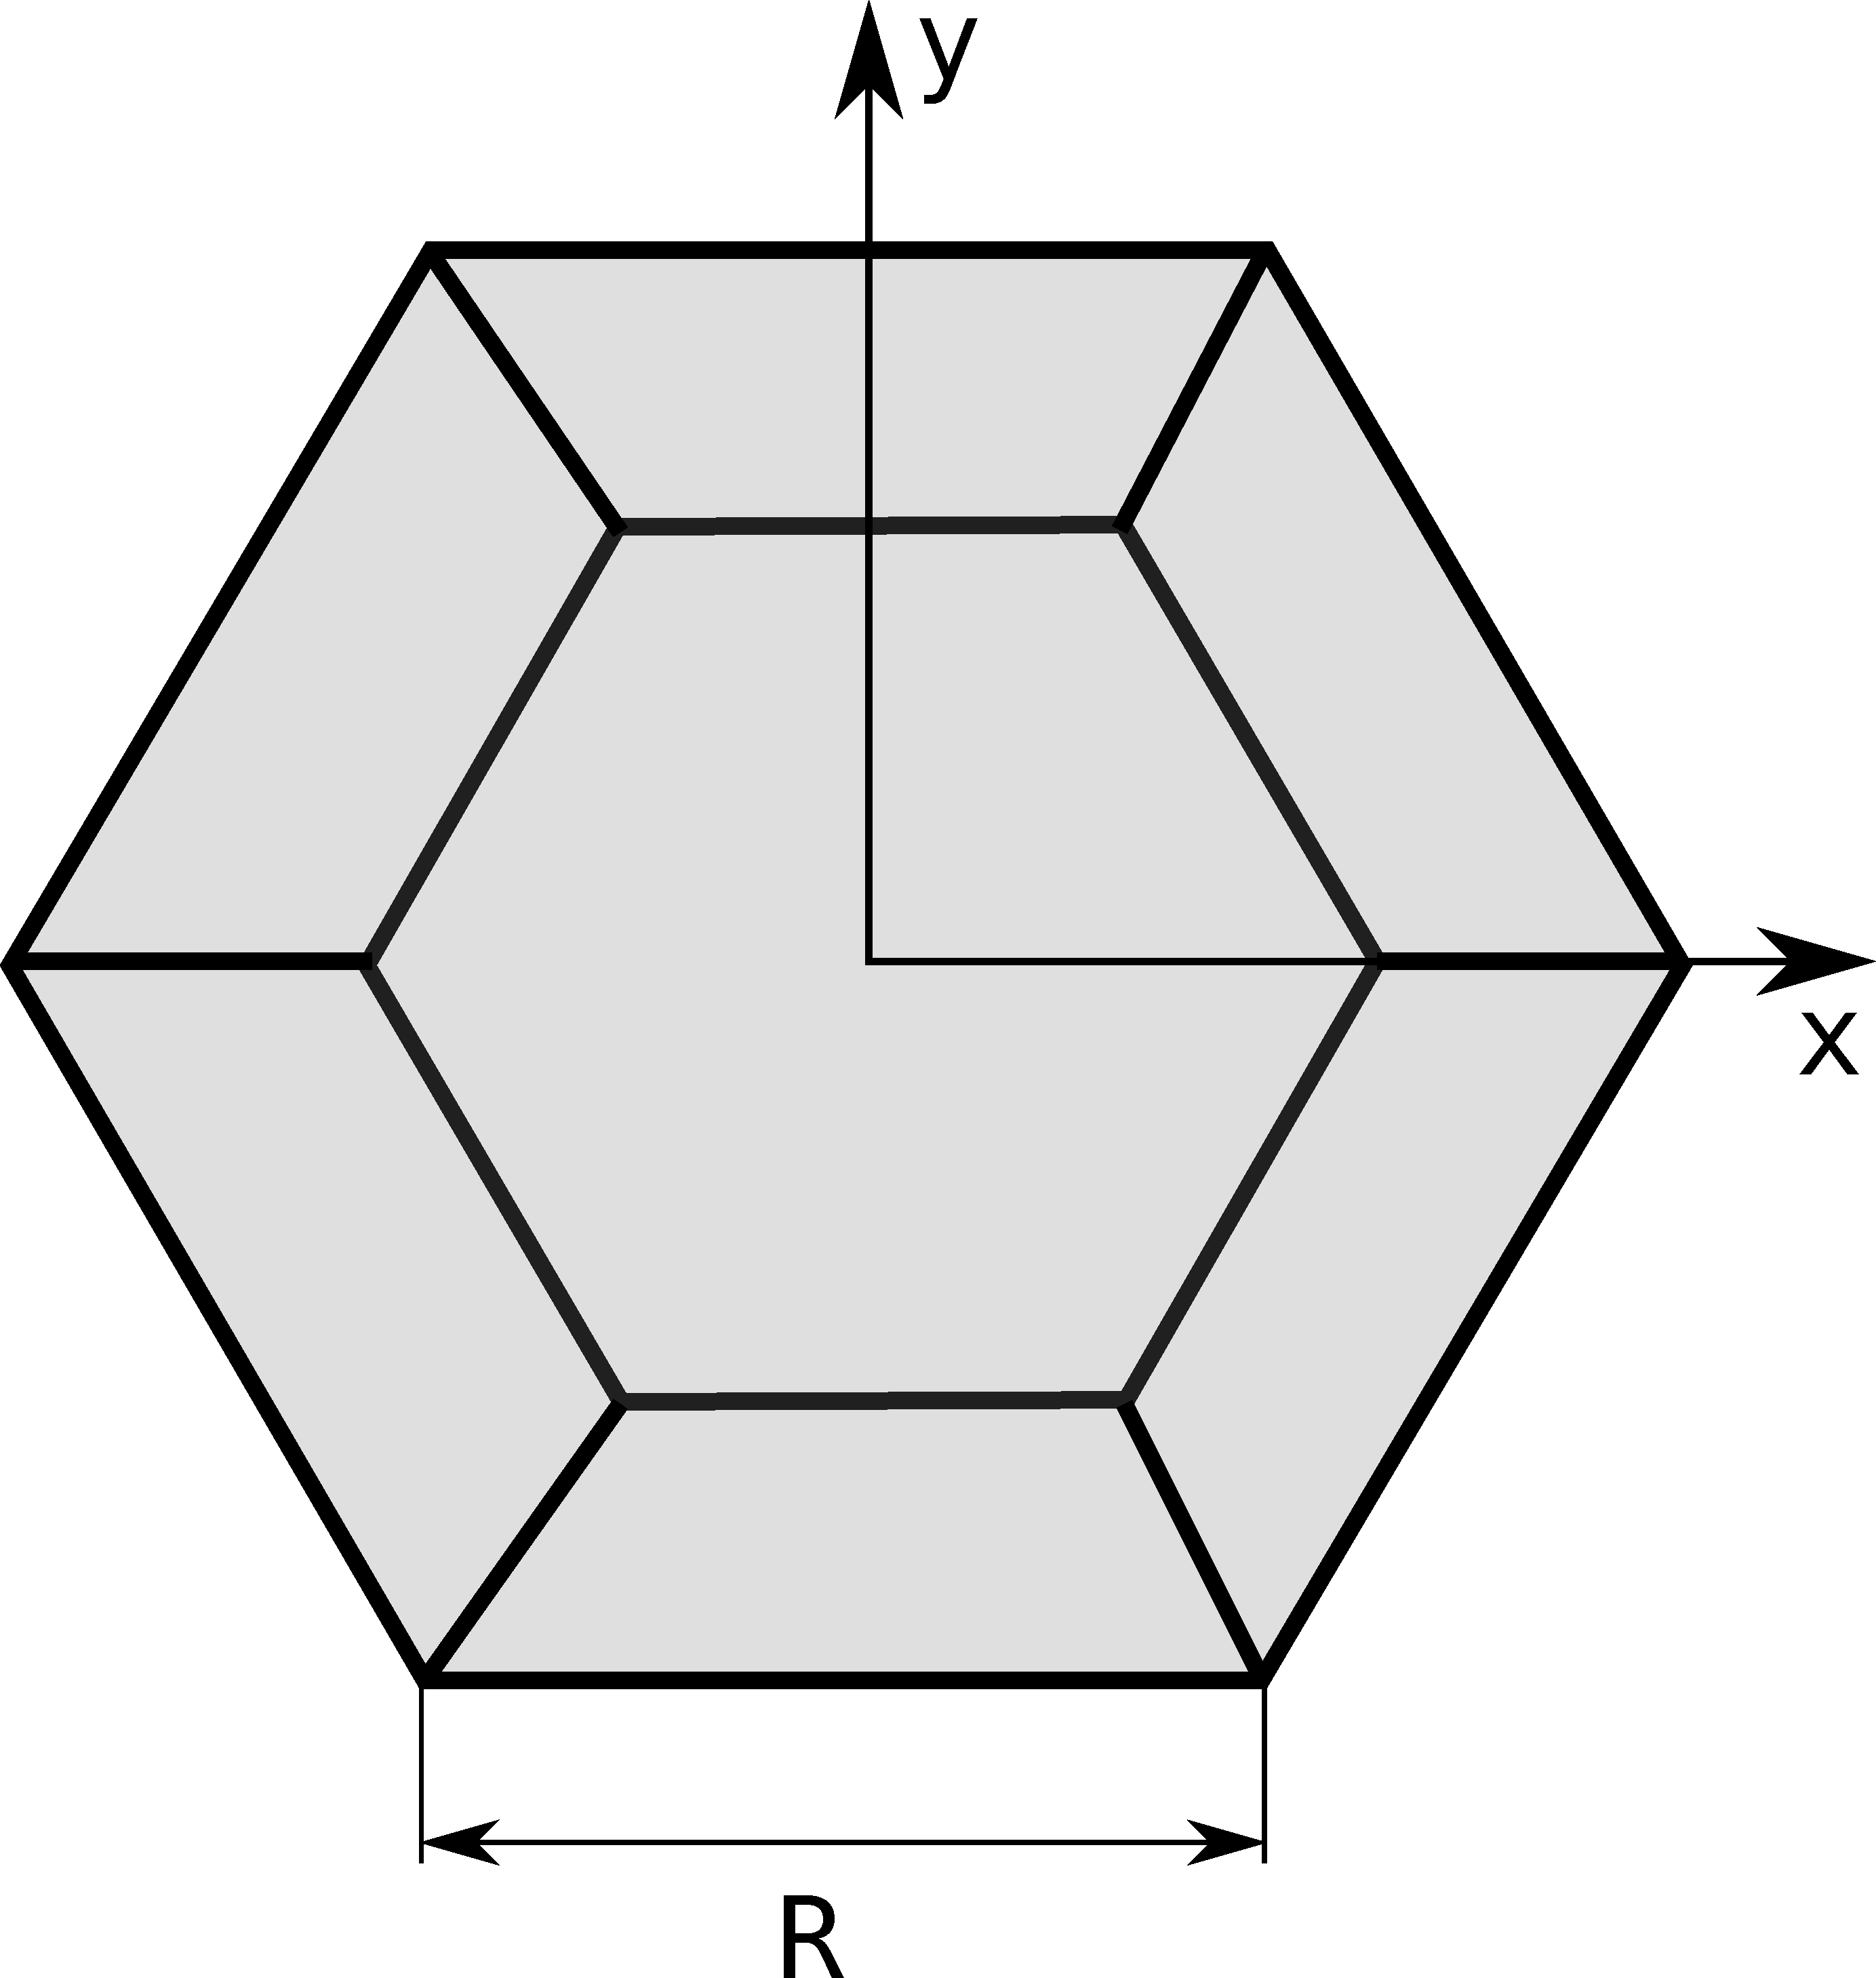
\includegraphics[width=5cm]{fig/cuts/Cone62dxy.pdf}}
\hfill
\caption{Sketch of a Cone6.  The implementation of this shape uses angle
  $\alpha$, which is linked to $\beta$ via $\tan \alpha = \dfrac{2}{\sqrt{3}} \tan 
  \beta$. $\alpha$ is measured along one of the base lines and $\beta$
  at one of the base vertices.}
\label{fig:cone6}
\end{figure}

\FloatBarrier

\paragraph{Parameters}
\begin{itemize}
\item radius of the regular hexagonal base $R$,
\item height $H$,
\item angle $\alpha$ is considered between one of the side faces and
  the middle of a base length. 
\end{itemize}

\paragraph{Restrictions on the parameters:} 
$\dfrac{2H}{\sqrt{3}R}< \tan{\alpha}$.

\paragraph{Properties}
\begin{itemize}
\item volume $V = \dfrac{3}{4} \tan(\alpha) R^3 \left[
            1 - \left(1- \dfrac{2H}{ \tan(\alpha) R\sqrt{3}}\right)^3
            \right]$,
\item  particle surface seen from above $S =\dfrac{3\sqrt{3}R^2}{2}$.
\end{itemize}

\paragraph{Form factor}\strut\\
The calculation can be derived from ``Prism6'' (Sect.~\ref{sec:Prism6}) by
considering a side length varying with the vertical position:

\begin{align*}
F(\mathbf{q}, R, H, \alpha) = \frac{4\sqrt{3}}{3q_y ^2 - q_x^2}\int_0 ^H &\exp(iq_z z)
\Big[\frac{3}{4}R_z^2q_y^2 \sinc\left(\frac{q_xR_z}{2}\right)\sinc\left(\frac{\sqrt{3}q_y
R_z}{2}\right)\\
&+\cos(q_xR_z)-\cos\left(\frac{\sqrt{3}q_y R_z}{2}\right)\cos\left(\frac{q_xR_z}{2}\right) \Big]dz
\end{align*}
with $R_z=R-\dfrac{2z}{\sqrt{3}\tan(\alpha)}$ and $\sinc(x)=\sin(x)/x$.

\paragraph{Syntax}\strut\\
\Code{FormFactorCone6(radius,height, alpha)} 

\paragraph{Example}\strut\\
Figure~\ref{fig:FFCone6Ex} shows the normalized intensity
$|F|^2/V^2$, computed with $R=10$~nm, $H=13$~nm, and
$\alpha=60^{\circ}$.

\begin{figure}[ht]
\begin{center}
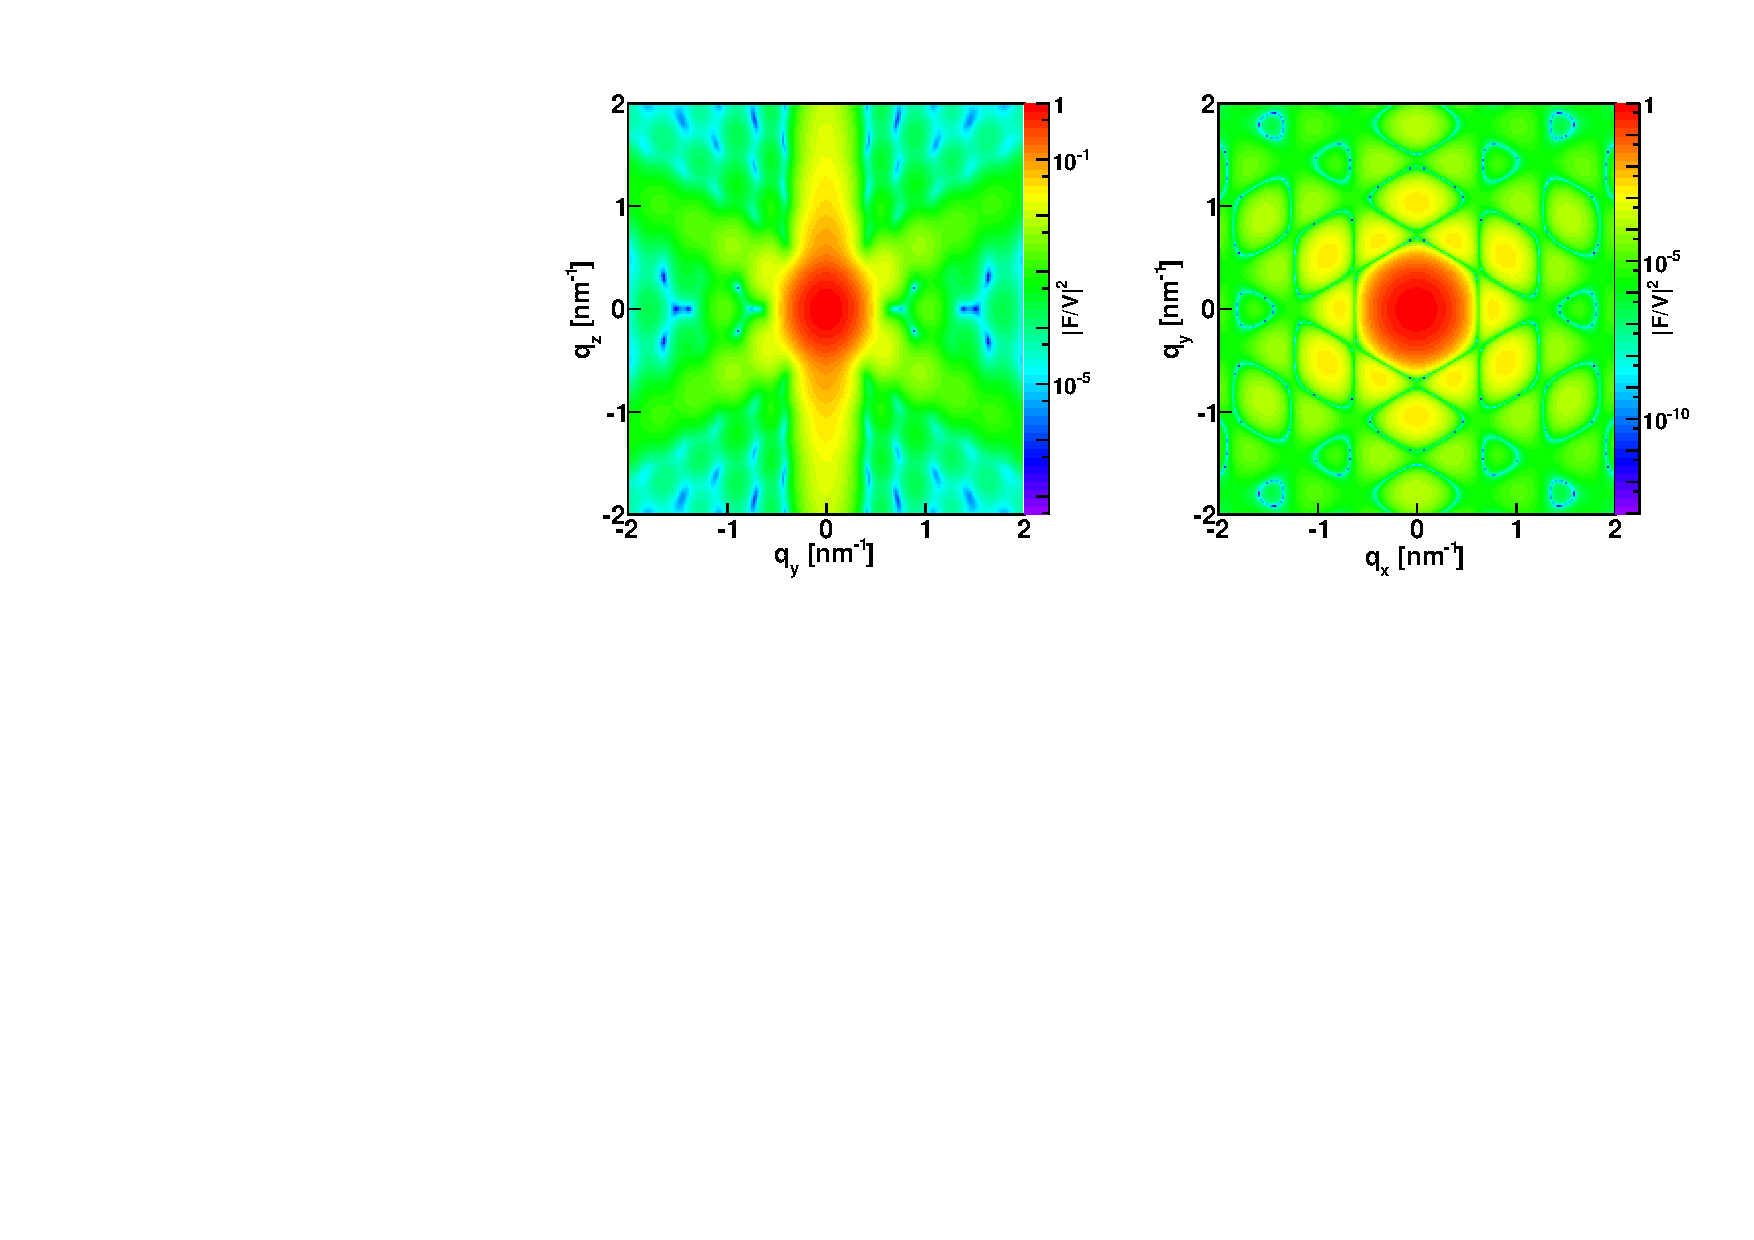
\includegraphics[angle=-90,width=\textwidth]{fig/ff/figffcone6.pdf}
\end{center}
\caption{Normalized intensity for the form factor of a Cone6 plotted against ($q_y$, $q_z$) and ($q_x$, $q_y$) and computed with \Code{FormFactorCone6(10.*nanometer, 13.*nanometer, 60.*degree)}.}
\label{fig:FFCone6Ex}
\end{figure}

\paragraph{References}\strut\\
Agrees with \lq\lq Cone6\rq\rq\ form factor of \IsGISAXS~\cite{Laz02} ???

%-------------------------------------------------------------------------------
\newpage
\subsection{Pyramid (square-based)}\label{sec:Pyramid}
  \index{Pyramid (form factor)!square}
  \index{Truncated pyramid (form factor)!square}
  \index{FormFactorPyramid@\Code{FormFactorPyramid}}
%-------------------------------------------------------------------------------

\paragraph{Real-space geometry}\strut\\
A truncated pyramid with a square base as shown in fig.~\ref{fig:pyramid}.

\begin{figure}[ht]
\hfill
\subfigure[Side view]{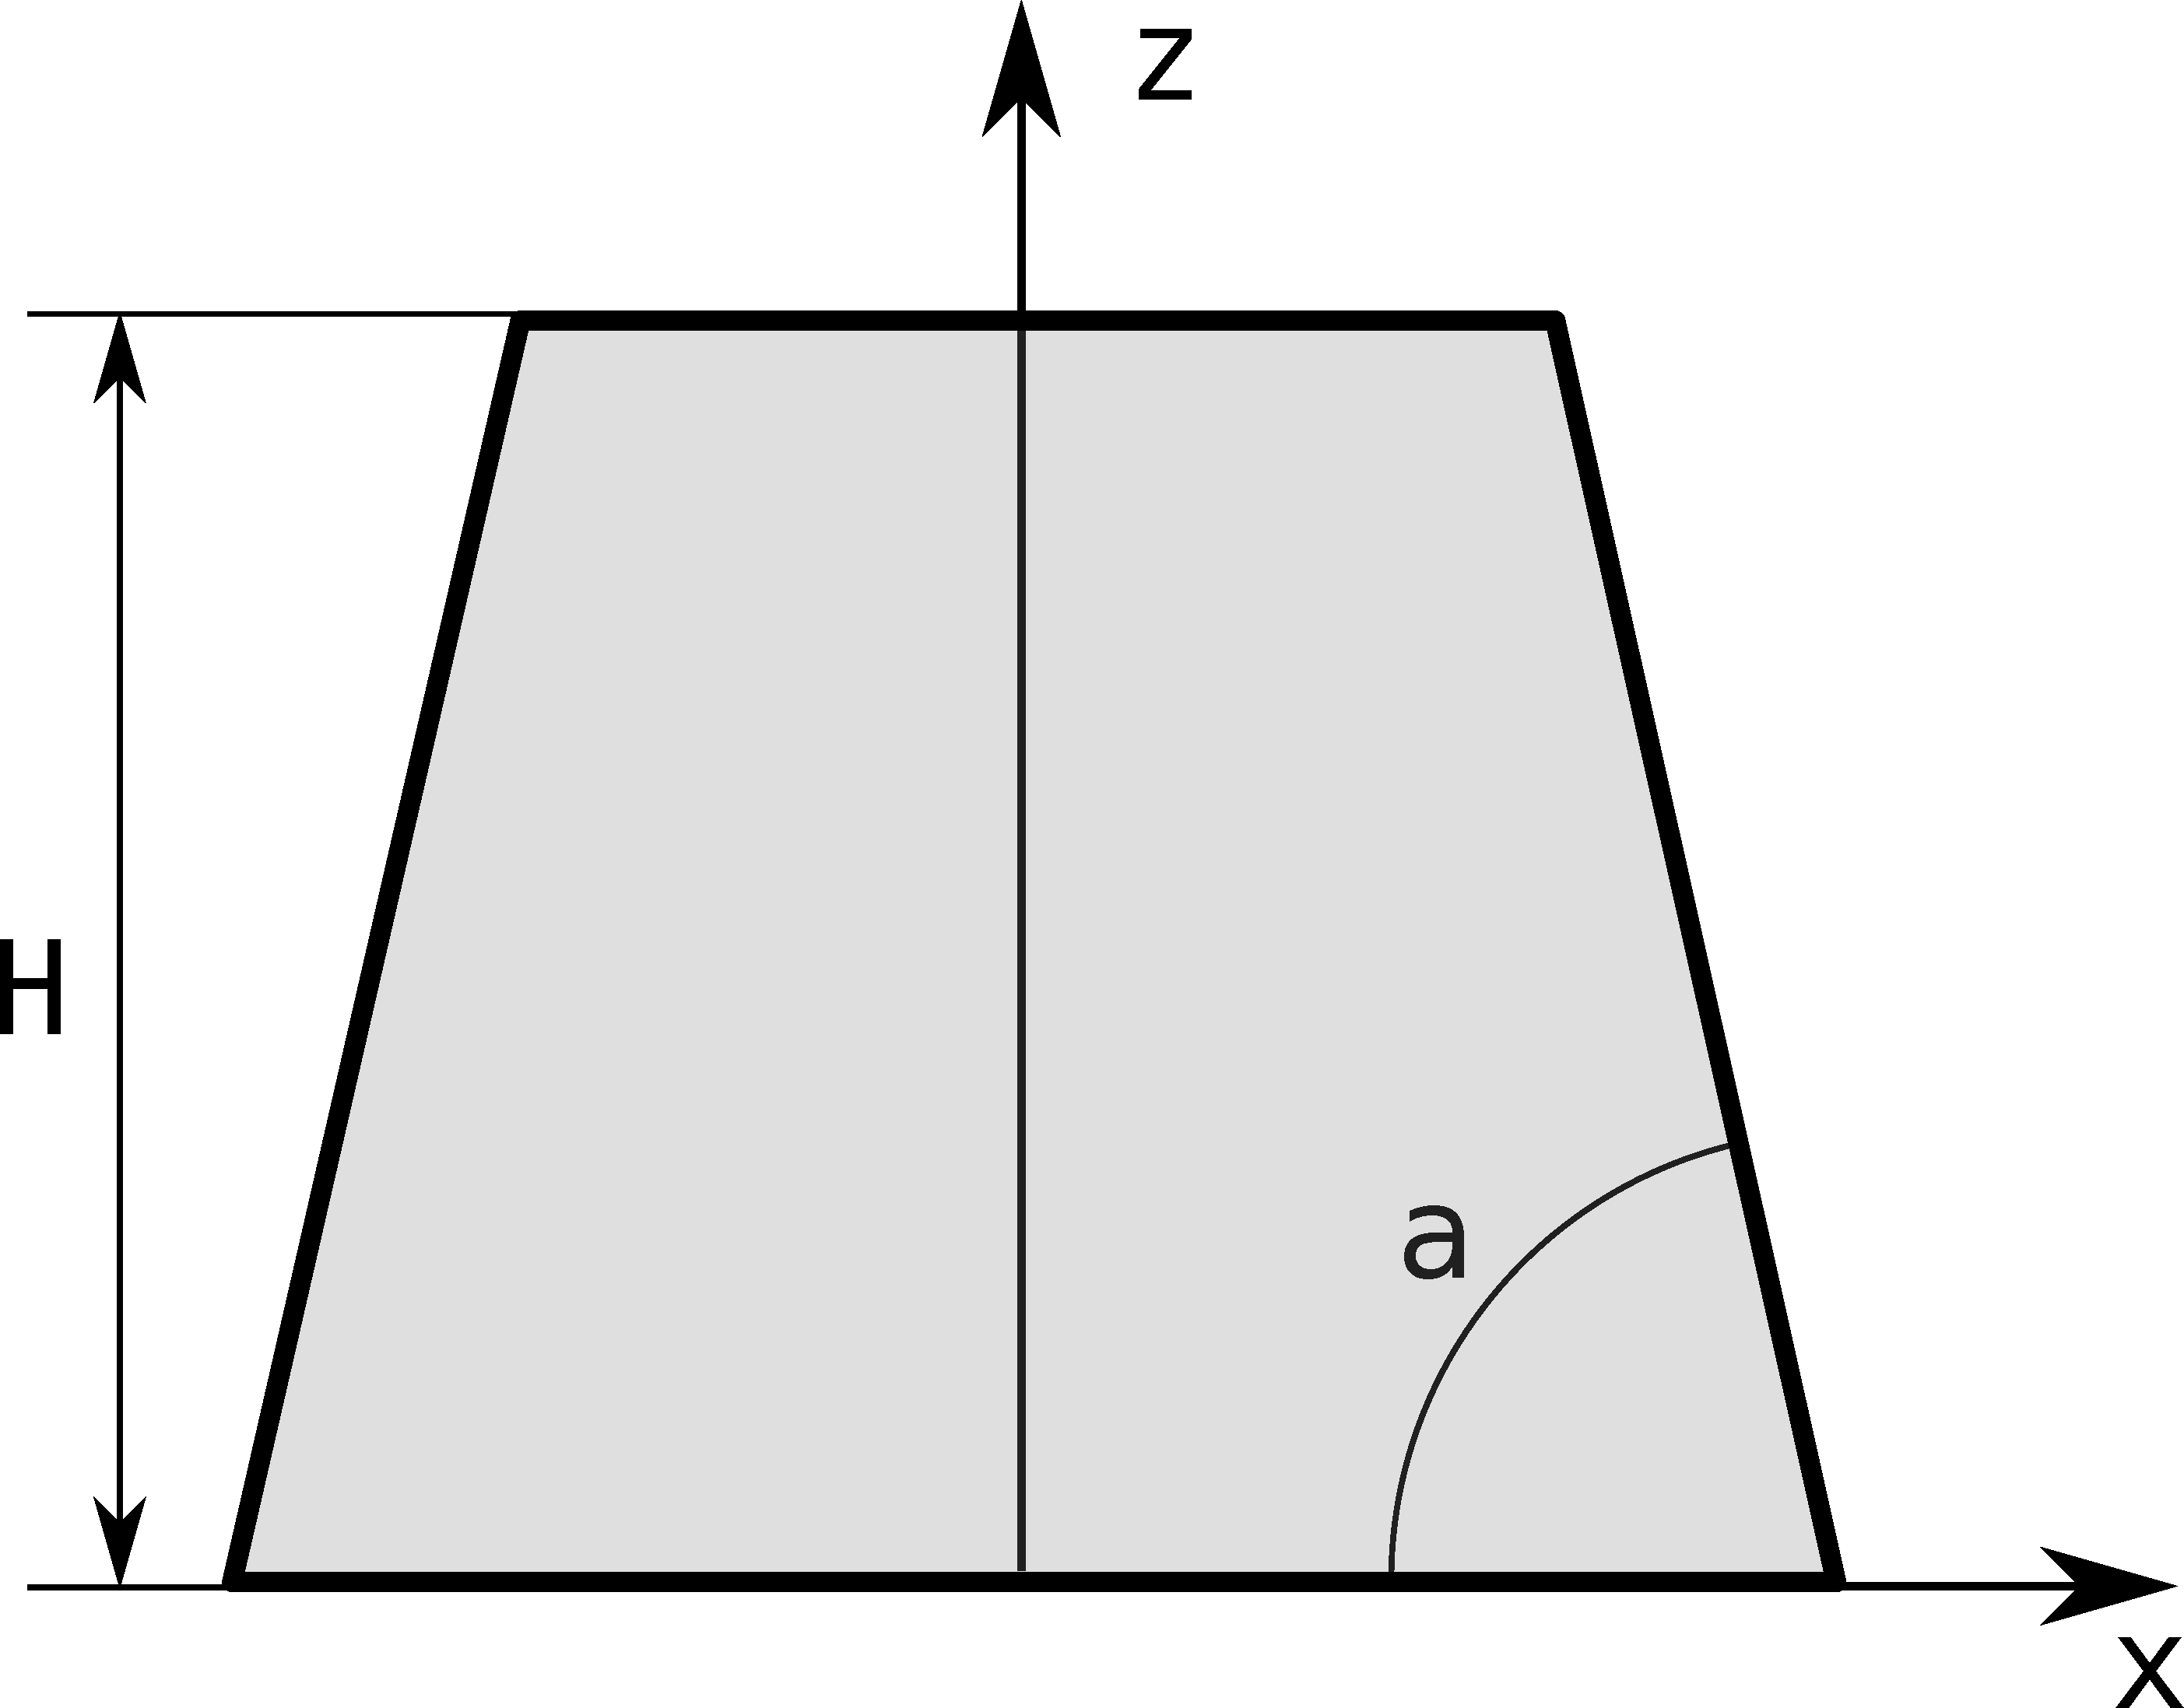
\includegraphics[width=5cm]{fig/cuts/Pyramid2dxz.pdf}}
\hfill
\subfigure[Top view]{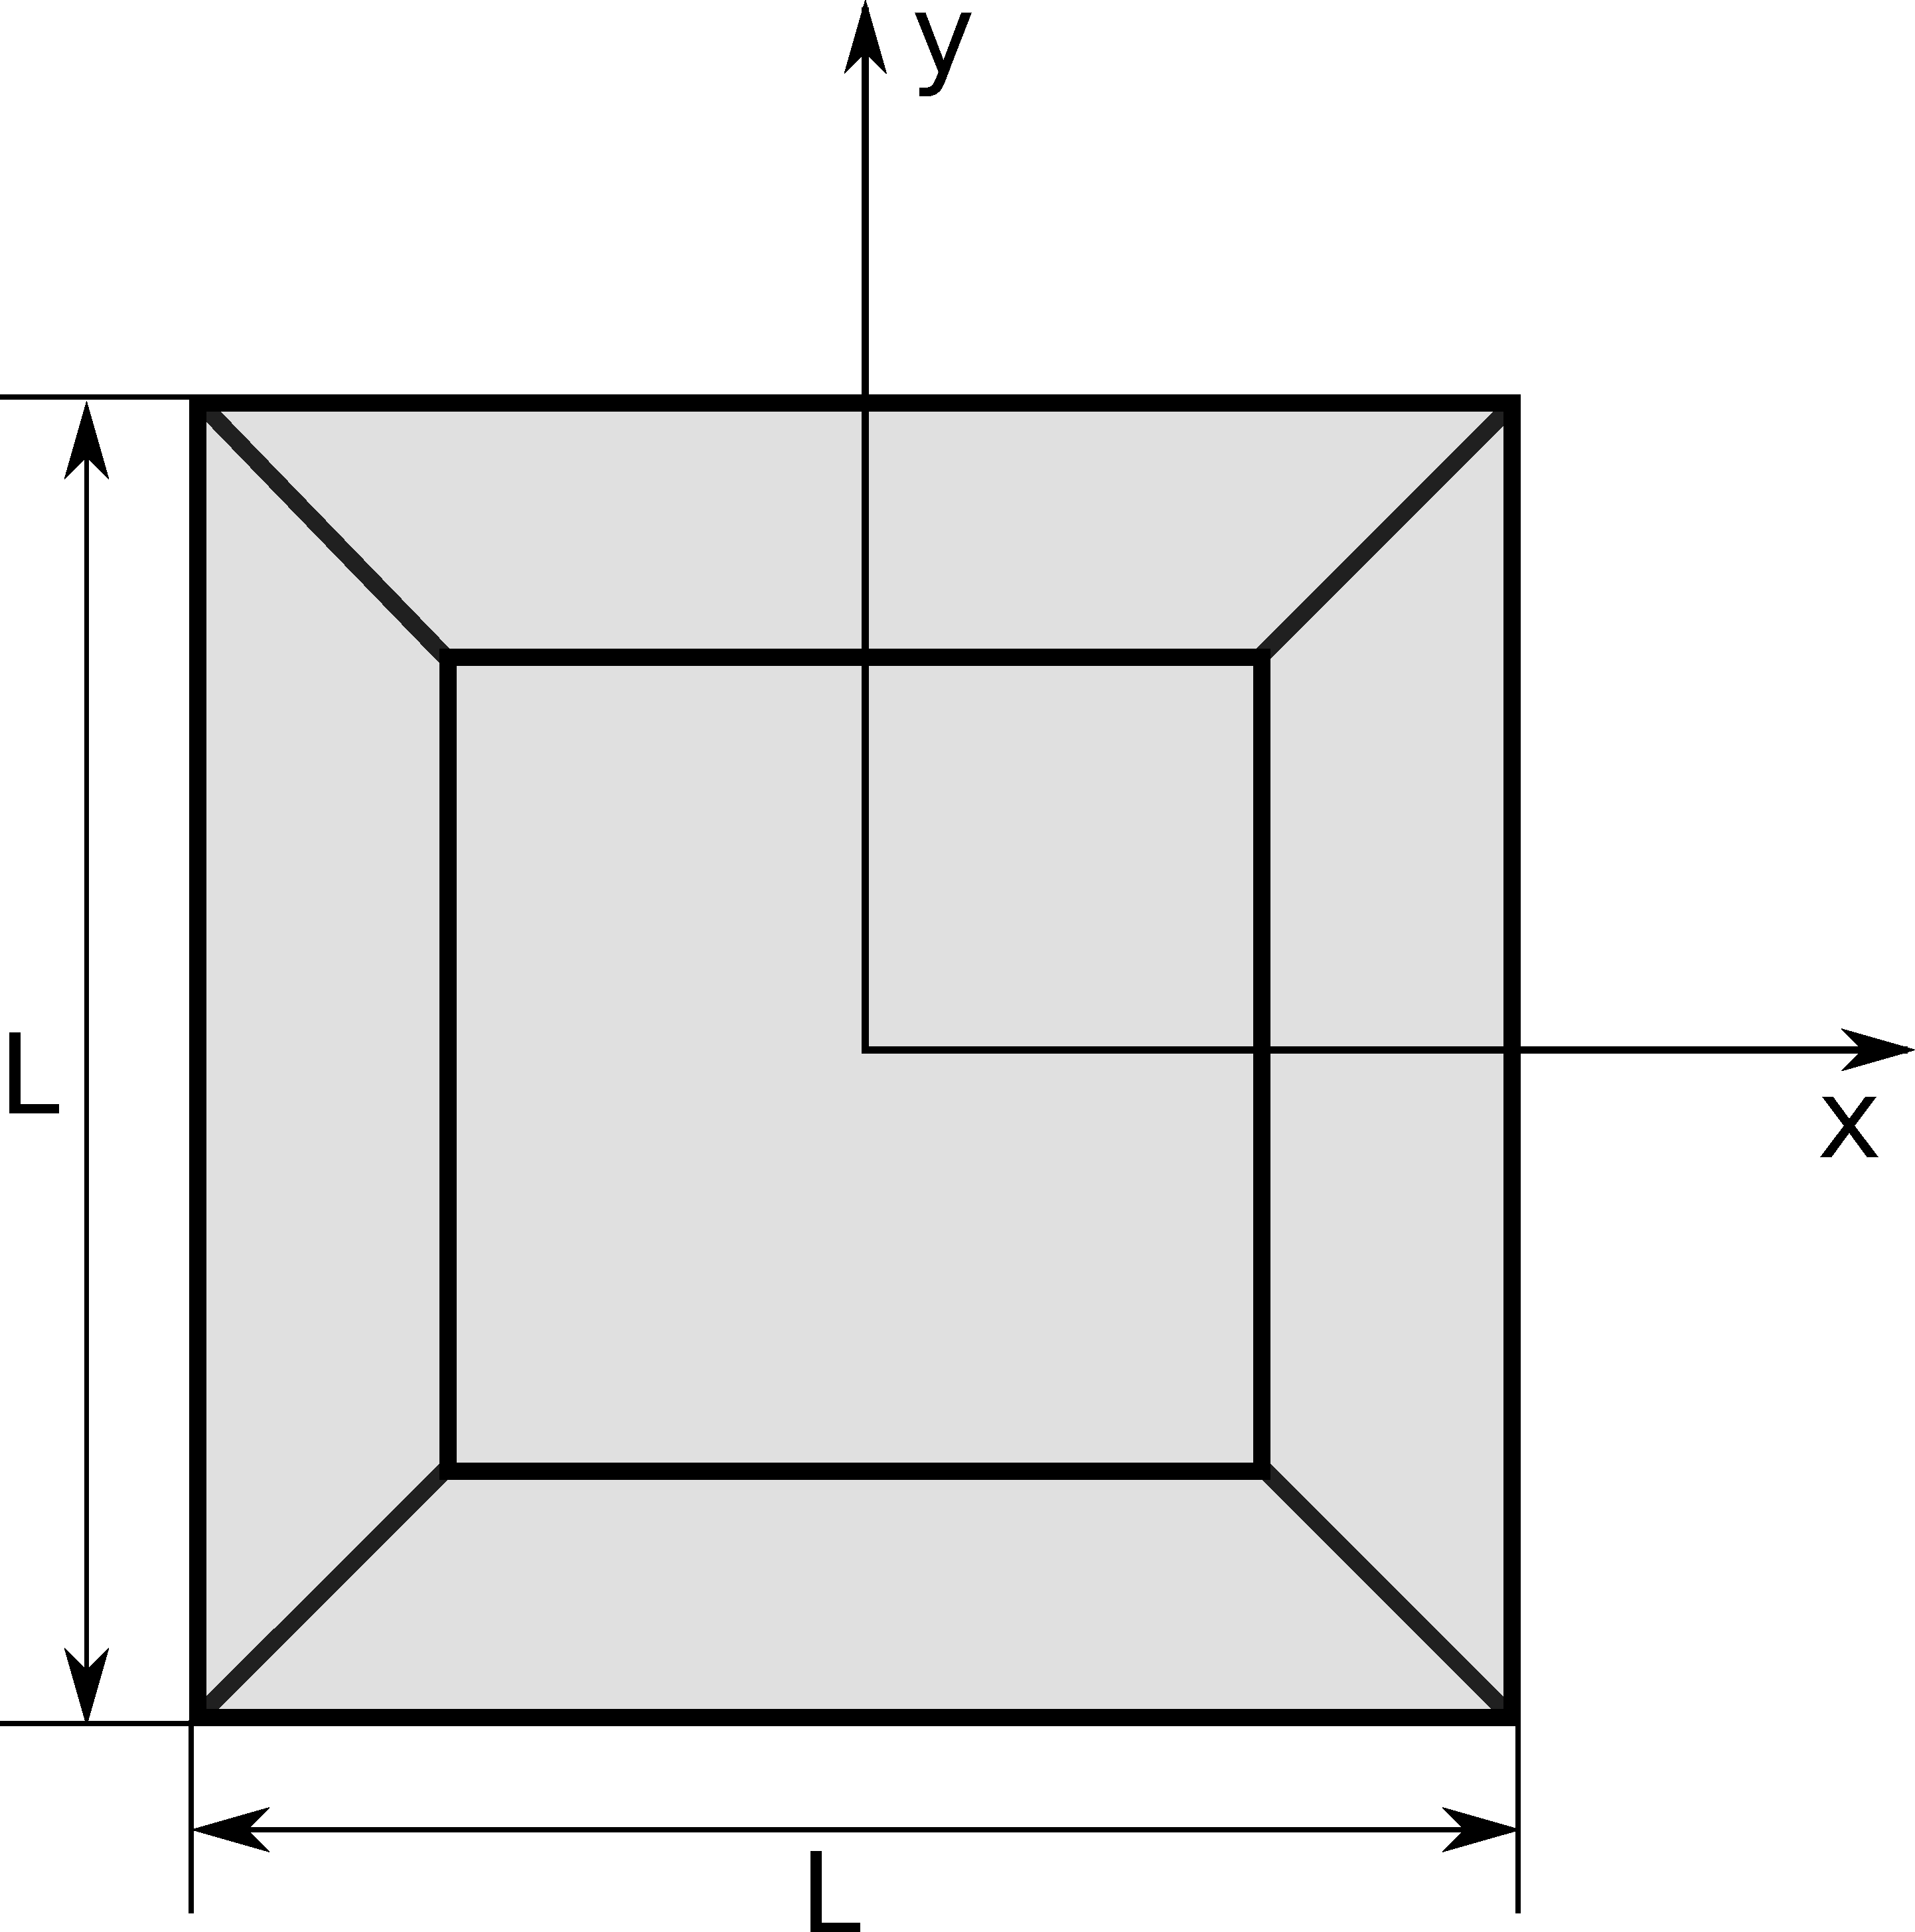
\includegraphics[width=5cm]{fig/cuts/Pyramid2dxy.pdf}}
\hfill
\caption{Sketch of a Pyramid}
\label{fig:pyramid}
\end{figure}

\FloatBarrier

\paragraph{Parameters}
\begin{itemize}
\item length of one side of the square base $L$,  
\item height $H$,
\item  $\alpha$ is the angle between the base and the
  side faces, taken in the middle of the base lines.
\end{itemize}

\paragraph{Restrictions on the parameters:}  $\dfrac{2H}{L} < \tan(\alpha)$.

\paragraph{Properties}
\begin{itemize}
\item  volume $V = \dfrac{1}{6} \tan(\alpha) L^3\left[ 1
             - \left(1 - \dfrac{2H}{\tan(\alpha)L}\right)^3 \right],$
\item particle surface seen from above $S = L^2$.
\end{itemize}

\paragraph{Form factor}
\begin{align*}
&F(\mathbf{q},L, H, \alpha) =
\frac{H}{q_x q_y} \times \nonumber \\ &\left\{ K_1 \cos\left[
  (q_x-q_y)\frac{L}{2} \right] + K_2 \sin\left[ (q_x-q_y)\frac{L}{2} \right]
- K_3 \cos\left[ (q_x+q_y) \frac{L}{2} \right] - K_4 \sin\left[ (q_x+q_y)\frac{L}{2} \right]\right\},
\end{align*}
with $\sinc(x)=\sin(x)/x$,
\begin{align*}
       q_1 &=\frac{1}{2}\Big[\frac{q_x-q_y}{\tan(\alpha)} + q_z\Big],\quad       q_2 =\frac{1}{2}\Big[\frac{q_x-q_y}{\tan(\alpha)} - q_z\Big]\\
        q_3 &=\frac{1}{2}\Big[\frac{q_x+q_y}{\tan(\alpha)} + q_z\Big],\quad       q_4 =\frac{1}{2}\Big[\frac{q_x+q_y}{\tan(\alpha)} - q_z\Big]\\
        K_1 &= \sinc(q_1 H)\exp(i q_1 H)  + \sinc(q_2 H) \exp(-i q_2 H)\\
        K_2 &= -i \sinc(q_1 H) \exp(i q_1 H) +i \sinc(q_2 H) \exp(-i q_2 H)\\
        K_3 &= \sinc(q_3 H) \exp(i q_3 H)    + \sinc(q_4 H) \exp(-i q_4 H)\\
        K_4 &= -i \sinc(q_3 H) \exp(i q_3 H) + i \sinc(q_4 H) \exp(-i q_4 H) 
   \end{align*}

\paragraph{Syntax}\strut\\
\Code{FormFactorPyramid(length, height, alpha)}

\paragraph{Examples}
Figure~\ref{fig:FFPyramidEx} shows the normalized intensity
$|F|^2/V^2$, computed with $L=18$~nm, $H=13$~nm and
$\alpha=60^{\circ}$.

\begin{figure}[ht]
\begin{center}
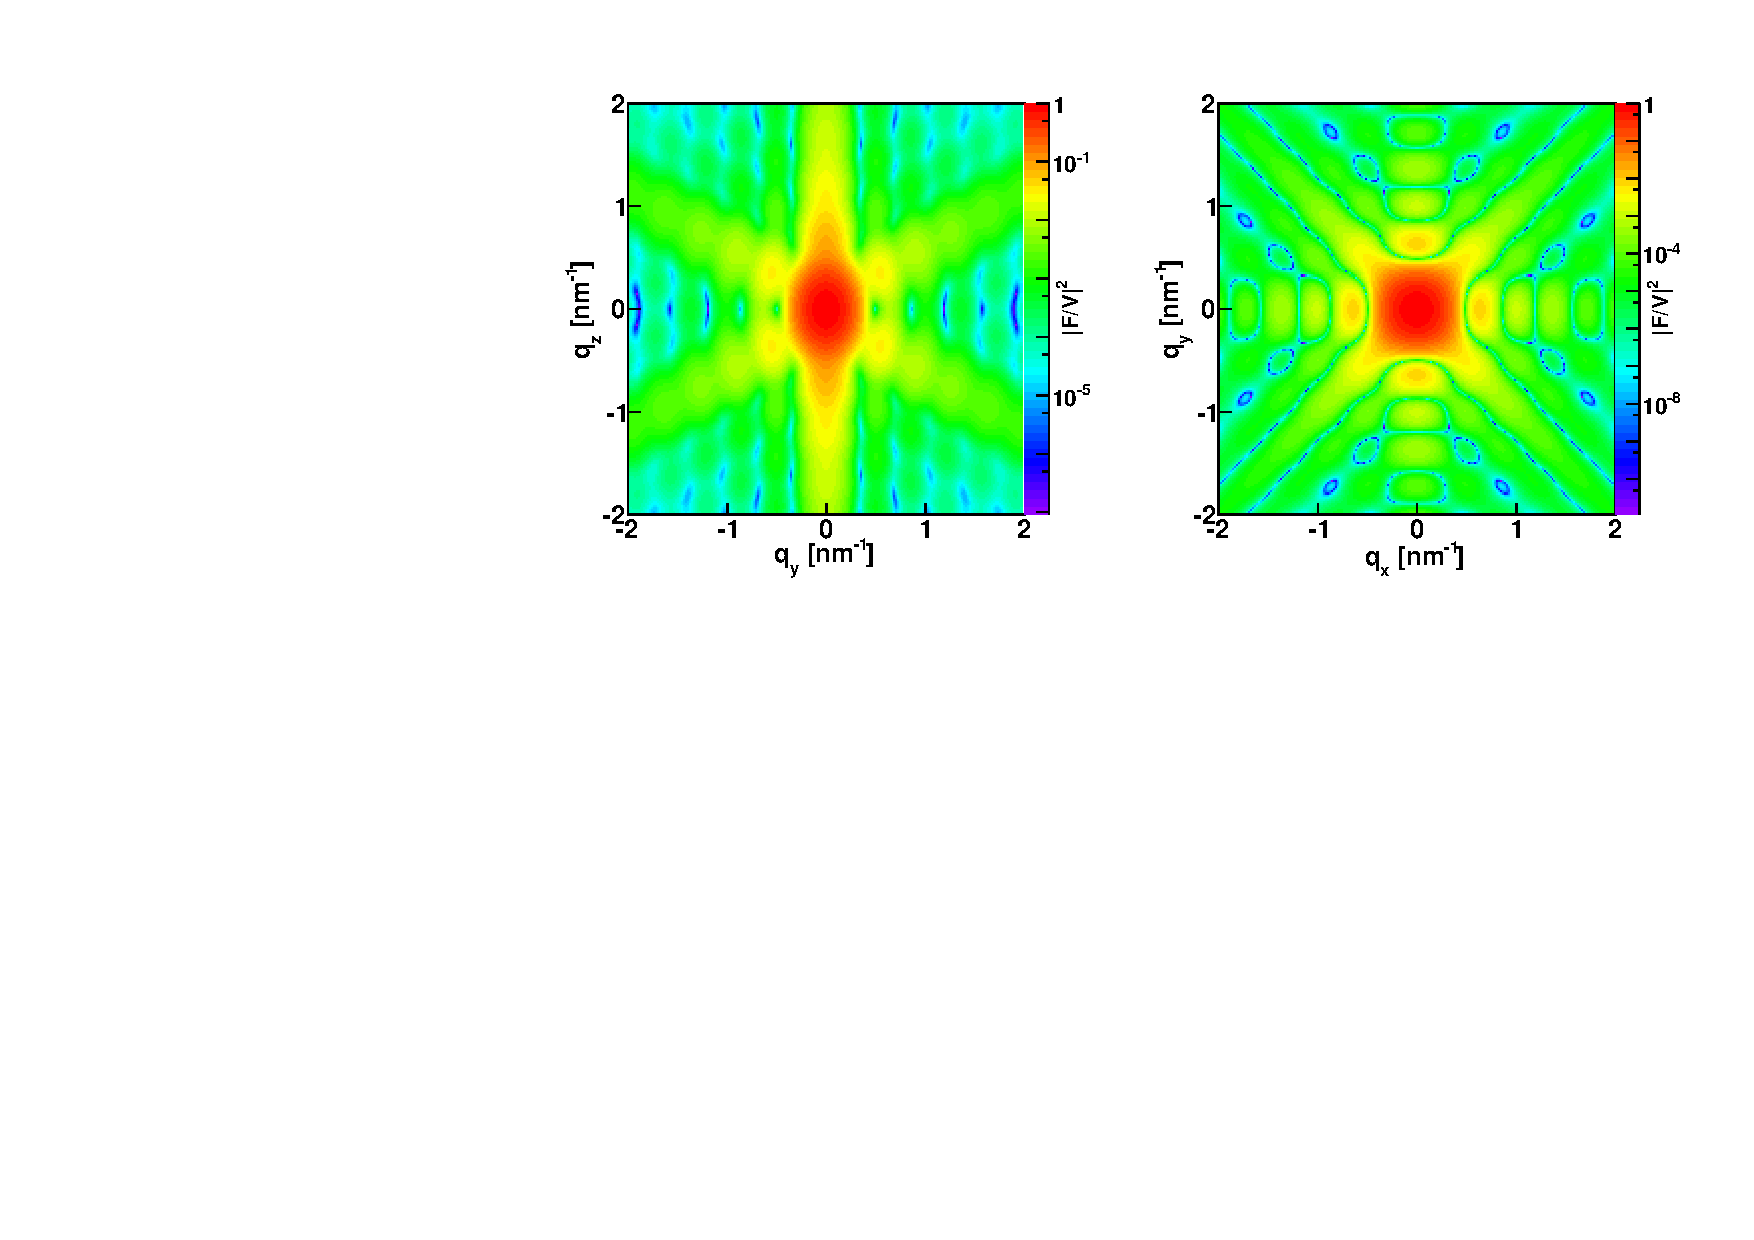
\includegraphics[angle=-90,width=\textwidth]{fig/ff/figffpyramid.pdf}
\end{center}
\caption{Normalized intensity for the form factor of a
  pyramid plotted against ($q_y$, $q_z$) and  
  ($q_x$, $q_y$) and computed with  \Code{FormFactorPyramid(18.*nanometer, 13.*nanometer, 60.*degree)}.}
\label{fig:FFPyramidEx}
\end{figure}

\paragraph{References}\strut\\
Agrees with \lq\lq Pyramid\rq\rq\ form factor of \IsGISAXS~\cite{Laz02},
except for different parametrization $L=2R_{\rm{\Code{IsGISXAXS}}}$.
[and sign problem??]

%-------------------------------------------------------------------------------
\newpage
\subsection{AnisoPyramid (rectangle-based)} \label{sec:AnisoPyramid} 
  \index{Anisotropic pyramid (form factor)}
  \index{Pyramid (form factor)!rectangular (AnisoPyramid)}
  \index{Truncated pyramid (form factor)!rectangular (AnisoPyramid)}
  \index{FormFactorAnisoPyramid@\Code{FormFactorAnisoPyramid}}
%-------------------------------------------------------------------------------

\paragraph{Real-space geometry}\strut\\
A truncated right pyramid with a rectangular base as
shown in fig.~\ref{fig:anisopyramid}.

\begin{figure}[ht]
\hfill
\subfigure[Side view]{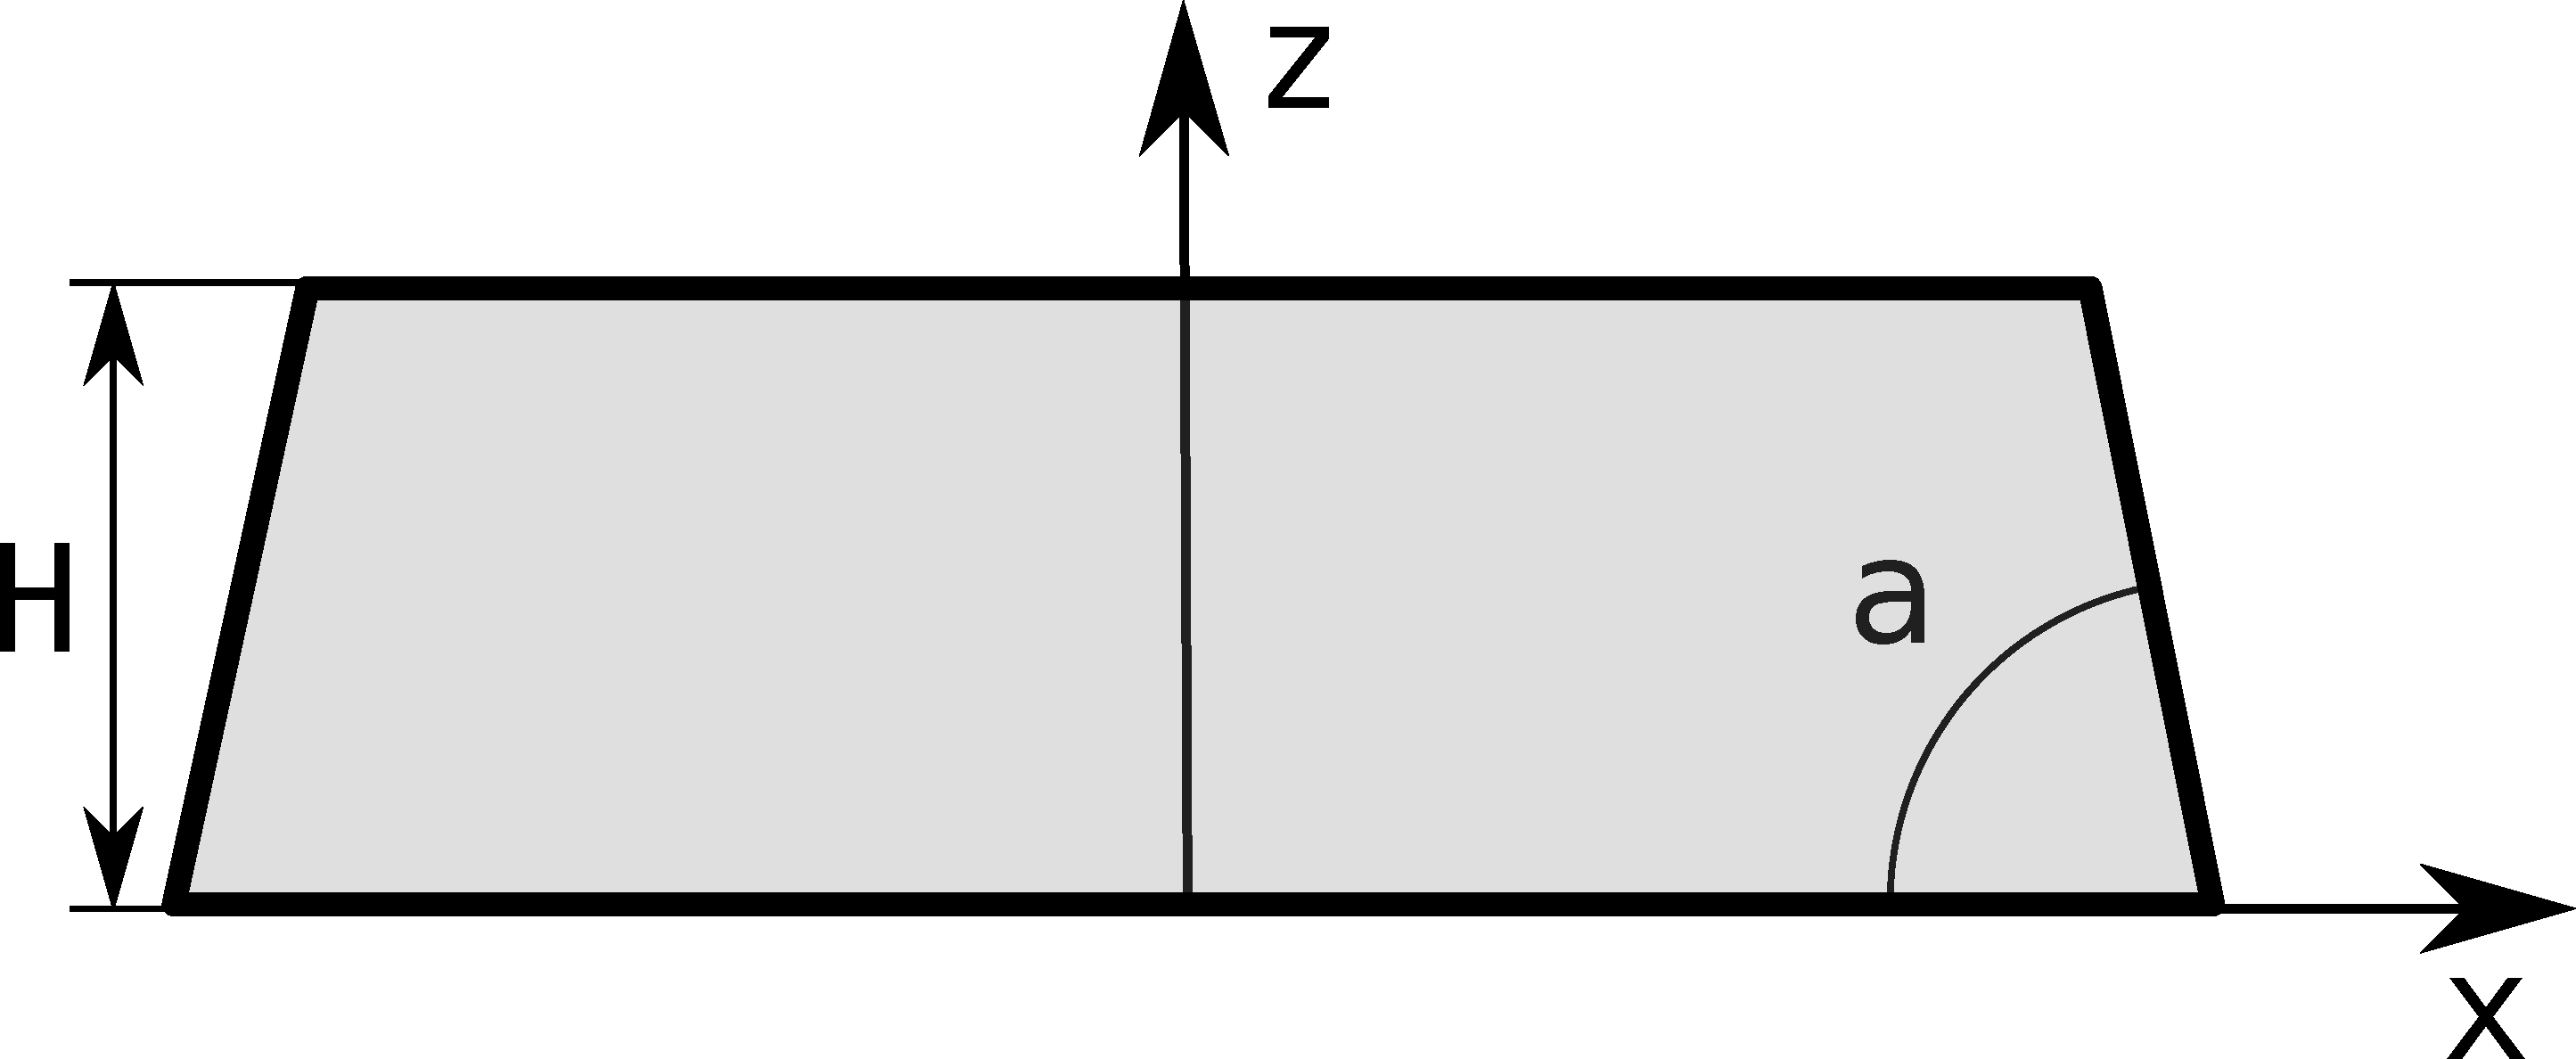
\includegraphics[width=5cm]{fig/cuts/AnisoPyramid2dxz.pdf}}
\hfill
\subfigure[Top view]{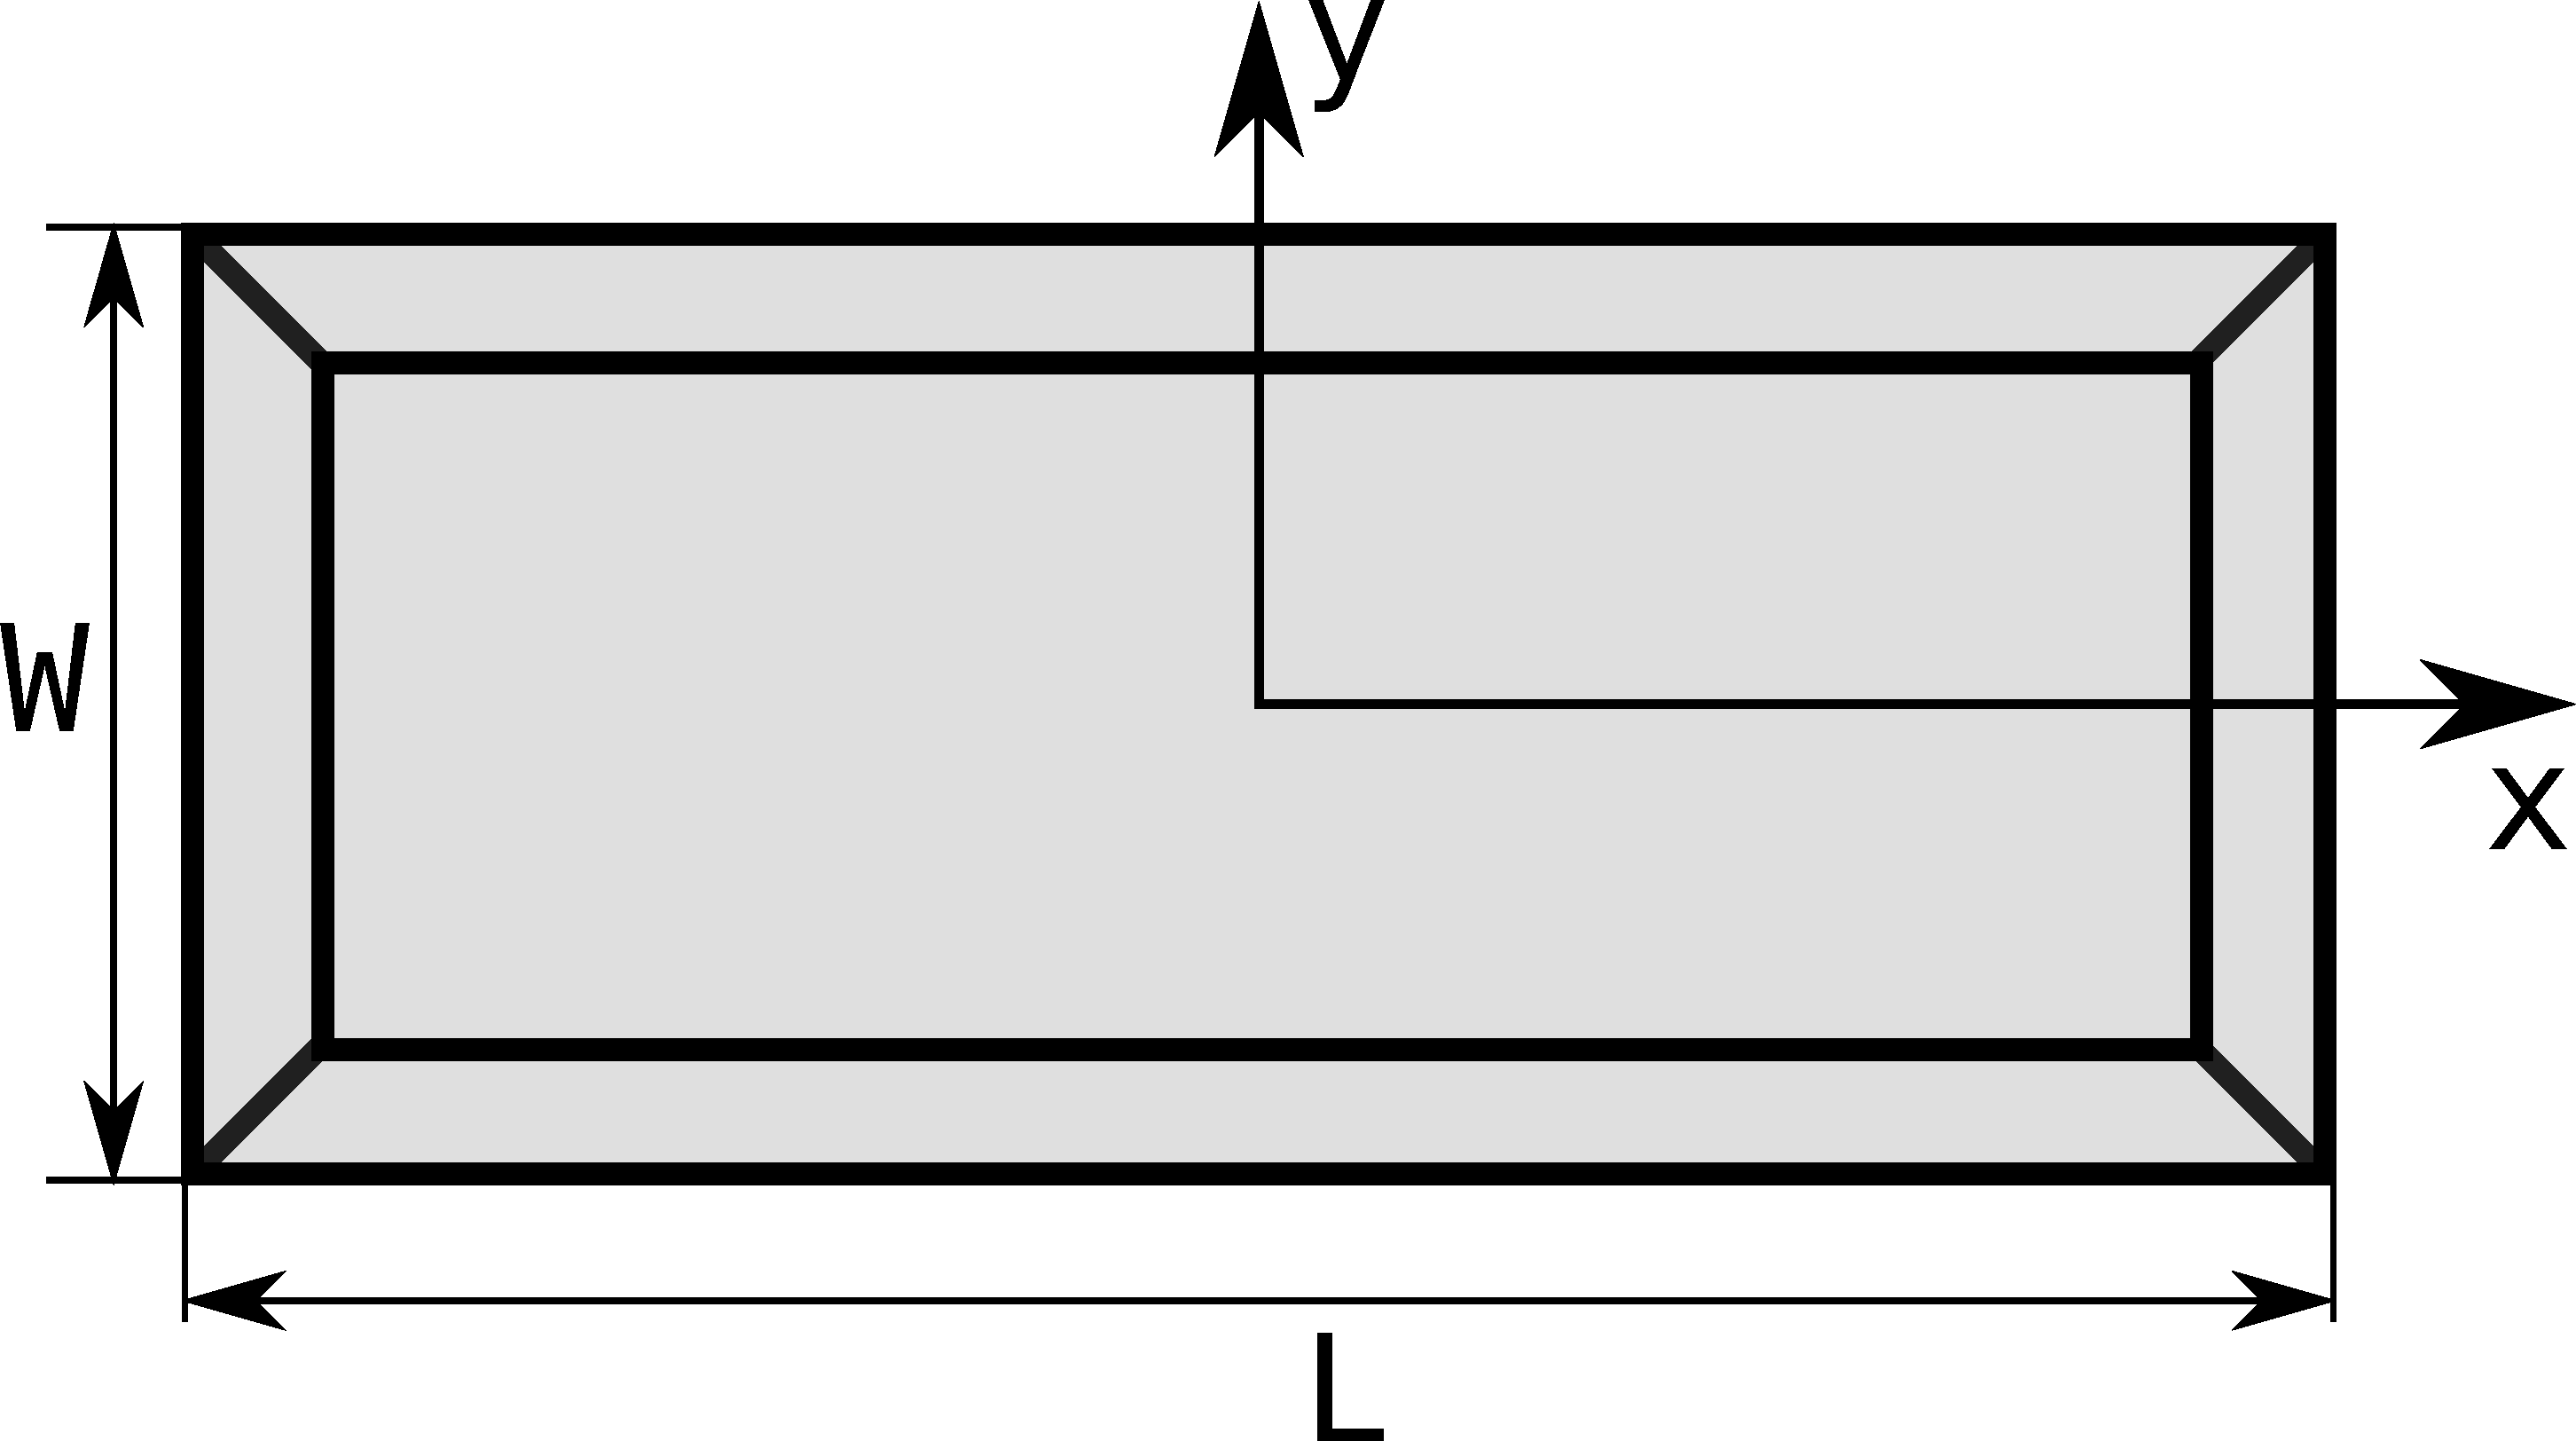
\includegraphics[width=5cm]{fig/cuts/AnisoPyramid2dxy.pdf}}
\hfill
\caption{Sketch of an Anisotropic Pyramid.}
\label{fig:anisopyramid}
\end{figure}

\FloatBarrier

\paragraph{Parameters}
\begin{itemize}
\item full length of the base $L$,
\item full width of the base $W$,
\item height $H$,
\item $\alpha$ is the angle between the base and the
  side faces, taken in the middle of the base lines.
\end{itemize}

\paragraph{Restrictions on the parameters:} $\dfrac{2H}{L}< \tan(\alpha)$ and $\dfrac{2H}{W}< \tan(\alpha)$.

\paragraph{Properties}
\begin{itemize}
\item volume $V= H \Big[LW - \dfrac{(L + W)H}{\tan(\alpha)}
   + \dfrac{4}{3} \dfrac{H^2}{\tan^2(\alpha)}\Big]$,
\item particle surface seen from above $S = LW$.
\end{itemize}

\paragraph{Form factor}
\begin{align*}
&F(\mathbf{q}, L, W, H, \alpha)=
\frac{H}{q_xq_y} \times \\
&\Big\{
K_1\cos\Big(q_x \frac{L}{2} -q_y \frac{W}{2}\Big)+  K_2 \sin \Big (q_x
\frac{L}{2}- q_y \frac{W}{2}\Big) - K_3 \cos \Big (q_x \frac{L}{2} +q_y \frac{W}{2}\Big)-
K_4 \sin \Big (q_x \frac{L}{2} + q_y \frac{W}{2}\Big)
\Big\},
\end{align*}
with $\sinc(x)=\sin(x)/x$,
\begin{align*}
K_1 &= \exp(-i q_2 H) \sinc(q_2 H) + \exp(iq_1 H) \sinc(q_1 H) \\
K_2 &= i \exp(-iq_2 H) \sinc(q_2 H) -i \exp(iq_1 H) \sinc(q_1 H) \\
K_3 &= \exp(-iq_4 H) \sinc(q_4 H) + \exp(iq_3 H) \sinc(q_3 H) \\
K_4 &= i \exp(i q_4 H) \sinc(q_4 H) -i \exp(iq_3 H) \sinc(q_3 H)\\
q_1 &= \frac{1}{2}\left[\frac{q_x -q_y}{\tan \alpha} +q_z \right],\quad q_2 = \frac{1}{2}\left[\frac{q_x -q_y}{\tan \alpha} -q_z \right]\\
q_3 &= \frac{1}{2}\left[\frac{q_x +q_y}{\tan \alpha} +q_z \right] , \quad q_4 = \frac{1}{2}\left[\frac{q_x +q_y}{\tan \alpha} -q_z \right]
\end{align*}

\paragraph{Syntax}\strut\\
\Code{FormFactorAnisoPyramid(length, width, height, alpha)}

\paragraph{Example}\strut\\
Figure~\ref{fig:FFAnisoPyramidEx} shows the normalized intensity
$|F|^2/V^2$, computed with $L=20$~nm, $W=16$~nm, $H=13$~nm, and
$\alpha=60^{\circ}$.

\begin{figure}[ht]
\begin{center}
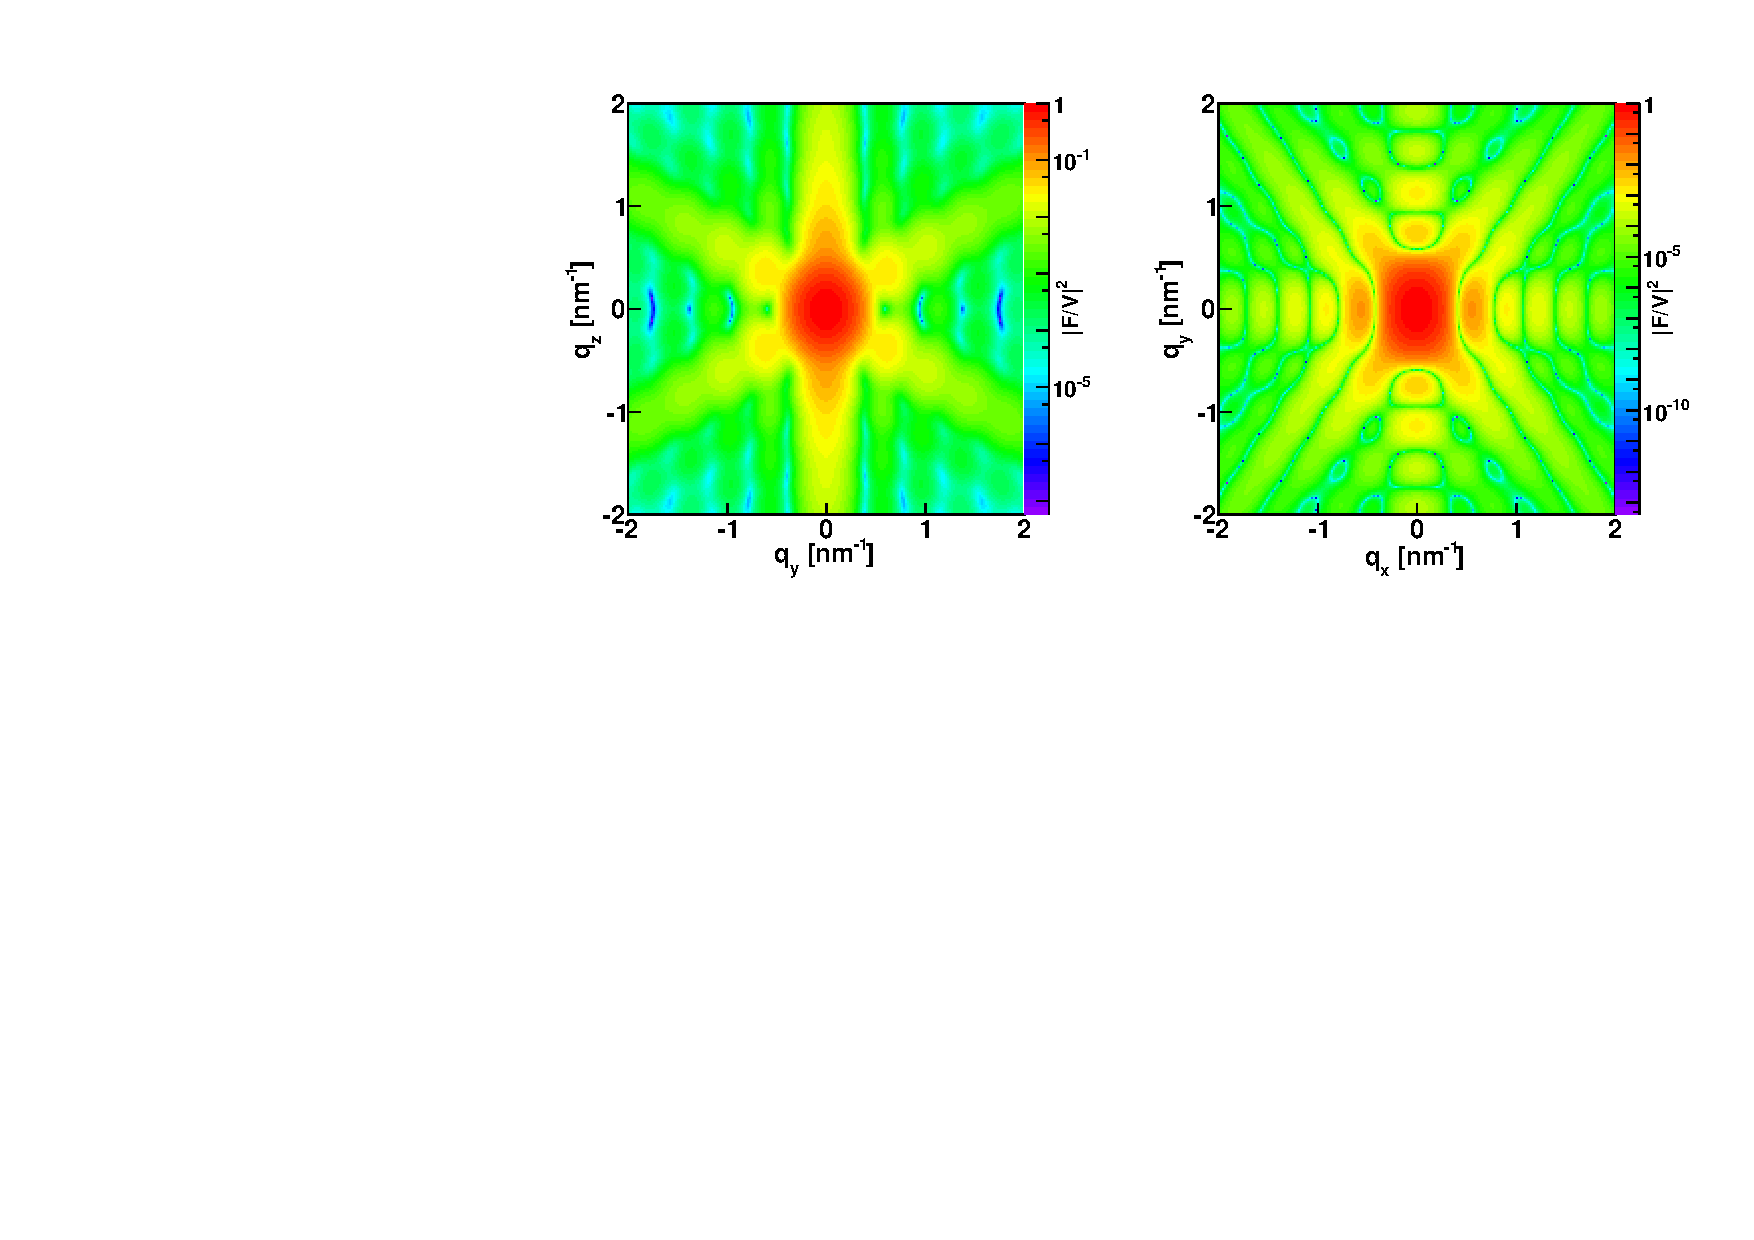
\includegraphics[angle=-90,width=\textwidth]{fig/ff/figffanisopyramid.pdf}
\end{center}
\caption{Normalized intensity for the form factor of an anisotropic
  pyramid $|F|^2/V^2$, plotted against ($q_y$, $q_z$) and  ($q_x$, $q_y$) and computed with \Code{FormFactorAnisoPyramid(20.*nanometer, 16.*nanometer, 13.*nanometer, 60.*degree)}.}
\label{fig:FFAnisoPyramidEx}
\end{figure}

\paragraph{References}\strut\\
Agrees with \lq\lq AnisoPyramid\rq\rq\ form factor of \IsGISAXS~\cite{Laz02},
except for different parametrization. ???

%\subsection{References}
%Like in \Code{IsGISAXS}, the base angle $\alpha$ is the same for both unequal
%side. This means that a full anisotropic pyramid is not a limit case. \\
%But \BornAgain\ uses a different convention of the parameters relative
%to the base. We input the full length and width instead of half values.
%Condition on the parameters: 
%Should not it be: H/R < tan(alpha) and  H/W < tan(alpha) instead of H/R < tan(alpha) and  
%W/R < tan(alpha) where H is the height and R, W the side-lengths of the rectangular base?

%-------------------------------------------------------------------------------
\newpage
\subsection{Cuboctahedron} \label{sec:Cuboctahedron}
  \index{Cuboctahedron (form factor)}
  \index{FormFactorCuboctahedron@\Code{FormFactorCuboctahedron}}
%-------------------------------------------------------------------------------

\paragraph{Real-space geometry}\strut\\
It is a combination of two pyramids with square bases, as shown in fig.~\ref{fig:cuboctahedron}: the bottom one
is upside down with an height $H$ and the top one has the opposite
orientation (the standard one) and an height $r_H \times H$.

\begin{figure}[ht]
\hfill
\subfigure[Side view]{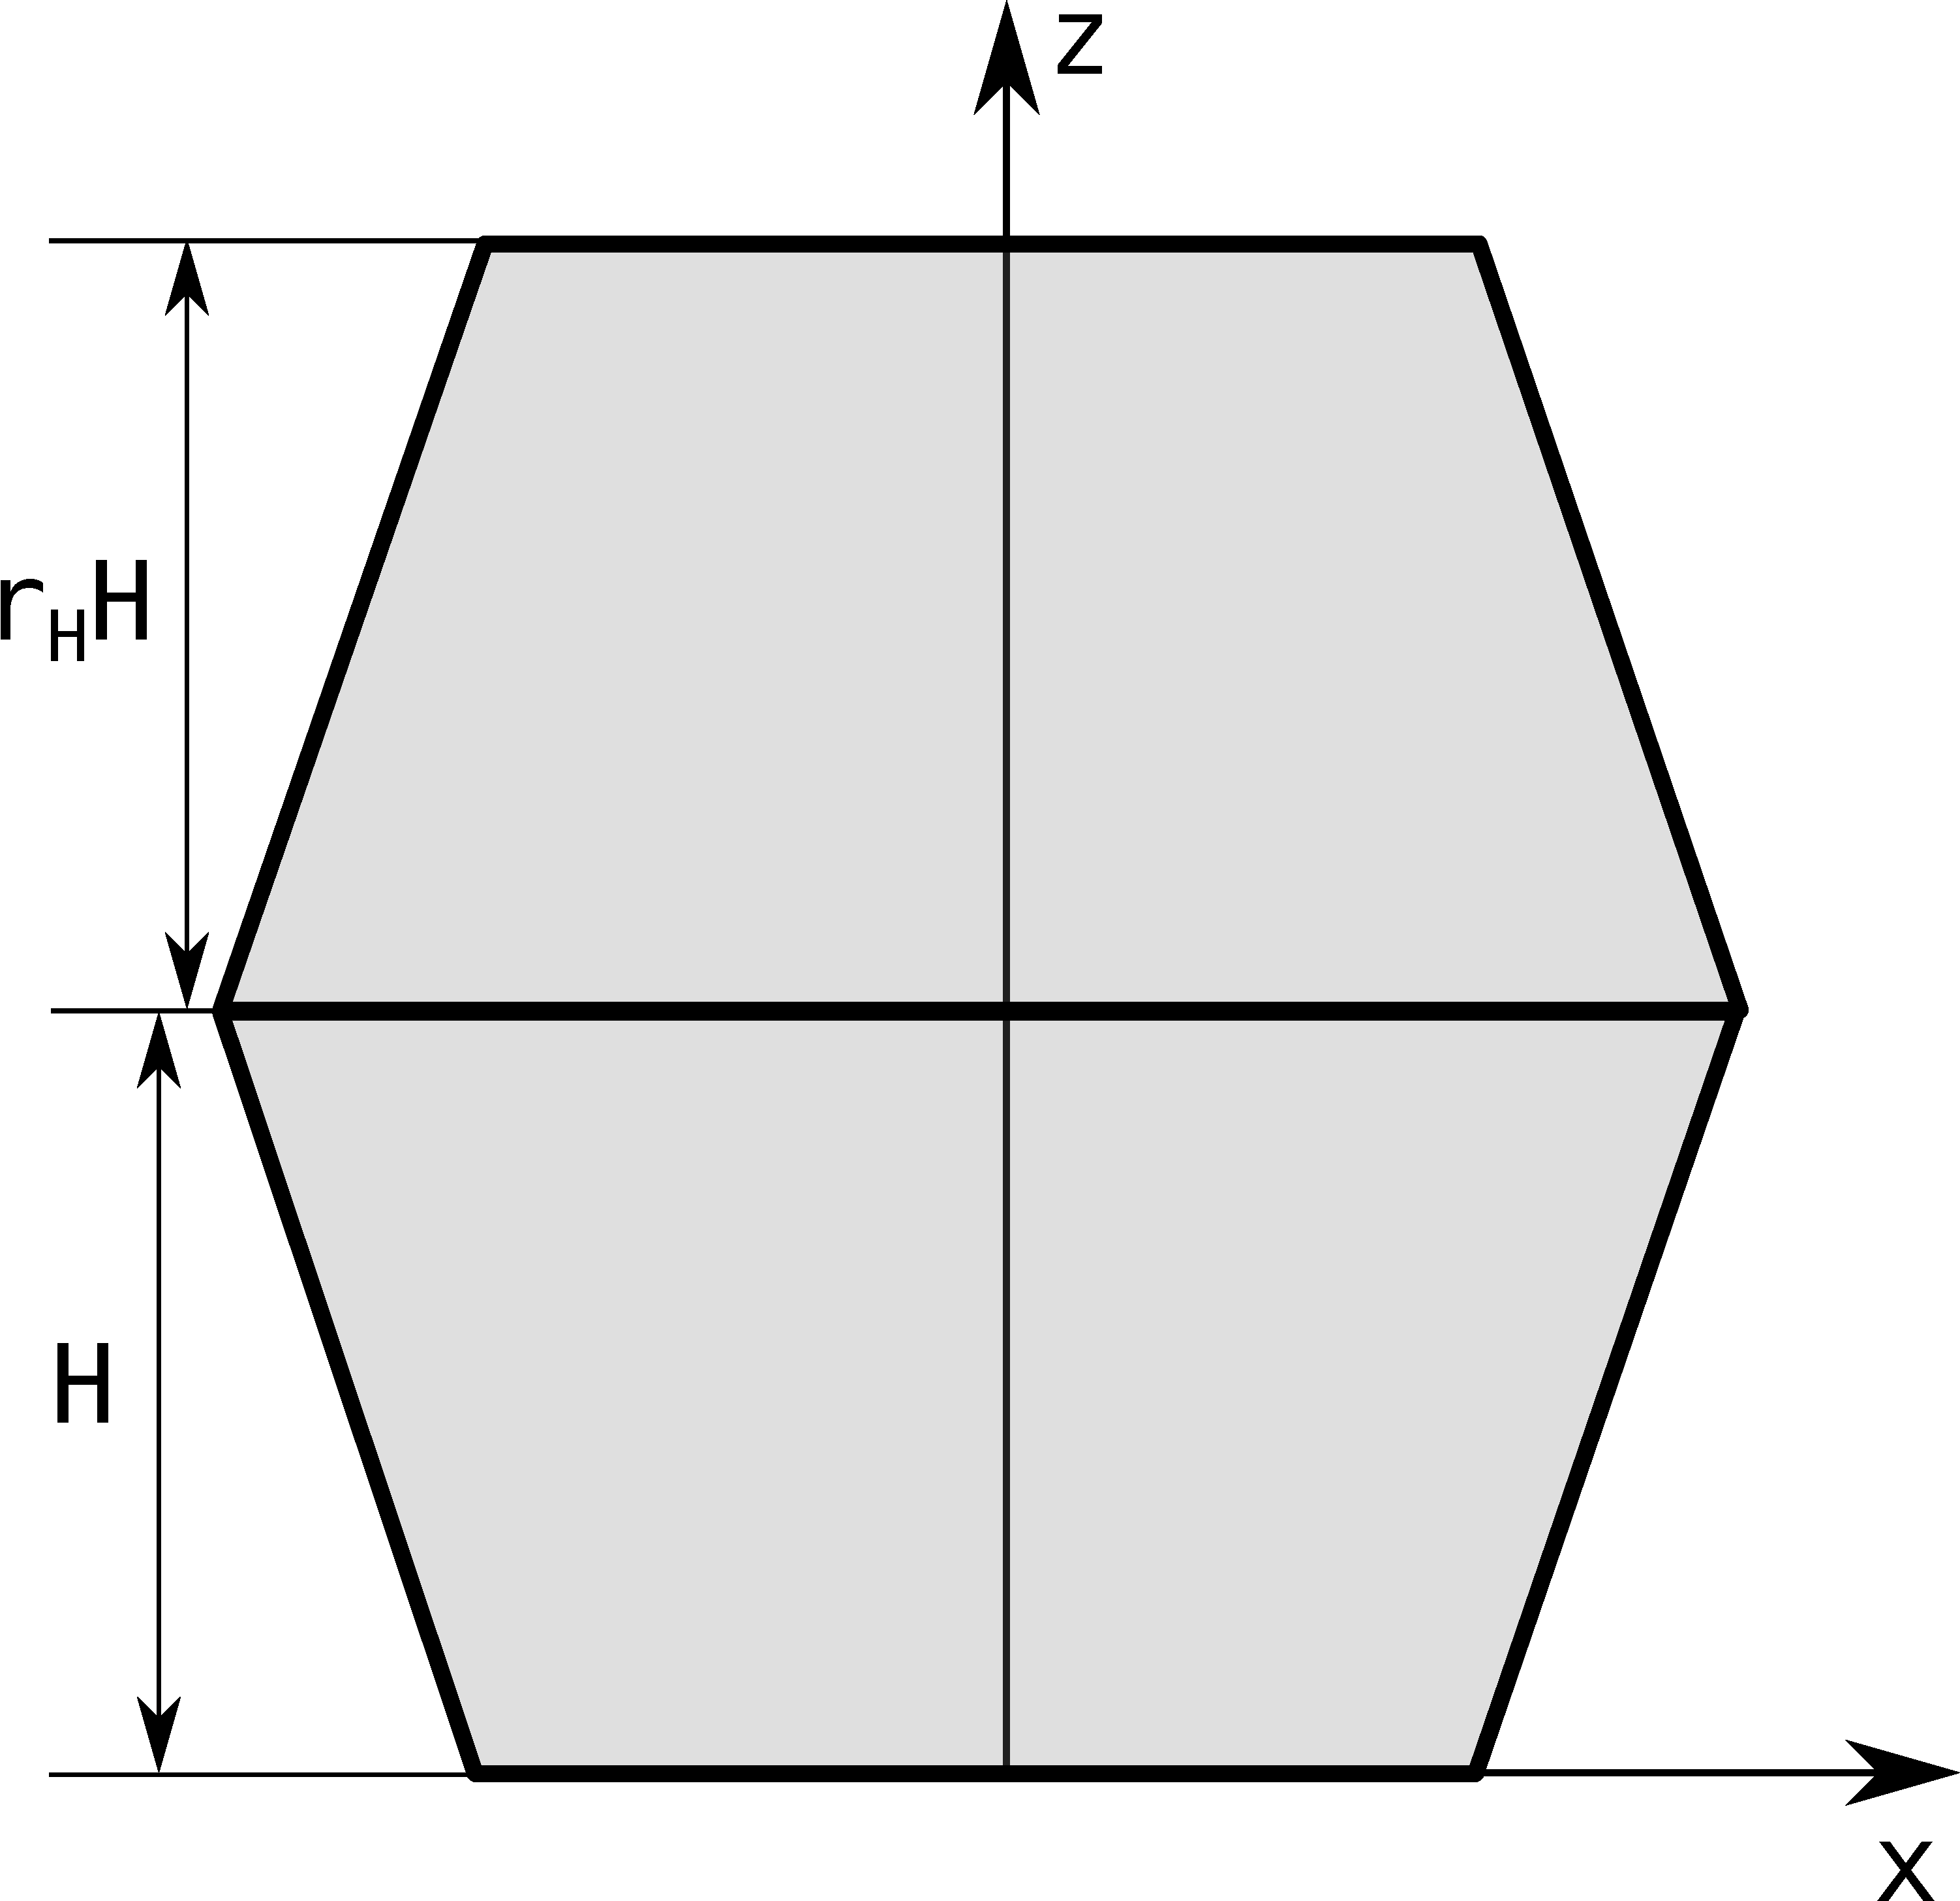
\includegraphics[width=5cm]{fig/cuts/Cuboctahedron2dxz.pdf}}
\hfill
\subfigure[Top view]{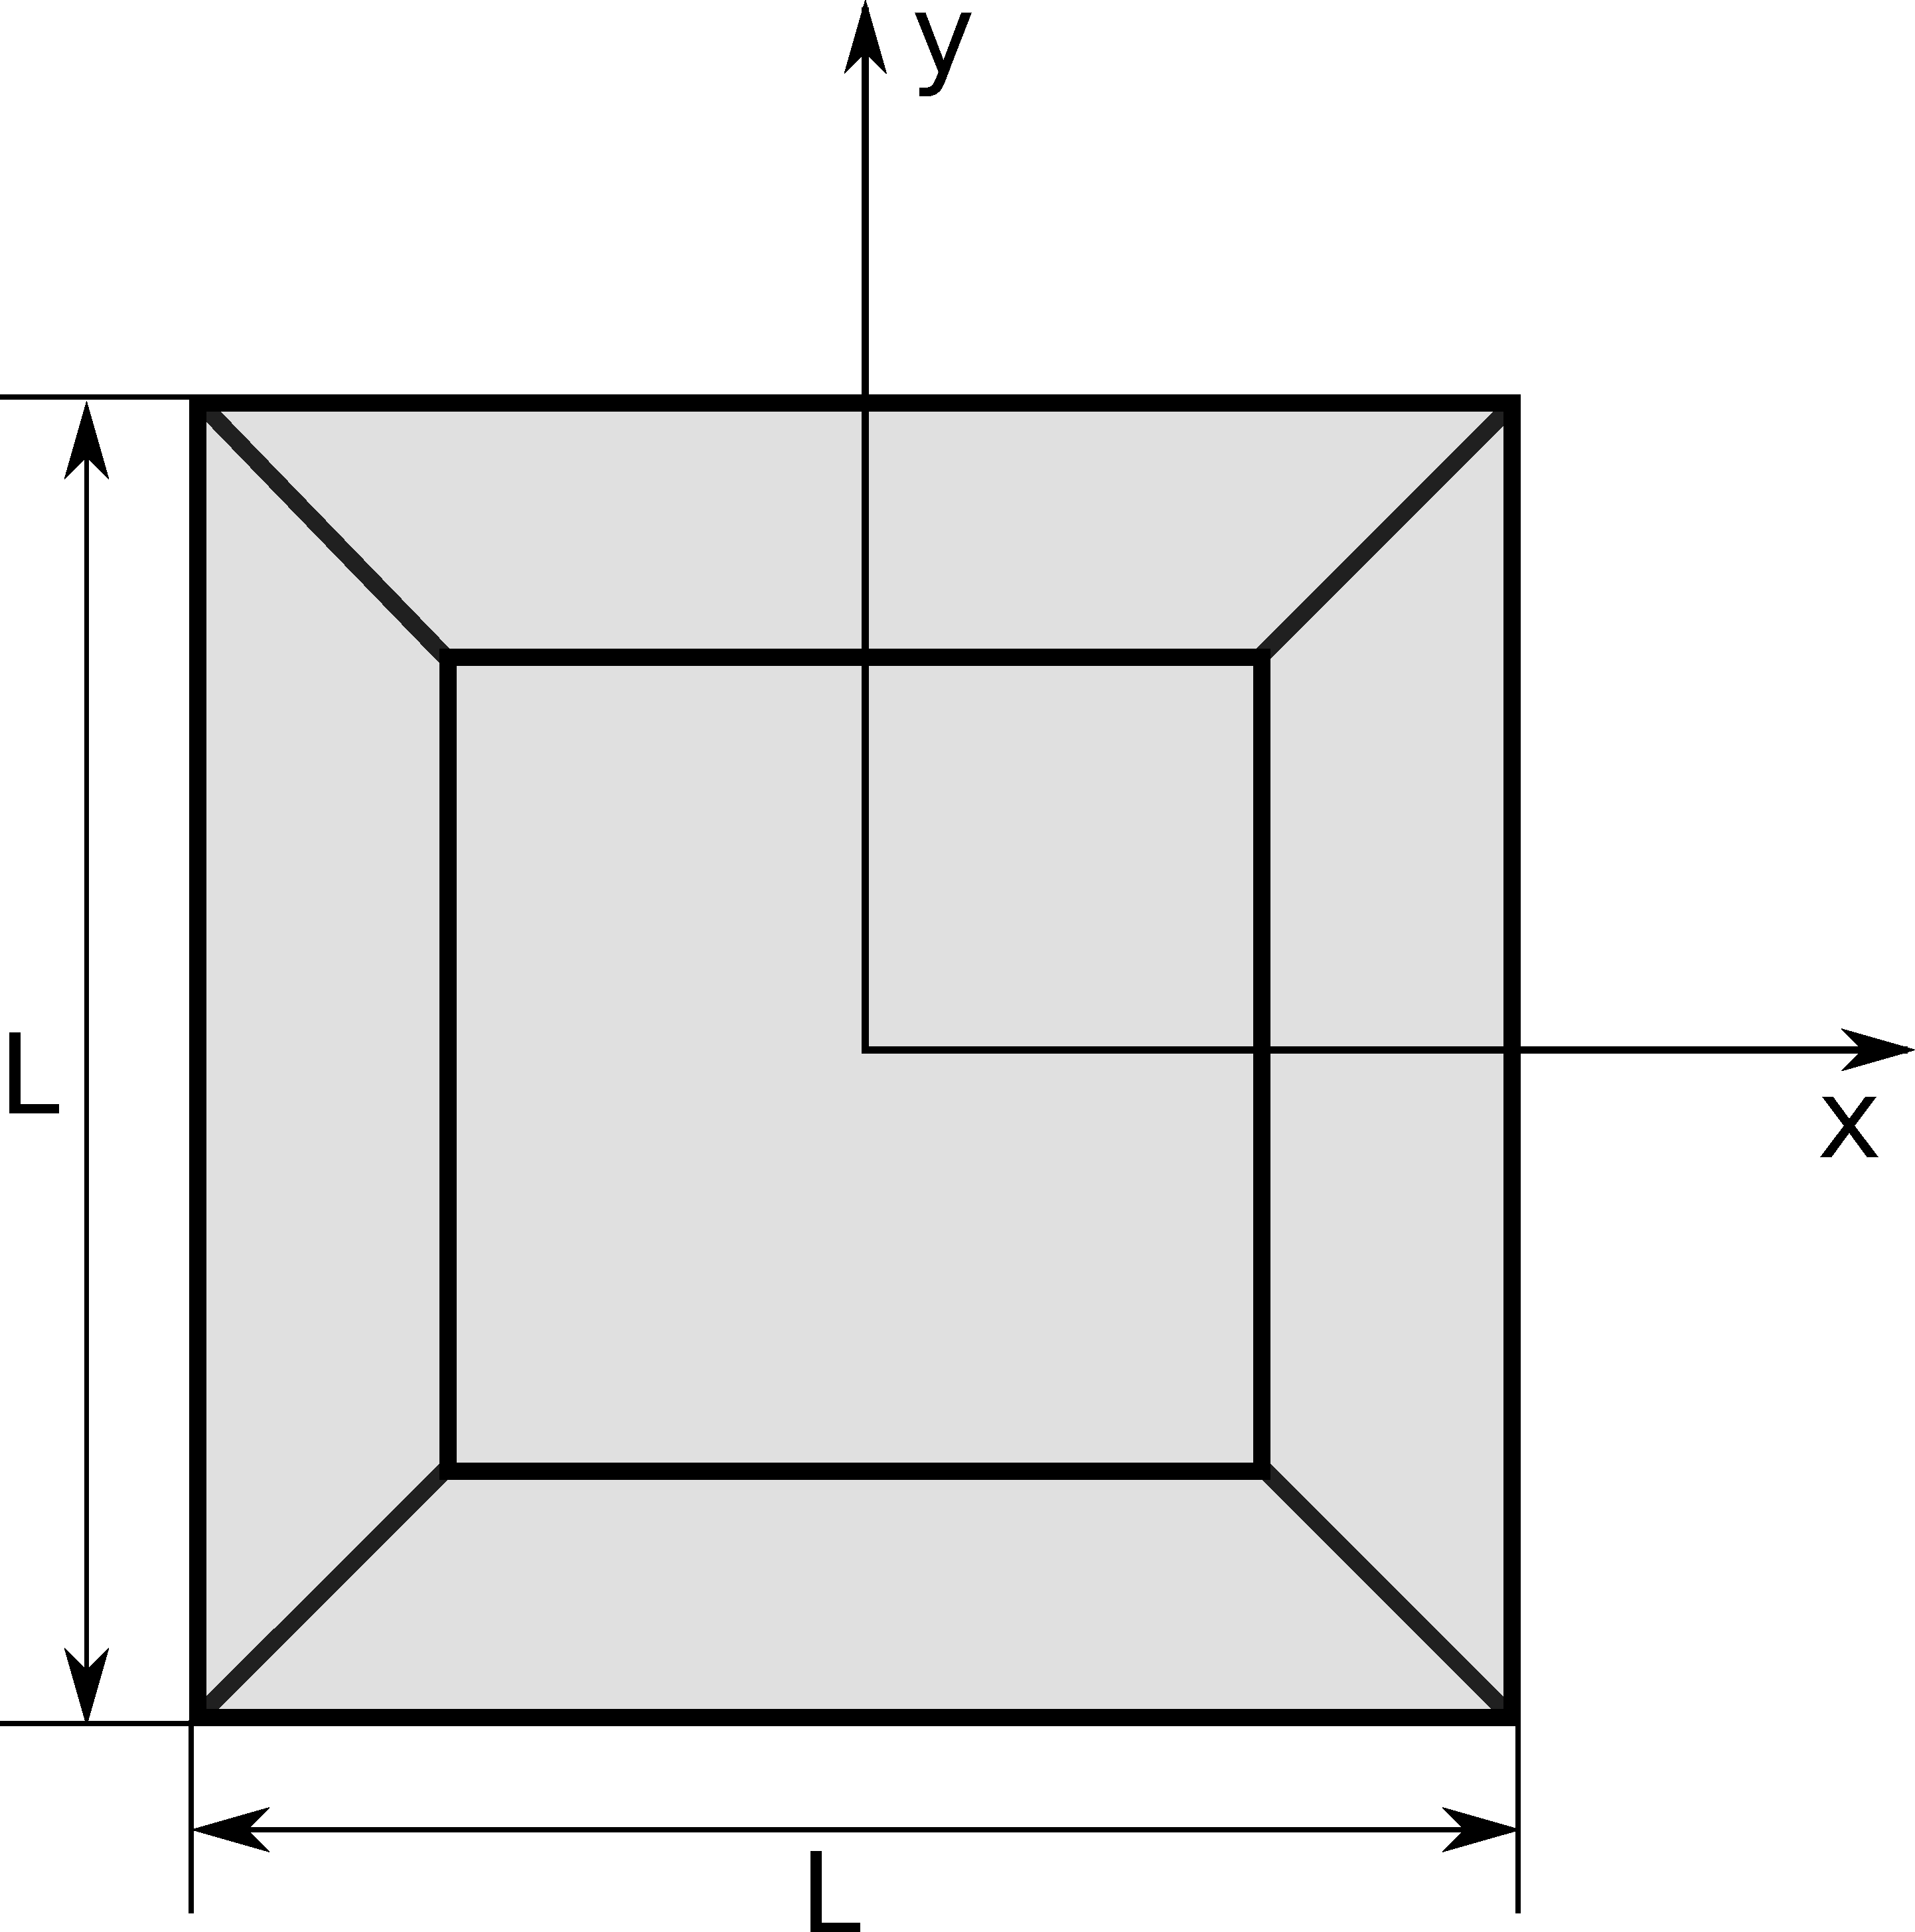
\includegraphics[width=5cm]{fig/cuts/Cuboctahedron2dxy.pdf}}
\hfill
\caption{Sketch of a Cuboctahedron.}
\label{fig:cuboctahedron}
\end{figure}

\FloatBarrier

\paragraph{Parameters}
\begin{itemize}
\item length of the shared square base $L$,
\item height $H$,
\item height\_ratio $r_H$,
\item $\alpha$ is the angle between the base and the
  side faces, taken in the middle of the base lines (see
  fig.~\ref{fig:pyramid} in Sect.~\ref{sec:Pyramid}).
\end{itemize}

\paragraph{Restrictions on the parameters:} $\dfrac{2H}{L}< \tan(\alpha)$ and $\dfrac{2r_HH}{L}< \tan(\alpha)$.

\paragraph{Properties}
\begin{itemize}
\item volume $ V= \dfrac{1}{6} \tan(\alpha)L^3 \Big[ 2
         - \Big(1 - \dfrac{2H }{L\tan(\alpha)} \Big)^3
           - \Big(1 - \dfrac{2 r_H
             H}{L\tan(\alpha) }\Big)^3\Big]$,
\item particle surface seen from above $S =L^2$.
\end{itemize}

\paragraph{Form factor}
\begin{equation*}
F(\mathbf{q}, L, H, r_H, \alpha)=\exp(iq_z
H)\Big[F_{\rm{Pyramid}}(q_x,q_y, q_z, L, r_H H,
\alpha)+F_{\rm{Pyramid}}(q_x, q_y, -q_z, L, H, \alpha))\Big]
\end{equation*}

\paragraph{Syntax}\strut\\
\Code{FormFactorCuboctahedron(length, height, height\_ratio, alpha)}

\paragraph{Example}\strut\\
Figure~\ref{fig:FFcuboctahEx} shows the normalized intensity $|F|^2/V^2$, computed with $L=20$~nm, $H=13$~nm, $r_H=0.7$, and $\alpha=60^{\circ}$.
\begin{figure}[ht]
\begin{center}
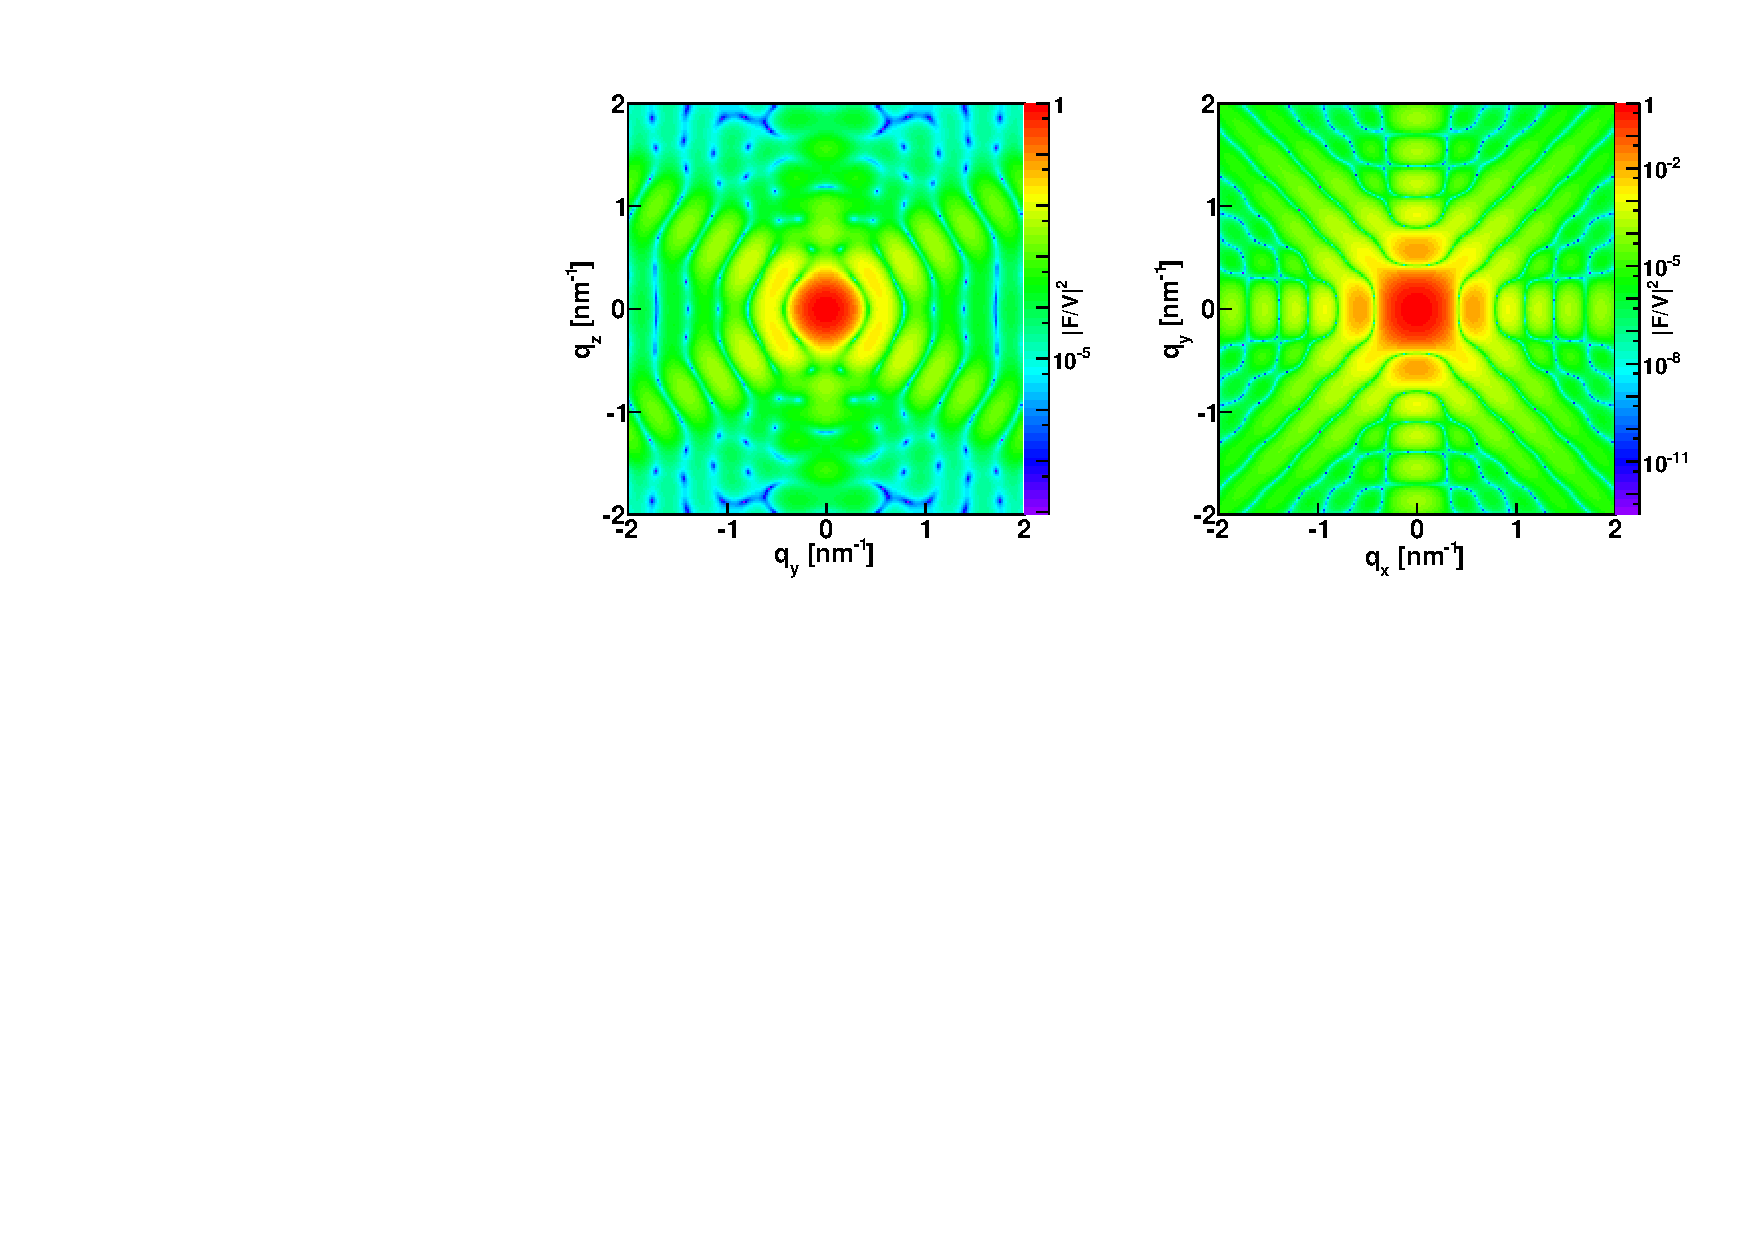
\includegraphics[angle=-90,width=\textwidth]{fig/ff/figffcuboctah.pdf}
\end{center}
\caption{Normalized intensity for the form factor of a cuboctahedron plotted against ($q_y$, $q_z$) and  ($q_x$, $q_y$) and computed with \Code{FormFactorCuboctahedron(20.*nanometer, 13.*nanometer, 0.7, 60.*degree)}.}
\label{fig:FFcuboctahEx}
\end{figure}

\paragraph{References}\strut\\
Agrees with \lq\lq Cuboctahedron\rq\rq\ form factor of \IsGISAXS~\cite{Laz02},
except for different parametrization $L=2R_{\rm{\Code{IsGISAXS}}}$.

%-------------------------------------------------------------------------------
\newpage
\subsection{Cylinder} \label{sec:Cylinder}
  \index{Cylinder (form factor)}
  \index{FormFactorCylinder@\Code{FormFactorCylinder}}
%-------------------------------------------------------------------------------
 
\paragraph{Real-space geometry}\strut\\
A right circular cylinder (see fig.~\ref{fig:cylinder}).

\begin{figure}[ht]
\hfill
\subfigure[Side view]{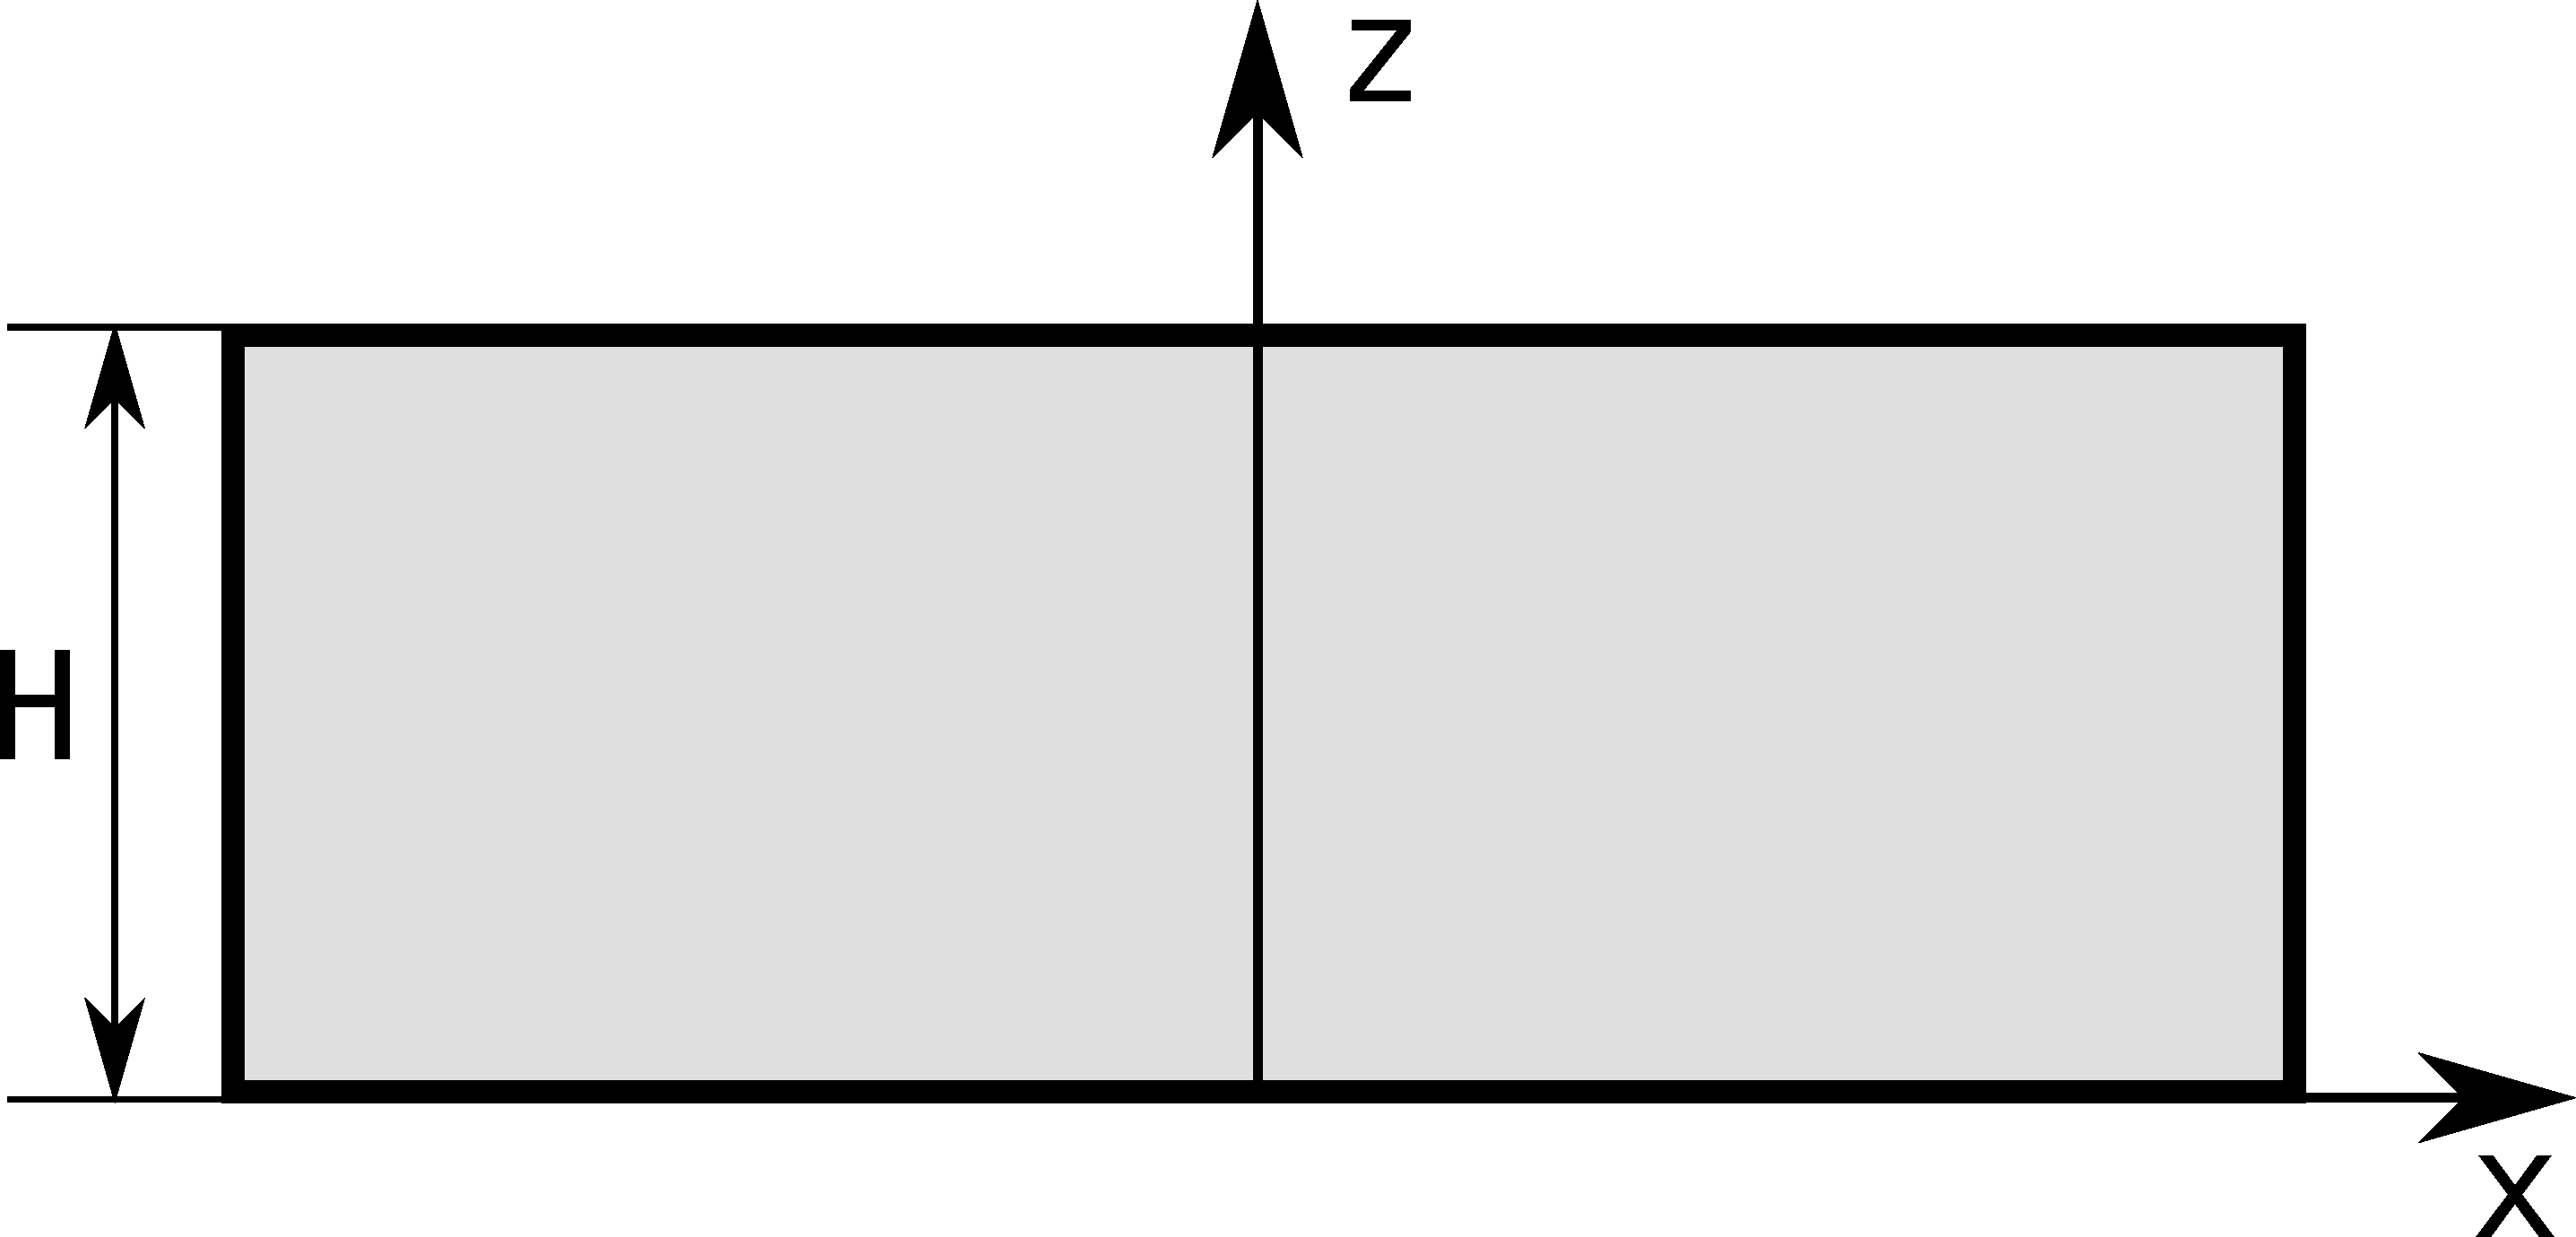
\includegraphics[width=5cm]{fig/cuts/Cylinder2dxz.pdf}}
\hfill
\subfigure[Top view]{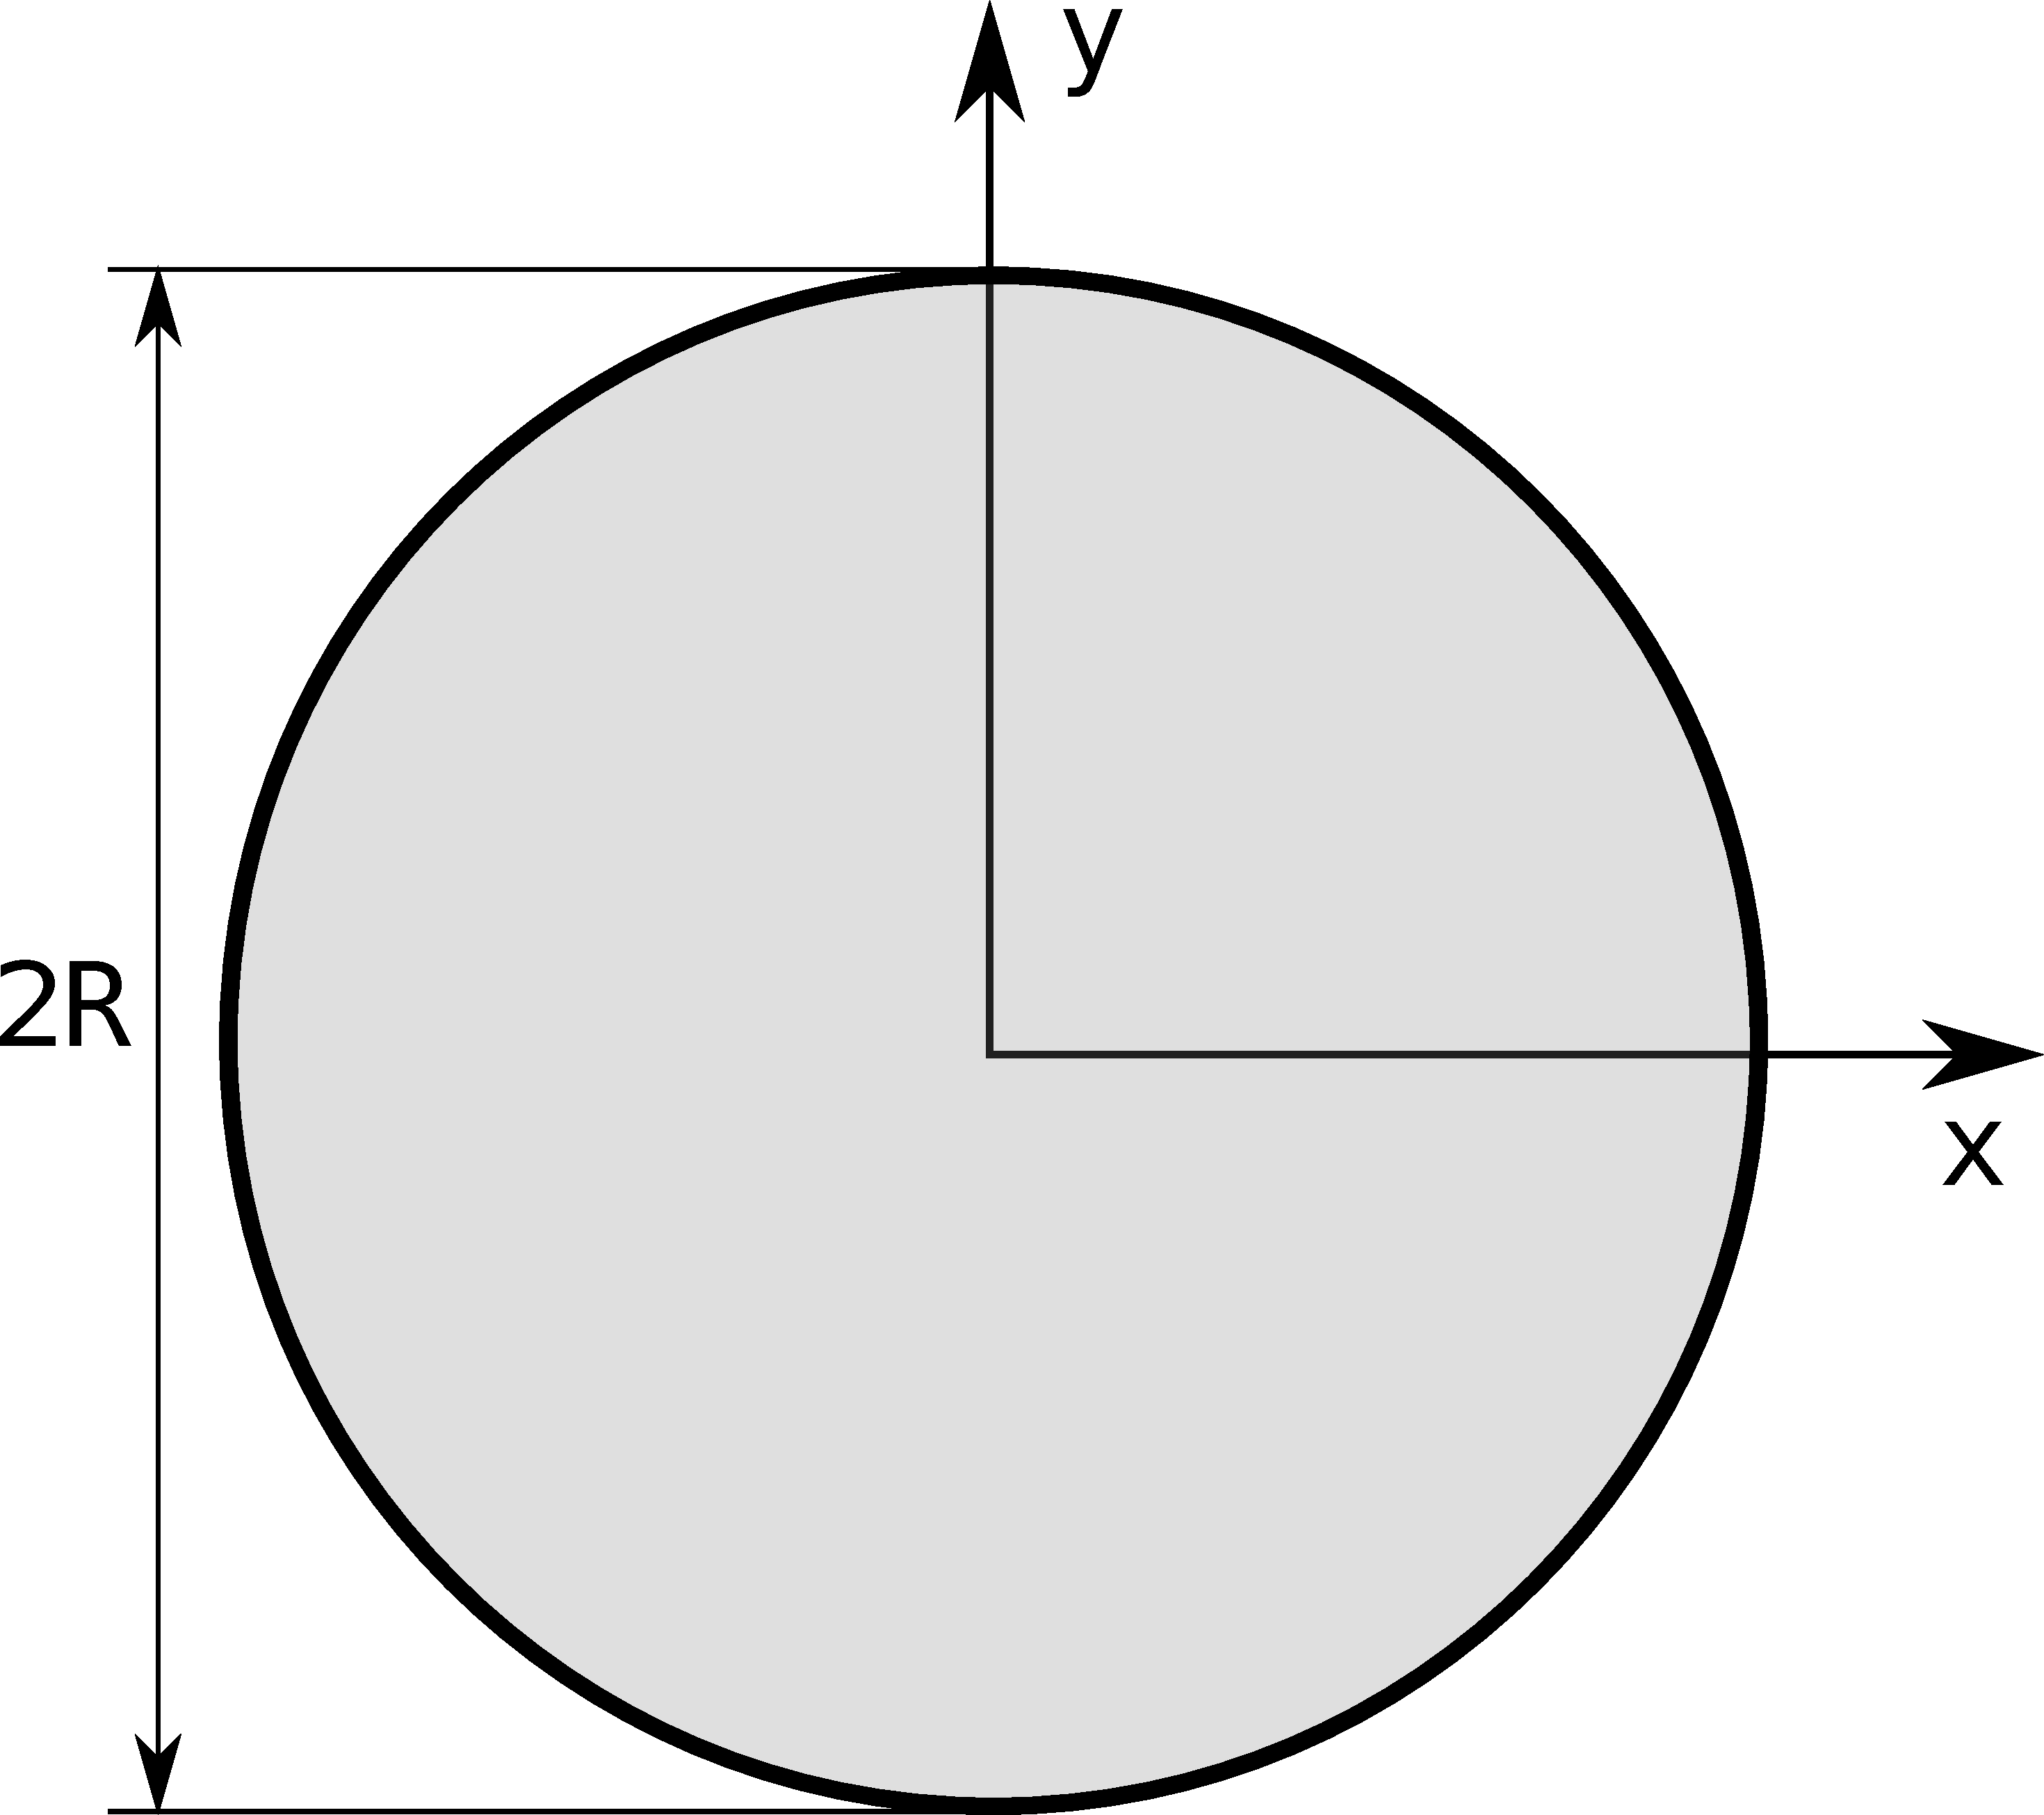
\includegraphics[width=5cm]{fig/cuts/Cylinder2dxy.pdf}}
\hfill
\caption{Sketch of a Cylinder.}
\label{fig:cylinder}
\end{figure}

\paragraph{Parameters}
\begin{itemize}
\item radius of the circular base $R$, 
\item height $H$.
\end{itemize}

\paragraph{Properties}
\begin{itemize}
\item volume $V = \pi R^2 H$,
\item particle surface seen from above $S=\pi R^2$.

\end{itemize}

\paragraph{Form factor}
  \begin{equation*}
F(\mathbf{q},R, H)=  2\pi
 R^2 H  \sinc\left(q_ z \frac{H}{2}\right) \exp\left(i q_ z \frac{H}{2}\right) \frac{J_1(q_{\parallel} R )}{q_{\parallel} R },
 \end{equation*}
with $q_{\parallel}=\sqrt{q_x^2+q_y^2}$ and $J_1(x)$ is the first order
Bessel function of the first kind \cite{AbSt64}.

\paragraph{Syntax}\strut\\
\Code{FormFactorCylinder(radius, height)}

\newpage

\paragraph{Example}\strut\\
Figure~\ref{fig:FFcylinderEx} shows the normalized intensity
$|F|^2/V^2$, computed with $R=8$~nm and \mbox{$H=16$~nm.}
\begin{figure}[ht]
\begin{center}
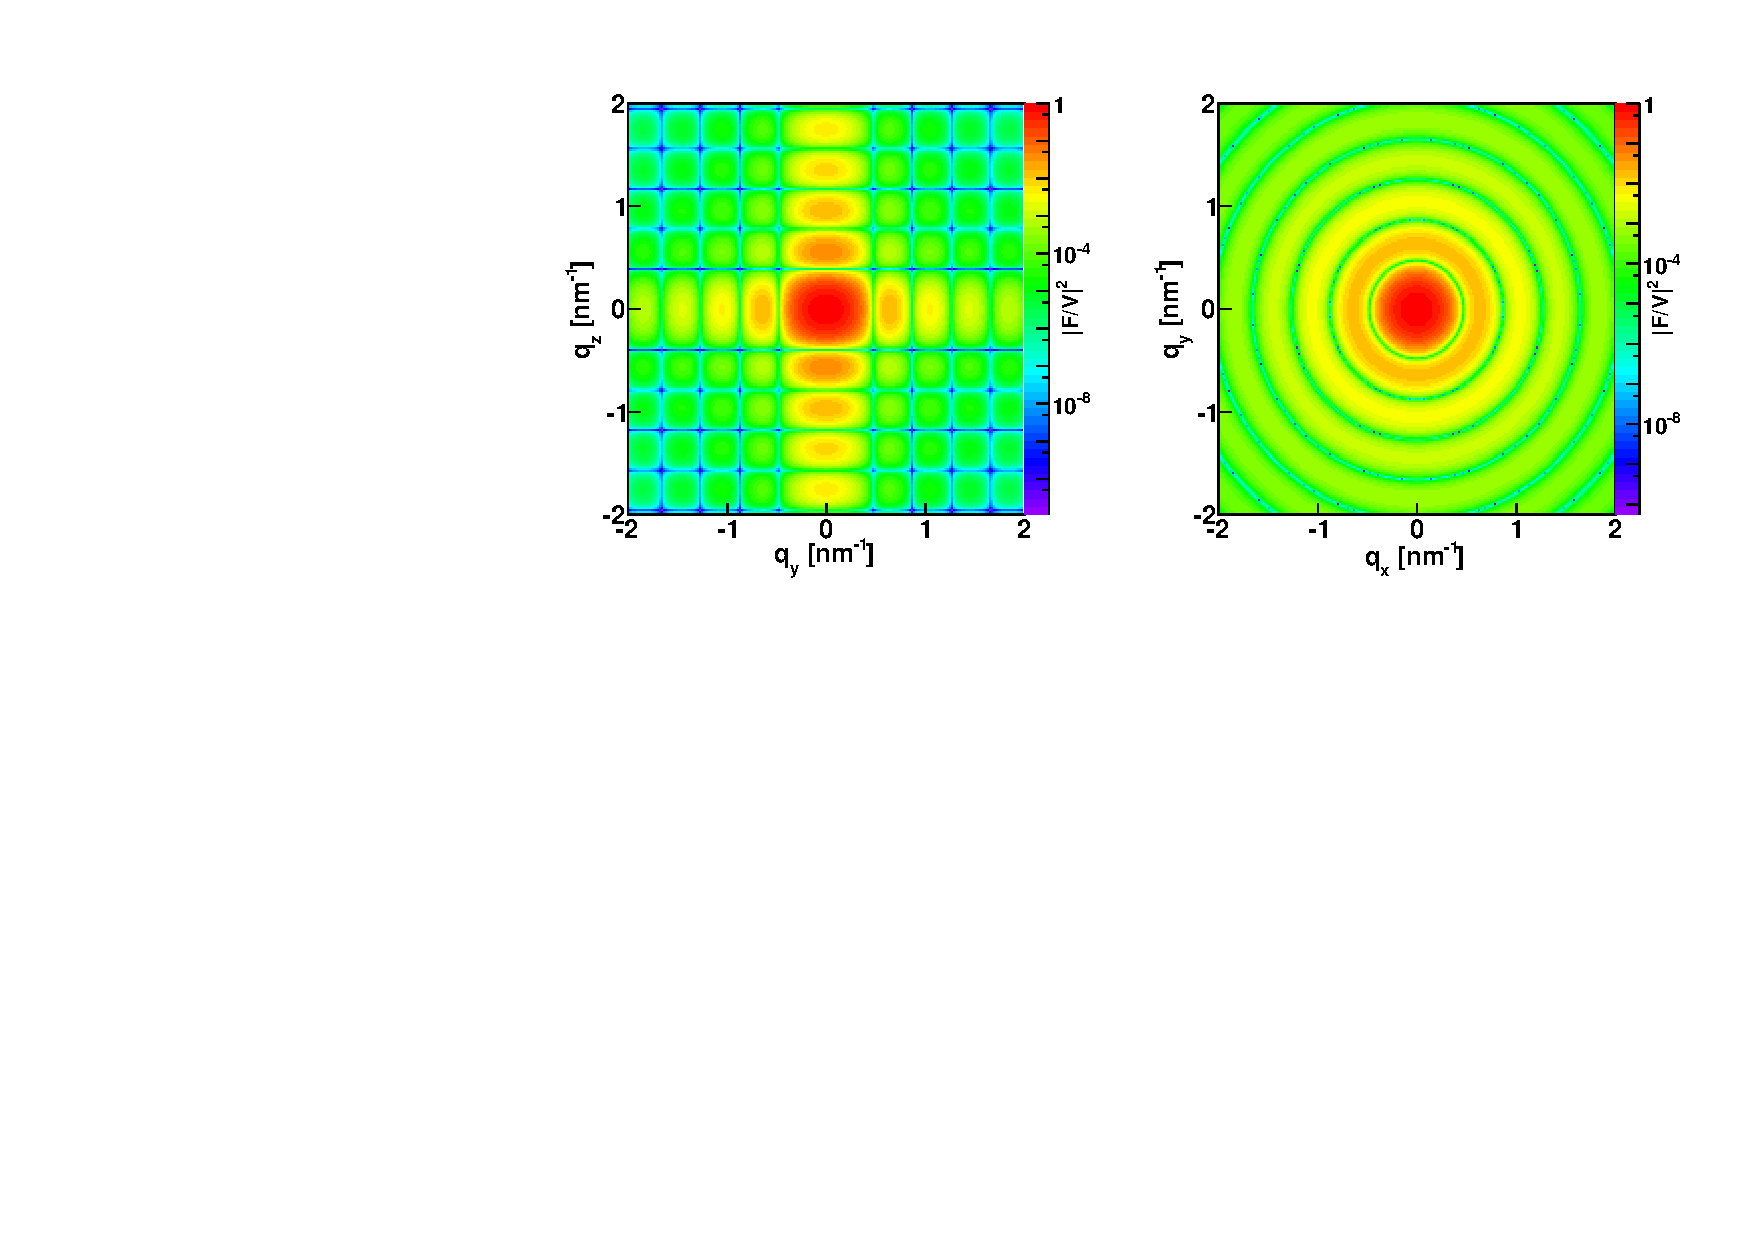
\includegraphics[angle=-90,width=\textwidth]{fig/ff/figffcylinder.pdf}
\end{center}
\caption{Normalized intensity for the form factor of a cylinder plotted against ($q_y$, $q_z$) and  ($q_x$, $q_y$.) It
has been  computed with \Code{FormFactorCylinder(8.*nanometer, 16.*nanometer)}.}
\label{fig:FFcylinderEx}
\end{figure}

\paragraph{References}\strut\\
Agrees with \lq\lq Cylinder\rq\rq\ form factor of \IsGISAXS~\cite{Laz02}.

%-------------------------------------------------------------------------------
\newpage
\subsection{EllipsoidalCylinder} \label{sec:EllipsoidalCylinder} 
  \index{Ellipsoidal cylinder (form factor)}
  \index{Cylinder (form factor)!ellipsoidal}
  \index{FormFactorEllipsoidalCylinder@\Code{FormFactorEllipsoidalCylinder}}
%-------------------------------------------------------------------------------

\paragraph{Real-space geometry}\strut\\
A cylinder whose cross section is an ellipse.

\begin{figure}[ht]
\hfill
\subfigure[Side view]{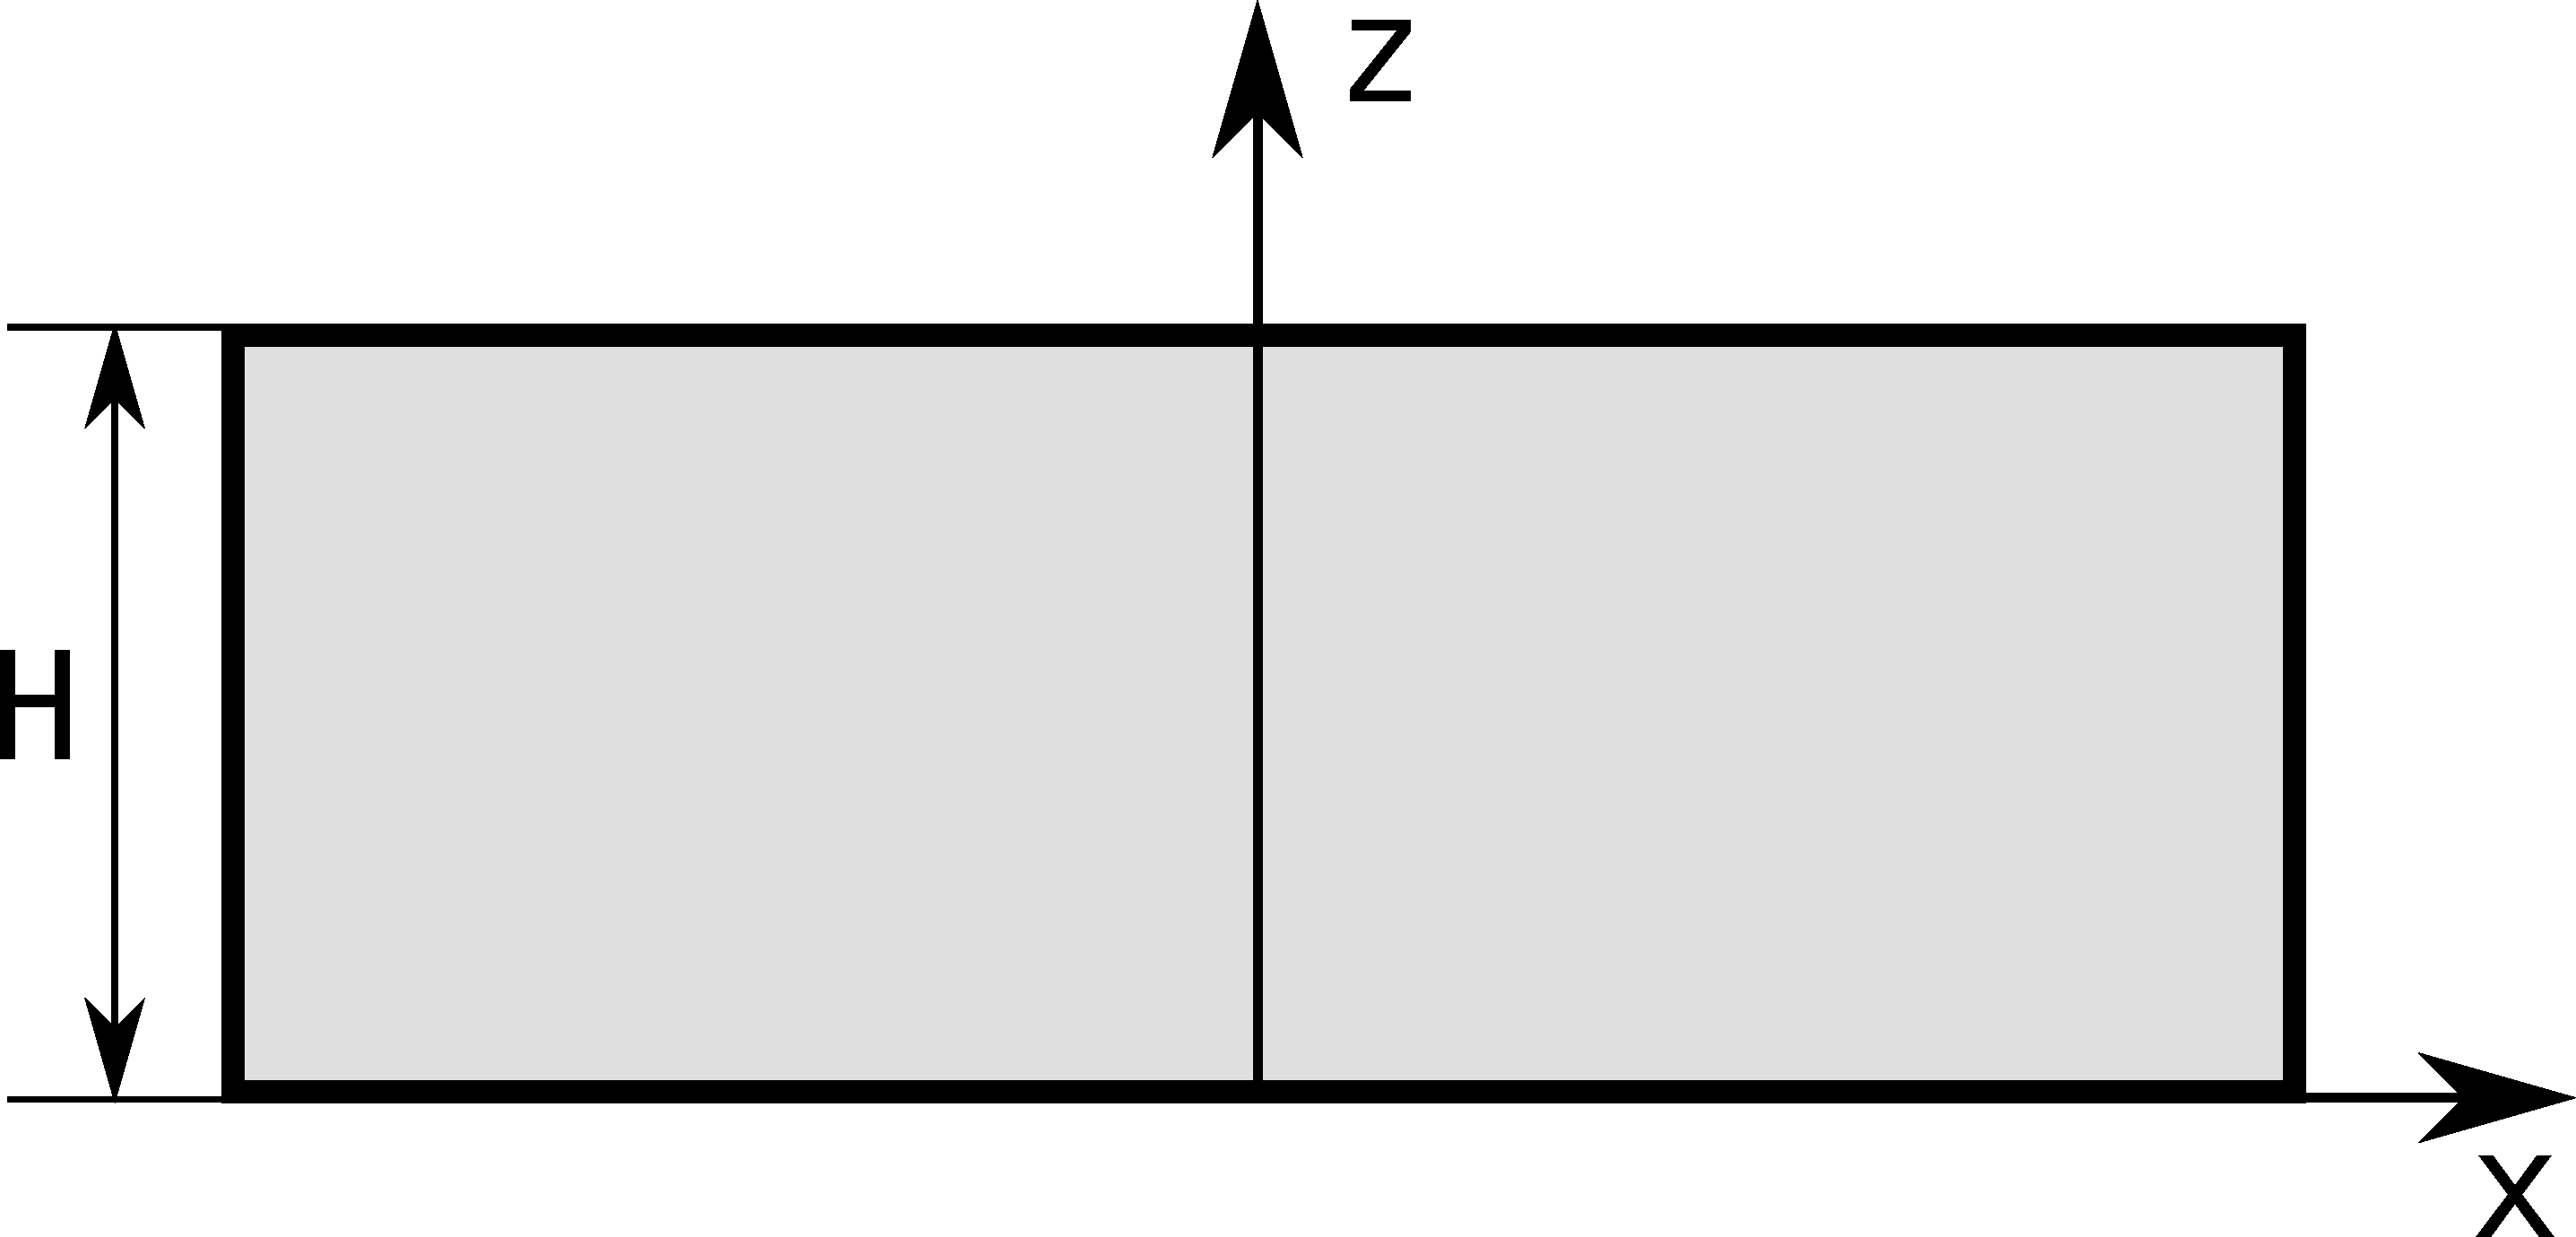
\includegraphics[width=5cm]{fig/cuts/EllipsoidalCylinder2dxz.pdf}}
\hfill
\subfigure[Top view]{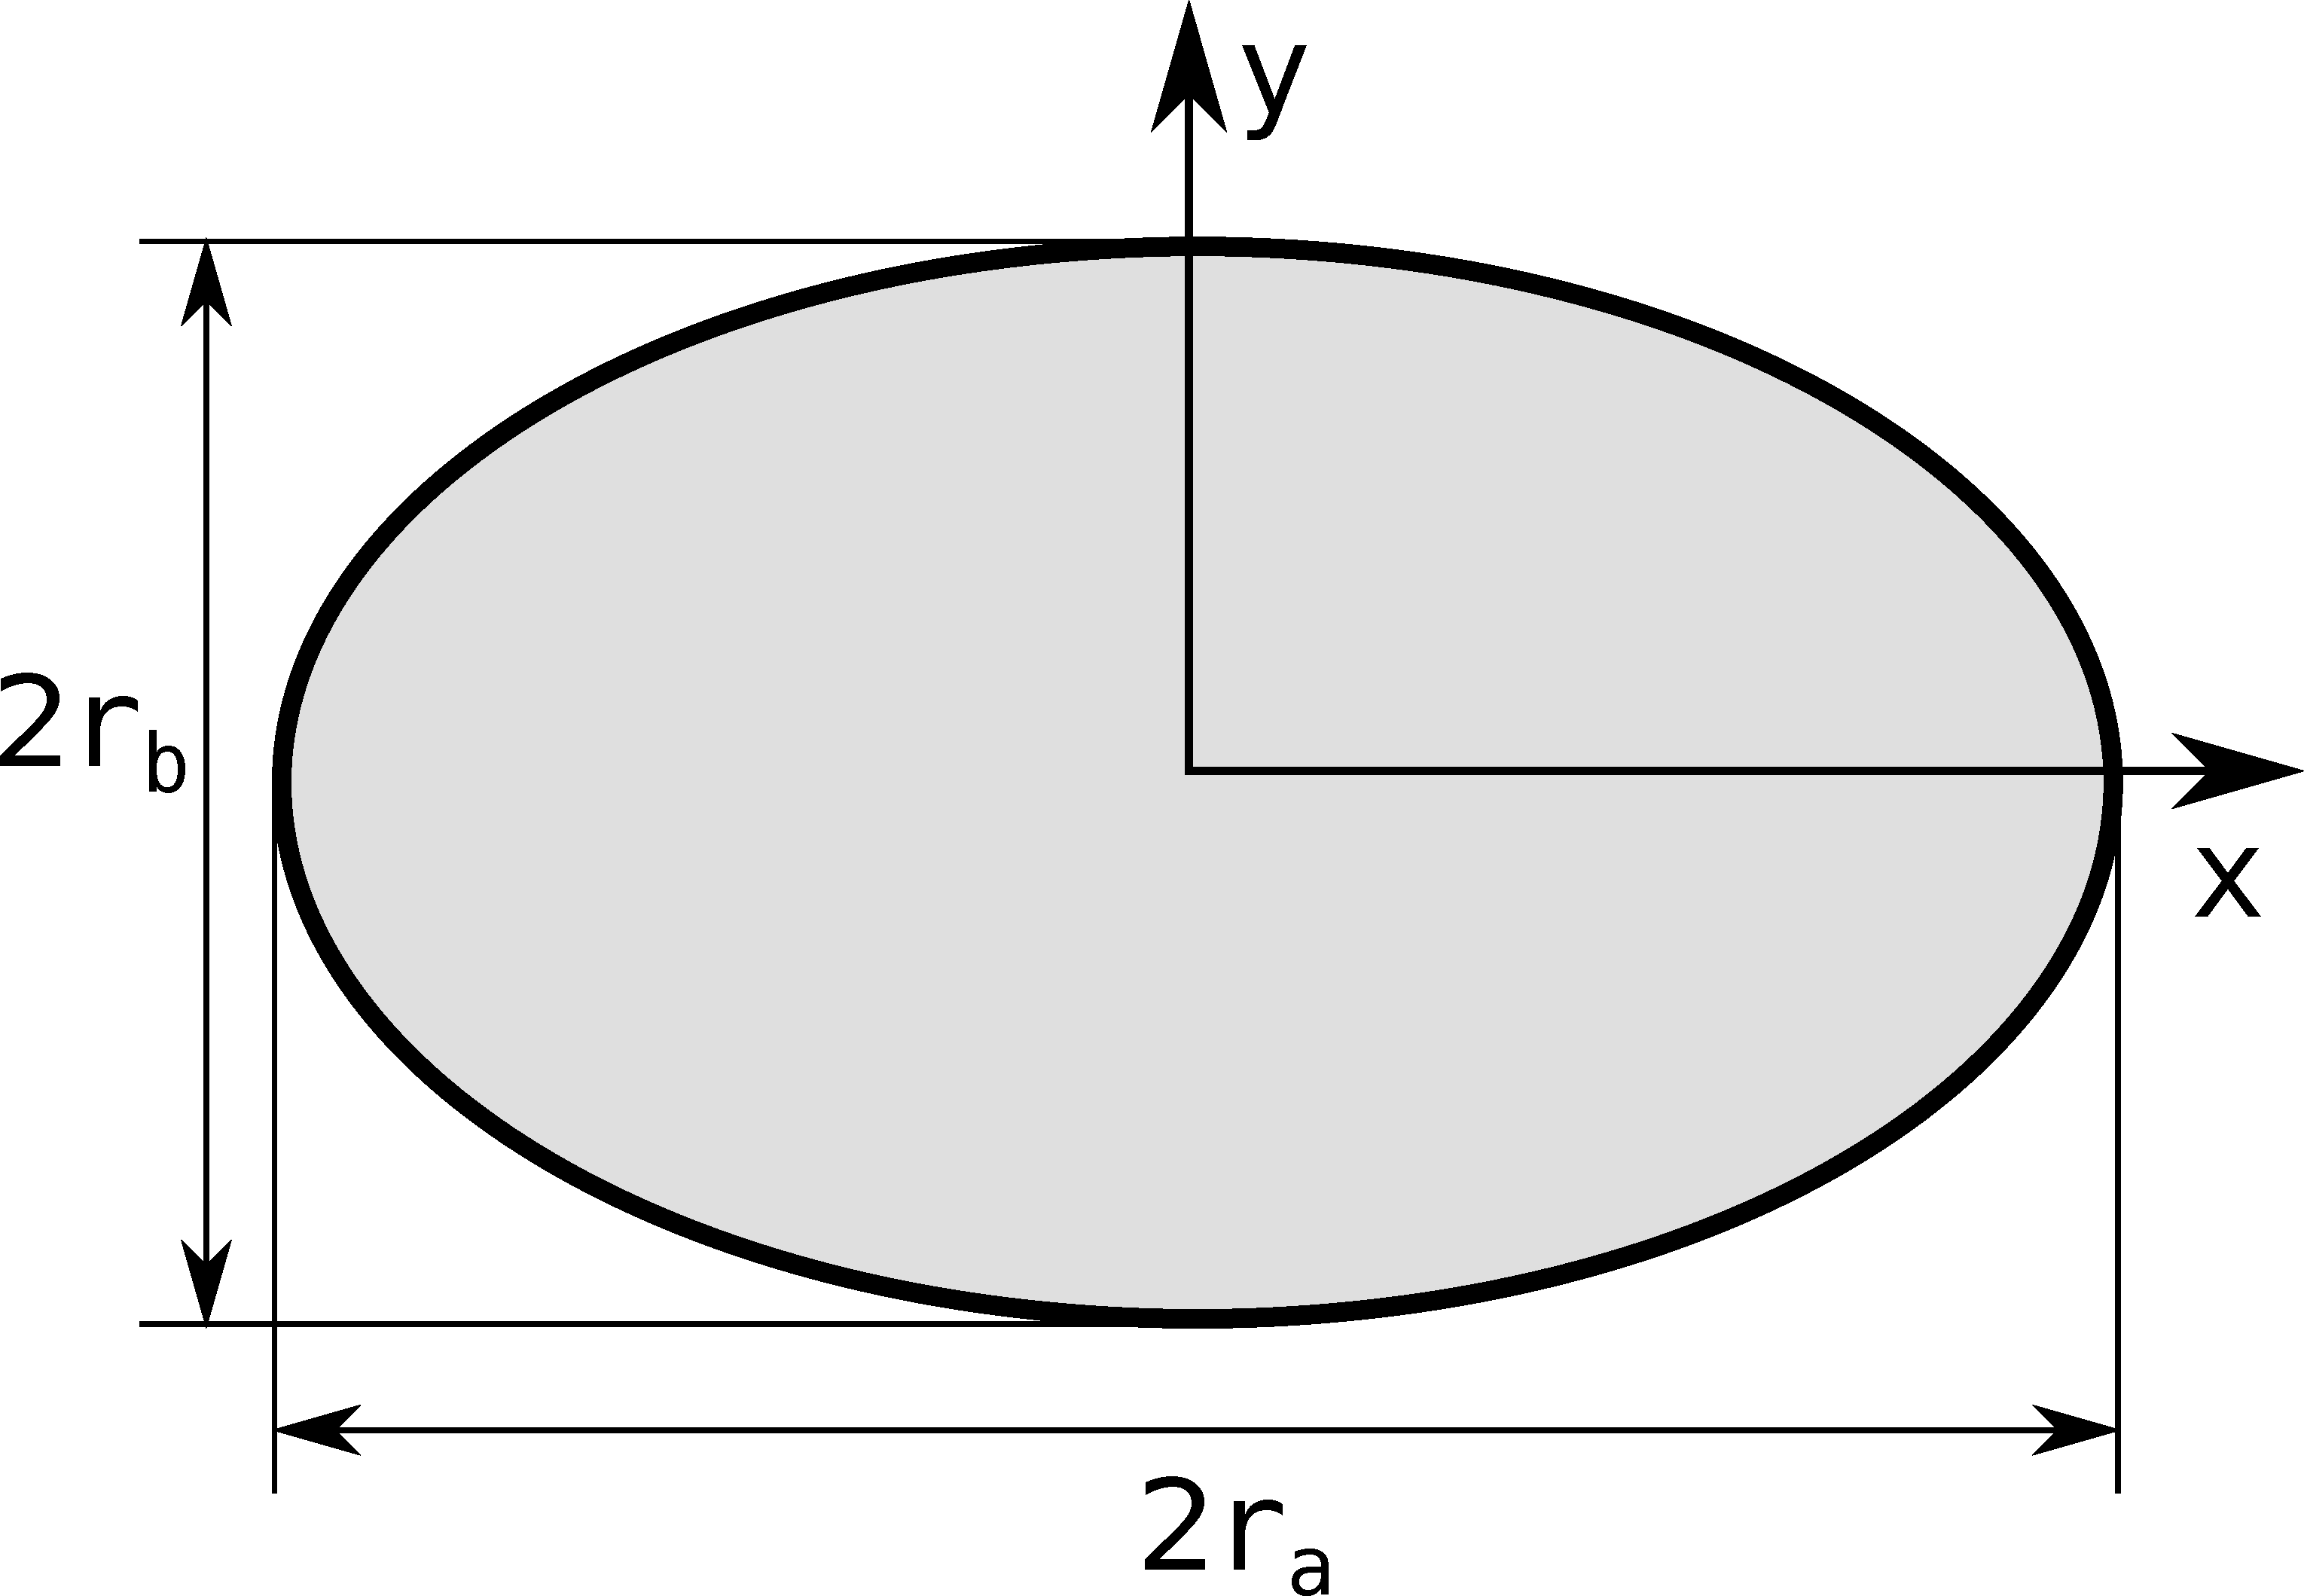
\includegraphics[width=5cm]{fig/cuts/EllipsoidalCylinder2dxy.pdf}}
\hfill
\caption{Sketch of an Ellipsoidal Cylinder.}
\label{fig:ellipscylinder}
\end{figure}

\paragraph{Parameters}
\begin{itemize}
\item $r_a$ = half length of the ellipse main axis parallel to $x$,
\item$r_b$ = half length of the ellipse main axis parallel to $y$, 
\item height $H$.
\end{itemize}

\paragraph{Properties}
\begin{itemize}
\item volume $V = \pi r_a r_bH$,
\item particle surface seen from above $S = r_a r_b$.
\end{itemize}

\paragraph{Form factor}
The total form factor is given by 
\begin{equation*}
F(\mathbf{q},R,W,H) = 2\pi r_a r_b H \exp\left(i\frac{q_z
  H}{2}\right)\sinc\left(\frac{q_z H}{2}\right) \frac{J_1(\gamma)}{\gamma},
\end{equation*}
with $\gamma=\sqrt{(q_x r_a)^2+(q_y r_b)^2}$ and $J_1(x)$ is the first order
Bessel function of the first kind \cite{AbSt64}.

\paragraph{Syntax}\strut\\
\Code{FormFactorEllipsoidalCylinder($r_a$, $r_b$, height)}

\newpage


\paragraph{Example}\strut\\
Figure~\ref{fig:FFellipscylinderEx} shows the normalized intensity
$|F|^2/V^2$, computed with $r_a=8$~nm, $r_b=13$~nm, and $H=16$~nm.
\begin{figure}[ht]
\begin{center}
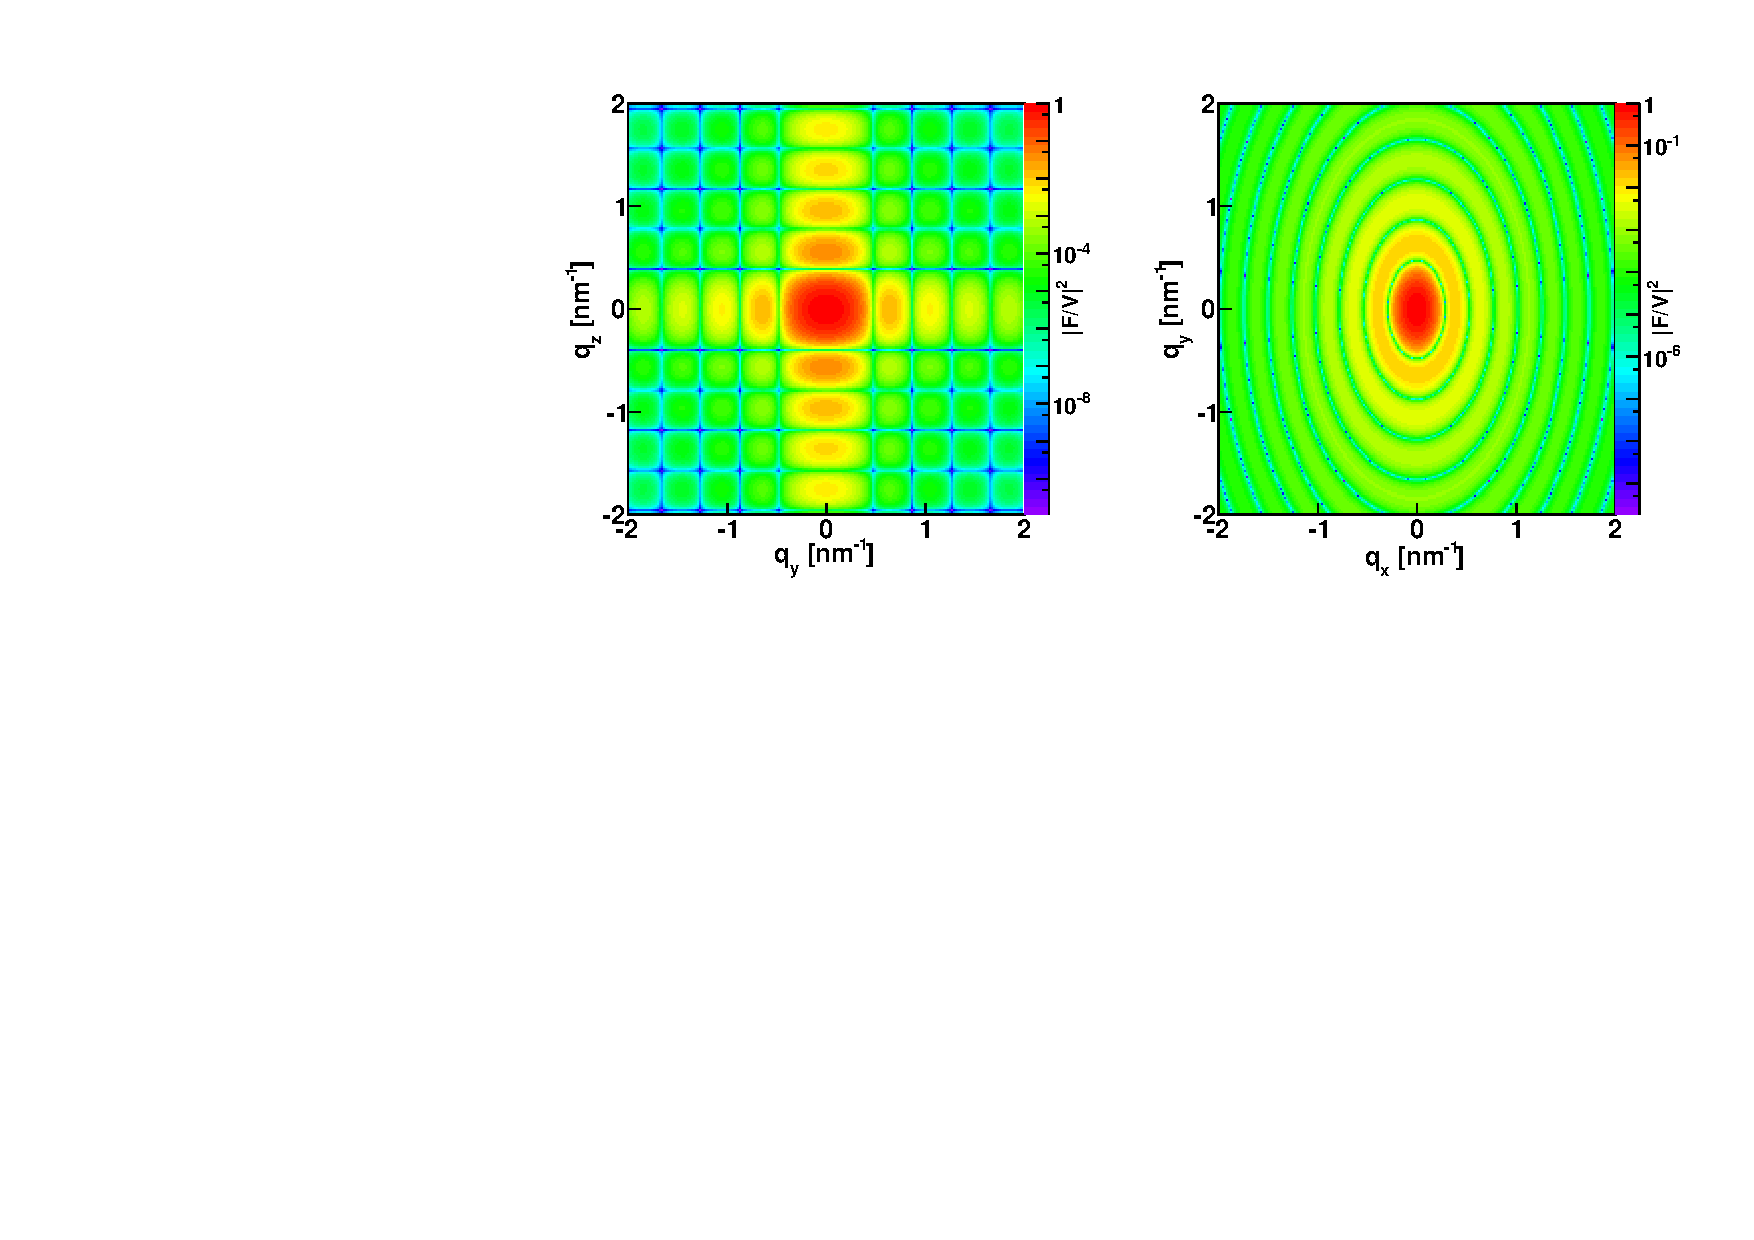
\includegraphics[angle=-90,width=\textwidth]{fig/ff/figffellipscylinder.pdf}
\end{center}
\caption{Normalized intensity for the form factor of an ellipsoidal
  cylinder plotted against ($q_y$, $q_z$) and ($q_x$,
  $q_y$) and computed with \Code{FormFactorEllipsoidalCylinder(8.*nanometer, 13.*nanometer, 16*nanometer)}.}
\label{fig:FFellipscylinderEx}
\end{figure}

\paragraph{References}\strut\\
Agrees with \lq\lq Ellipsoid\rq\rq\ form factor of \IsGISAXS~\cite{Laz02}.

%-------------------------------------------------------------------------------
\newpage
\subsection{Cone (circular)} \label{sec:Cone} 
  \index{Cone (form factor)!circular}
  \index{Truncated cone (form factor)}
  \index{FormFactorCone@\Code{FormFactorCone}}
%-------------------------------------------------------------------------------

\paragraph{Real-space geometry}
A truncated cone as shown in fig.~\ref{fig:cone}. 

\begin{figure}[ht]
\hfill
\subfigure[Side view]{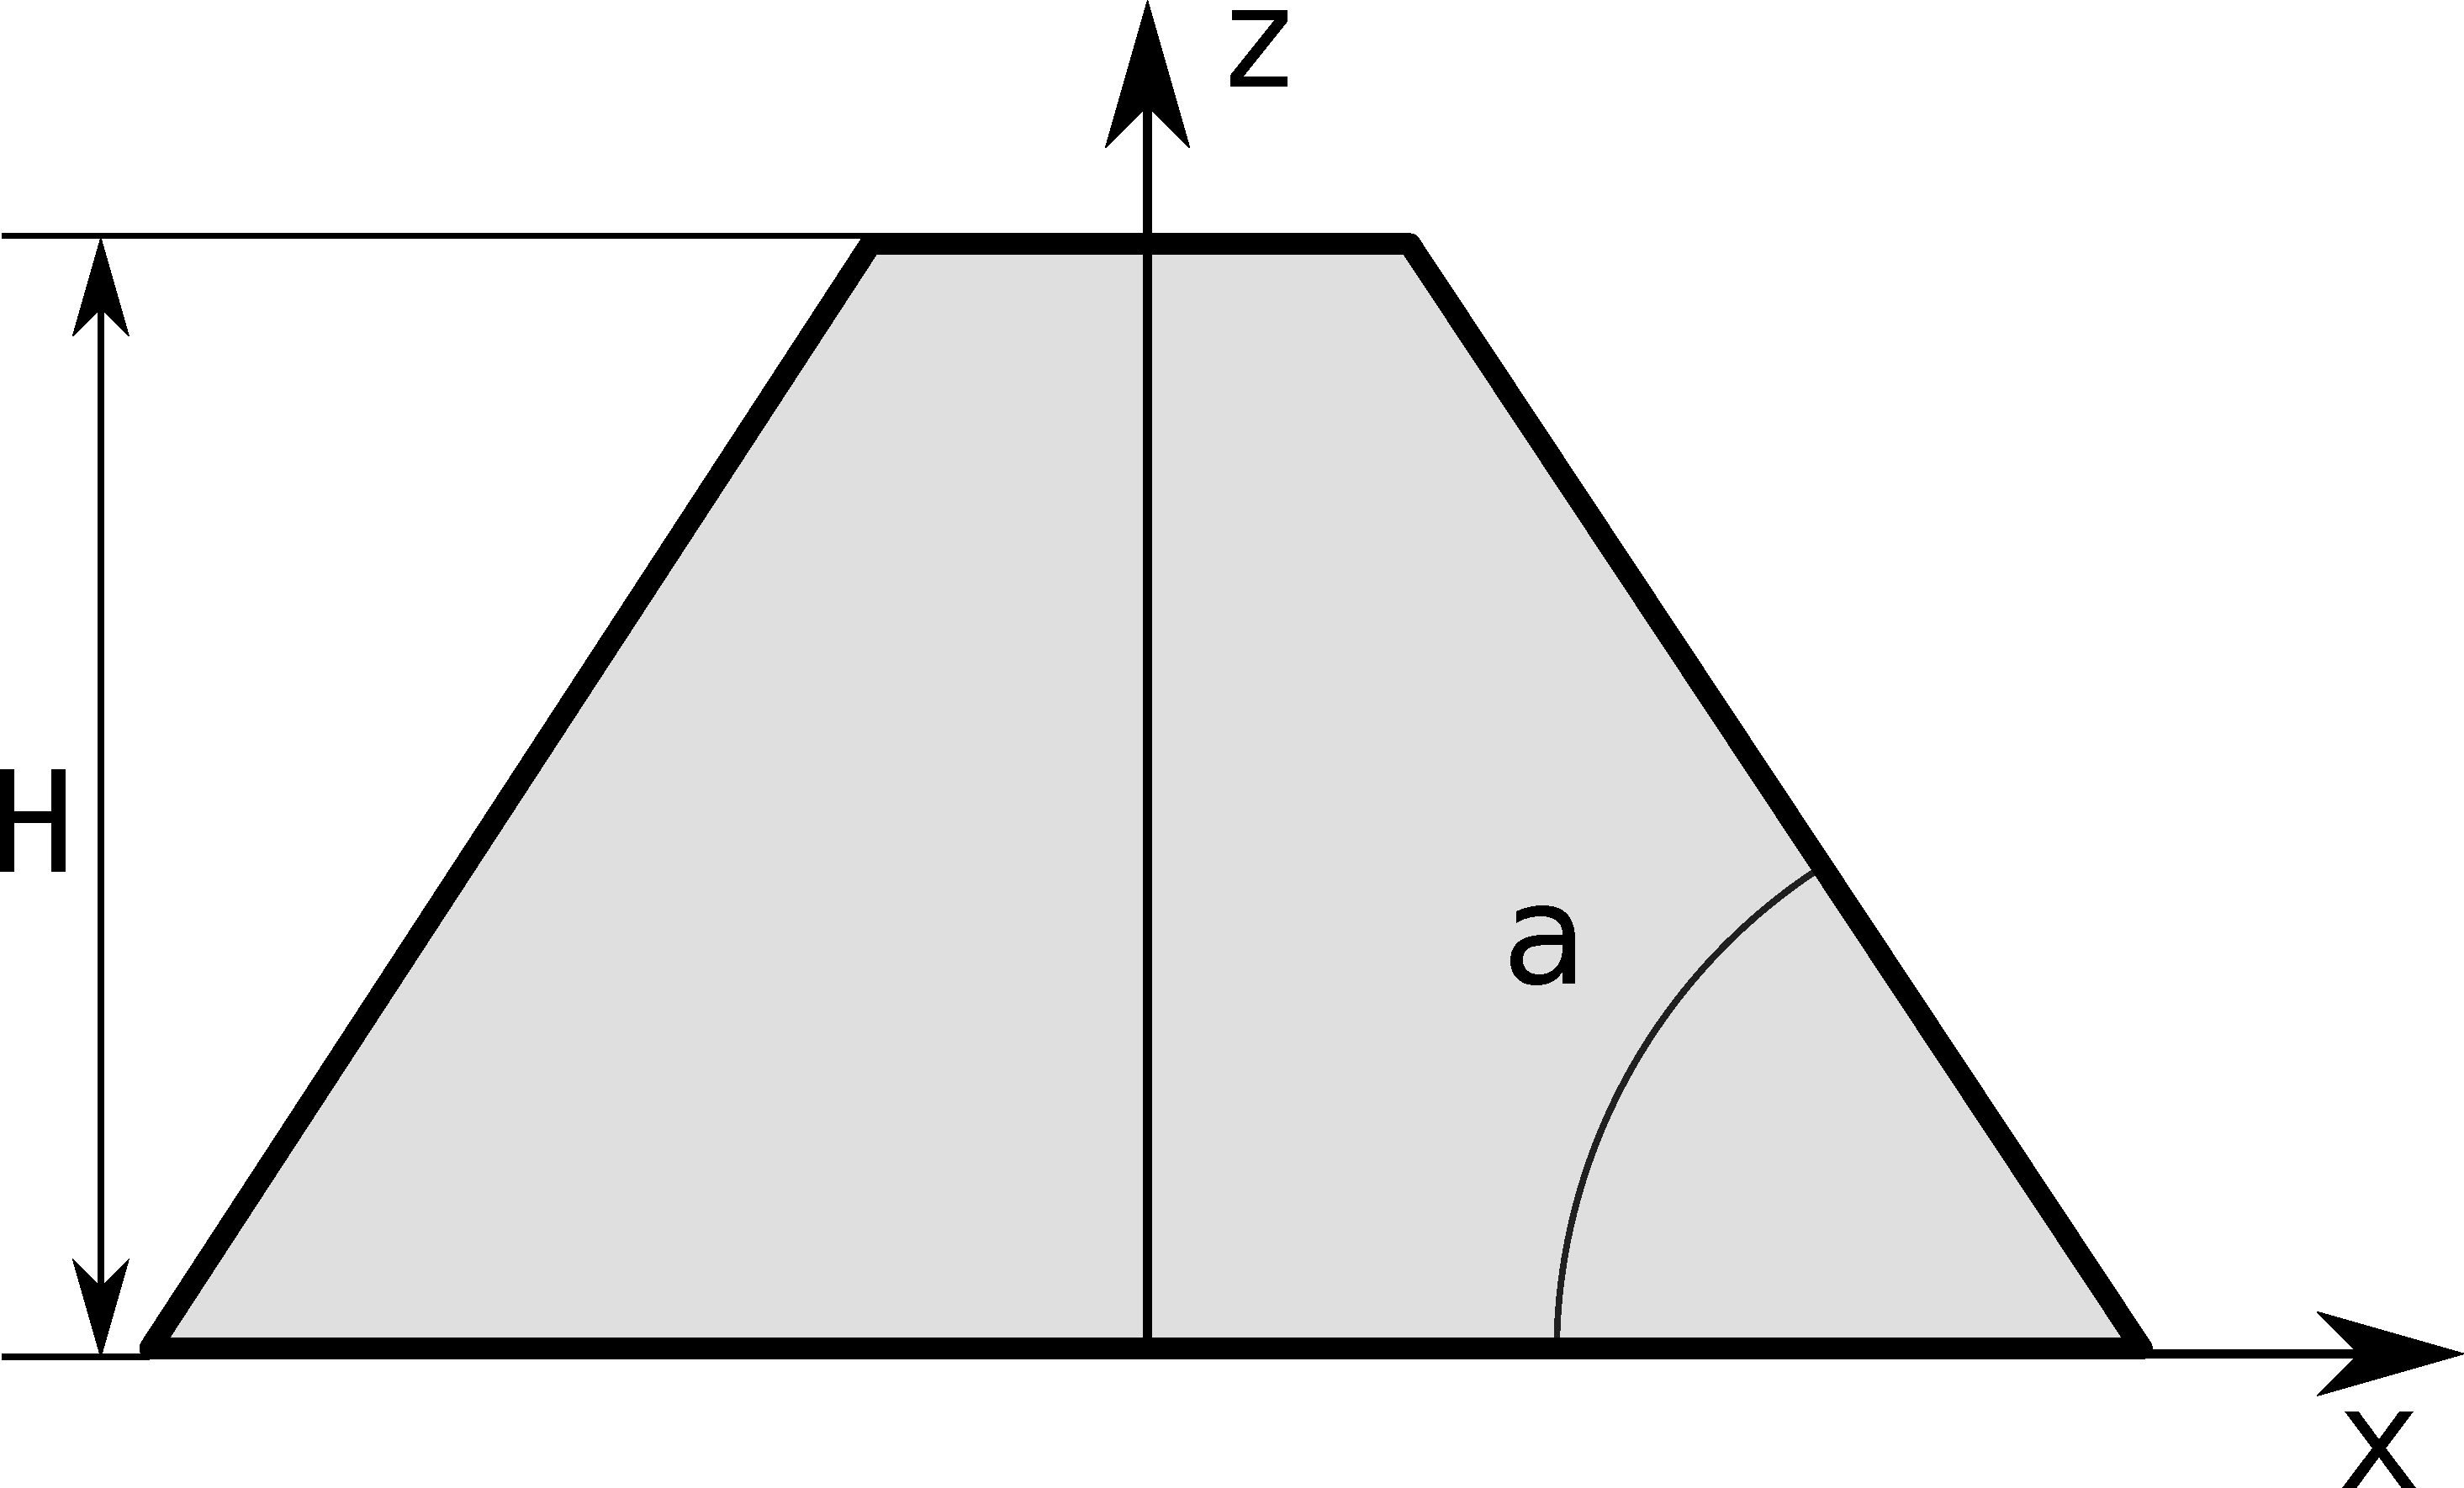
\includegraphics[width=5cm]{fig/cuts/Cone2dxz.pdf}}
\hfill
\subfigure[Top view]{\includegraphics[width=5cm]{fig/cuts/Cone2dxy.pdf}}
\hfill
\caption{Sketch of a Cone.}
\label{fig:cone}
\end{figure}

\paragraph{Parameters}
\begin{itemize}
\item radius $R$,
\item height $H$,
\item $\alpha$ is the angle between the side and the circular base.
\end{itemize}

\paragraph{Restrictions on the parameters:} $\dfrac{H}{R}< \tan(\alpha)$.

\paragraph{Properties}
\begin{itemize}
\item volume $V = \dfrac{\pi}{3} \tan(\alpha) R^3 \left[ 
            1 - \left(1- \dfrac{H}{\tan(\alpha)R}\right)^3\right]$,
\item  particle surface seen from above $S=\pi R^2$.
\end{itemize}

\paragraph{Form factor}
\begin{equation*}
F(\mathbf{q}, R, H, \alpha) = \int_0 ^H 2\pi R_z^2
\frac{J_1(q_{\parallel}R_z)}{q_{\parallel} R_z}\exp(iq_z z)dz,
\end{equation*}
with $R_z =R-\dfrac{z}{\tan \alpha}$, $\mathbf{q}_{\parallel}=\sqrt{q_x^2+ q_y^2}$ and $J_1(x)$ is the first order
Bessel function of the first kind \cite{AbSt64}.

\paragraph{Syntax}\strut\\
\Code{FormFactorCone(radius, height, alpha)}. 

\paragraph{Example}\strut\\
Figure~\ref{fig:FFConeEx} shows the normalized intensity
$|F|^2/V^2$, computed with $R=10$~nm, $H=13$~nm, and $\alpha=60^{\circ}$.
\begin{figure}[ht]
\begin{center}
\includegraphics[angle=-90,width=\textwidth]{fig/ff/figffcone.pdf}
\end{center}
\caption{Normalized intensity for the form factor of a Cone plotted against ($q_y$, $q_z$) and ($q_x$, $q_y$.) It
  has been  computed with \Code{FormFactorCone(10.*nanometer,13.*nanometer, 60.*degree)}.}
\label{fig:FFConeEx}
\end{figure}

\paragraph{References}\strut\\
Agrees with \lq\lq Cone\rq\rq\ form factor of \IsGISAXS~\cite{Laz02}.

%-------------------------------------------------------------------------------
\newpage
\subsection{FullSphere} \label{sec:FullSphere}
  \index{Full sphere (form factor)}
  \index{Sphere (form factor)}
  \index{FormFactorFullSphere@\Code{FormFactorFullSphere}}
%-------------------------------------------------------------------------------

\paragraph{Real-space geometry}\strut\\
The full sphere is parametrized by its radius $R$. 

\begin{figure}[ht]
\hfill
\subfigure[Side view]{\includegraphics[width=5cm]{fig/cuts/FullSphere2dxz.pdf}}
\hfill
\subfigure[Top view]{\includegraphics[width=5cm]{fig/cuts/FullSphere2dxy.pdf}}
\hfill
\caption{Sketch of a Full Sphere.}
\label{fig:fullsphere}
\end{figure}

\FloatBarrier

\paragraph{Parameters} radius $R$.

\paragraph{Properties}
\begin{itemize}
\item volume $V = \dfrac{4\pi}{3}R^3$,
\item particle surface seen from above $S= \pi R^2$.
%\item radius of gyration
\end{itemize}

\paragraph{Form factor}
\begin{equation*}
F(\mathbf{q},R) = 4\pi R^3 \exp(iq_z R)\frac{\sin(q R) - q R \cos(q R)}{(qR)^3},
\end{equation*}
where $q=\sqrt{q_x^2 + q_y^2 + q_z^2}$.

\paragraph{Syntax}\strut\\
\Code{FormFactorFullSphere(radius)}

\newpage

\paragraph{Example}\strut\\
Figure~\ref{fig:FFfSphereEx} shows the normalized intensity $|F|^2/V^2$, computed with $R=8$~nm.
\begin{figure}[ht]
\begin{center}
\includegraphics[angle=-90,width=\textwidth]{fig/ff/figfffsphere.pdf}
\end{center}
\caption{Normalized intensity for the
  form factor of a Full Sphere plotted against ($q_y$, $q_z$) and ($q_x$, $q_y$) and computed with \Code{FormFactorFullSphere(8.*nanometer)}.}
\label{fig:FFfSphereEx}
\end{figure}

\paragraph{References}\strut\\
Agrees with \lq\lq ?? \rq\rq\ form factor of \IsGISAXS~\cite{Laz02}.


%-------------------------------------------------------------------------------
\newpage
\subsection{TruncatedSphere}\label{sec:Sphere}
  \index{Sphere (form factor)!truncated}
  \index{Truncated sphere (form factor)}
  \index{FormFactorTruncatedSphere@\Code{FormFactorTruncatedSphere}}
%-------------------------------------------------------------------------------
  
\paragraph{Real-space geometry}\strut\\
A spherical dome, \textit{i.e.} a portion of a sphere cut off by a plane (perpendicular
to $z$-axis) as shown in fig.~\ref{fig:sphere}.

\begin{figure}[ht]
\hfill
\subfigure[Side view]{\includegraphics[width=5cm]{fig/cuts/Sphere2dxz.pdf}}
\hfill
\subfigure[Top view]{\includegraphics[width=5cm]{fig/cuts/Sphere2dxy.pdf}}
\hfill
\caption{Sketch of a Truncated Sphere.}
\label{fig:sphere}
\end{figure}
\FloatBarrier

\paragraph{Parameters}
\begin{itemize}
\item radius $R$,
\item height $H$.
\end{itemize}

\paragraph{Restrictions on the parameters:} $0 \leq H\leq 2R$.

\paragraph{Properties}
\begin{itemize}
\item volume $V=\pi R^3 \left[\dfrac{2}{3} + \dfrac{H-R}{R} - \dfrac{1}{3}\left(\dfrac{H-R}{R}\right)^3\right]$,
\item particle surface seen from above $S = \left\{\begin{array}{ll} \pi R^2, & H \geq R \\
         \pi\left(2RH-H^2\right), & H < R \end{array}\right. $.
%\item gyration radius along $z$ axis %$R_g = \left\{\begin{array}{ll}
%R, & H > R \\ \sqrt{2RH-H^2}, & H < R \end{array}\right. .$
\end{itemize}

\paragraph{Form factor}
\begin{equation*}  
F(\mathbf{q},R, H)= 2\pi \exp[i q_z (H-R)]\int_{R-H} ^{R} R_z^2 \frac{J_1(q_{\parallel} R_z) }{q_{\parallel} R_z} \exp(i q_z z) dz,
\end{equation*}
with $J_1(x)$ the first order
Bessel function of the first kind \cite{AbSt64}, $q_{\parallel} =
\sqrt{q_x^2+q_y^2}$, and $R_z = \sqrt{R^2-z^2}$

\paragraph{Syntax}\strut\\
\Code{FormFactorTruncatedSphere(radius, height)}

\paragraph{Example}\strut\\
Figure~\ref{fig:SphereEx} shows the normalized intensity $|F|^2/V^2$, computed with $R=5$~nm and $H=7$~nm:
\begin{figure}[ht]
\begin{center}
\includegraphics[angle=-90,width=\textwidth]{fig/ff/figffsphere.pdf}
\end{center}
\caption{Normalized intensity for the form factor of a Truncated Sphere plotted against ($q_y$, $q_z$) and ($q_x$, $q_y$) and
  computed with \Code{FormFactorTruncatedSphere(5.*nanometer, 7.*nanometer)}.}
\label{fig:SphereEx}
\end{figure}

\paragraph{References}\strut\\
Agrees with \lq\lq Sphere\rq\rq\ form factor of \IsGISAXS~\cite{Laz02}.

%-------------------------------------------------------------------------------
\newpage
\subsection{FullSpheroid} \label{sec:FullSpheroid}
  \index{Full spheroid (form factor)}
  \index{Spheroid (form factor)}
  \index{FormFactorFullSpheroid@\Code{FormFactorFullSpheroid}}
%-------------------------------------------------------------------------------

\paragraph{Real-space geometry}\strut\\
A full spheroid is generated by rotating an ellipse around the vertical
axis (see fig.~\ref{fig:fullspheroid}).

\begin{figure}[ht]
\hfill
\subfigure[Side view]{\includegraphics[width=5cm]{fig/cuts/FullSpheroid2dxz.pdf}}
\hfill
\subfigure[Top view]{\includegraphics[width=5cm]{fig/cuts/FullSpheroid2dxy.pdf}}
\hfill
\caption{Sketch of a Full Spheroid. }
\label{fig:fullspheroid}
\end{figure}

\FloatBarrier

\paragraph{Parameters}
\begin{itemize}
\item radius $R$,
\item height $H$.
\end{itemize}

\paragraph{Properties}
\begin{itemize}
\item volume $V =\dfrac{2}{3}R^2H$,
\item particle surface seen from above $S =\pi R^2$. 
\end{itemize}

\paragraph{Form factor}
\begin{equation*}
F(\mathbf{q}, R, H) = 4\pi \exp(i q_z H/2) \int_0 ^{H/2}R_z ^2
\frac{J_1(q_{\parallel}R_z)}{q_{\parallel}R_z} \cos(q_z z) dz,
\end{equation*}
with $J_1(x)$ the first order
Bessel function of the first kind \cite{AbSt64},
$R_z = R\sqrt{1-\frac{4z^2}{H^2}}$, $\gamma_z = \sqrt{(q_x R_z)^2+(q_y R_z)^2}$.

\paragraph{Syntax}\strut\\
\Code{FormFactorFullSpheroid(radius,height)}

\newpage

\paragraph{Example}\strut\\
Figure~\ref{fig:FFfspheroidEx} shows the normalized intensity
$|F|^2/V^2$, computed with $R=10$~nm, and $H=13$~nm.
\begin{figure}[ht]
\begin{center}
\includegraphics[angle=-90,width=\textwidth]{fig/ff/figfffspheroid.pdf}
\end{center}
\caption{Normalized intensity for the form factor of a full spheroid plotted against ($q_y$, $q_z$) and ($q_x$, $q_y$) and
  computed with \Code{FormFactorFullSpheroid(10.*nanometer, 13.*nanometer)}.}
\label{fig:FFfspheroidEx}
\end{figure}

\paragraph{References}\strut\\
Corrected version of the \lq\lq FullSpheroid\rq\rq\ form factor of \IsGISAXS~\cite{Laz02}.

%\subsection{References}
%The expression is identical to \Code{IsGISAXS} manual. In the code,
%the integration is over $[-H/2, H/2]$ with $\exp(iq_z z)$ instead of
%the cosine.
%In \Code{IsGISAXS}, factor 4 instead of 2 in the expression of the
%volume. In the code there is also a problem with an extra factor 2 in the function to integrate.

%-------------------------------------------------------------------------------
\newpage
\subsection{TruncatedSpheroid} \label{sec:Spheroid}
  \index{Spheroid (form factor)!truncated}
  \index{Truncated spheroid (form factor)}
  \index{FormFactorTruncatedSpheroid@\Code{FormFactorTruncatedSpheroid}}
%-------------------------------------------------------------------------------

\paragraph{Real-space geometry}\strut\\
A spheroidal dome: a portion of a full spheroid cut off
by a plane perpendicular to the $z$-axis.

\begin{figure}[ht]
\hfill
\subfigure[Side view]{\includegraphics[width=5cm]{fig/cuts/Spheroid2dxz.pdf}}
\hfill
\subfigure[Top view]{\includegraphics[width=5cm]{fig/cuts/Spheroid2dxy.pdf}}
\hfill
\caption{Sketch of a Truncated Spheroid.}
\label{fig:spheroid}
\end{figure}

\paragraph{Parameters}
\begin{itemize}
\item radius $R$,
\item height $H$,
\item height\_flattening coefficient in the perpendicular direction $f_p$.
\end{itemize}

\paragraph{Restrictions on the parameters:} $0< \dfrac{H}{R}< 2f_p$.

\paragraph{Properties}
\begin{itemize}
\item volume $V = \dfrac{\pi R H^2}{f_p}  \Big(1-\dfrac{H}{3f_p R}\Big)$,
\item particle surface seen from above $S = \left\{\begin{array}{ll} \pi R^2, & H \geq f_pR \\
         \pi\left(\dfrac{2RH}{f_p}-\dfrac{H^2}{f_p^2}\right), & H < R \end{array}\right.$.
\end{itemize}

\paragraph{Form factor}
\begin{equation*} 
F(\mathbf{q},R, H,f_p) =   2\pi \exp[iq_z(H-f_pR)] \int_{f_p R-H} ^{f_p R} R_z
        ^2\frac{J_1(q_{\parallel}R_z)}{q_{\parallel}R_z} \exp(i q_z z) dz
\end{equation*}
with $J_1(x)$ the first order
Bessel function of the first kind \cite{AbSt64}, $q_{\parallel}=\sqrt{q_x^2+q_y^2} $ and $R_z=\sqrt{R^2-z^2/f_p^2}$.

\paragraph{Syntax}\strut\\
\Code{FormFactorTruncatedSpheroid(radius, height, height\_flattening)}

\paragraph{Example}\strut\\
Figure~\ref{fig:FFspheroidEx} shows the normalized intensity
$|F|^2/V^2$, computed with $R=7.5$~nm, $H=9$~nm and $f_p=1.2$.

\begin{figure}[ht]
\begin{center}
\includegraphics[angle=-90,width=\textwidth]{fig/ff/figffspheroid.pdf}
\end{center}
\caption{Normalized intensity for the form factor of a Truncated Spheroid plotted against ($q_z$, $q_y$) and ($q_x$, $q_y$) and
  computed with \Code{FormFactorTruncatedSpheroid(7.5*nanometer, 9.*nanometer, 1.2)}.}
\label{fig:FFspheroidEx}
\end{figure}

\paragraph{References}\strut\\
Agrees with \lq\lq TruncatedSpheroid\rq\rq\ form factor
of \IsGISAXS~\cite{Laz02}.
% Note an erroneous factor~2 in the expression of the volume
% in the \Code{IsGISAXS} manual.


%-------------------------------------------------------------------------------
\newpage
\subsection{HemiEllipsoid} \label{sec:HemiEllipsoid}  
  \index{Hemi ellipsoid (form factor)}
  \index{Ellipsoid (form factor)!truncated}
  \index{Truncated ellipsoid (form factor)}
  \index{FormFactorHemiEllipsoid@\Code{FormFactorHemiEllipsoid}}
%-------------------------------------------------------------------------------

\paragraph{Real-space geometry}\strut\\
A truncated ellipsoid as shown in fig.~\ref{fig:hemiellipsoid}.

\begin{figure}[ht]
\hfill
\subfigure[Side view]{\includegraphics[width=5cm]{fig/cuts/HemiEllipsoid2dxz.pdf}}
\hfill
\subfigure[Top view]{\includegraphics[width=5cm]{fig/cuts/HemiEllipsoid2dxy.pdf}}
\hfill
\caption{Sketch of an Hemi-ellipsoid.}
\label{fig:hemiellipsoid}
\end{figure}

\paragraph{Parameters}
\begin{itemize}
\item $r_a$ = half length of the ellipse main axis parallel to $x$,
\item$r_b$ = half length of the ellipse main axis parallel to $y$, 
\item $H$ = height (half length of the vertical main axis of a full ellipsoid).
\end{itemize}

\paragraph{Properties}
\begin{itemize}
\item volume $V = \dfrac{2}{3}\pi r_a r_bH$,
\item particle surface seen from above $S =\pi r_a r_b$.
\end{itemize}

\paragraph{Form factor}
\begin{equation*}
F(\mathbf{q},r_a,r_b,H) = 2\pi \int_0 ^{H} r_{a,z} r_{b,z}
\frac{J_1(\gamma_z)}{\gamma_z}\exp(iq_z z)dz,
\end{equation*}
with $J_1(x)$ the first order
Bessel function of the first kind \cite{AbSt64}, $r_{a,z} = r_a \sqrt{1-\left(\dfrac{z}{H} \right)^2}$, ${r_{b,z} = r_b
\sqrt{1-\left(\dfrac{z}{H} \right)^2}}$ and $\gamma_z =\sqrt{(q_x r_{a,z})^2+(q_y r_{b,z})^2}$.

\paragraph{Syntax}\strut\\
\Code{FormFactorHemiEllipsoid($r_a$, $r_b$, height)}

\newpage

\paragraph{Example}\strut\\
Figure~\ref{fig:FFhemiellipsEx} shows the normalized intensity
$|F|^2/V^2$, computed with $r_a=10$~nm, $r_b=6$~nm and $H=8$~nm.

\begin{figure}[ht]
\begin{center}
\includegraphics[angle=-90,width=\textwidth]{fig/ff/figffhemiellips.pdf}
\end{center}
\caption{Normalized intensity for the form factor of an Hemi-Ellipsoid plotted against ($q_y$, $q_z$) and  ($q_x$, $q_y$)
  computed with \Code{FormFactorHemiEllipsoid(10.*nanometer, 6.*nanometer, 8.*nanometer)}.}
\label{fig:FFhemiellipsEx}
\end{figure}

\paragraph{References}\strut\\
Called \lq\lq Anisotropic hemi ellipsoid\rq\rq in \Code{ISGISAXS},
which seems to have a sign error in the $z$ dependence.


%-------------------------------------------------------------------------------
\newpage
\subsection{Ripple1 (sinusoidal)} \label{sec:Ripple1}  
  \index{Ripple (form factor)!sinusoidal (Ripple1)}
  \index{Sinusoidal ripple (form factor)}
  \index{FormFactorRipple1@\Code{FormFactorRipple1}}
%-------------------------------------------------------------------------------

\paragraph{Real-space geometry}\strut\\
An infinite ripple with a sinusoidal profile (see fig.~\ref{fig:ripple1}).

\begin{figure}[ht]
\hfill
\subfigure[Side view]{\includegraphics[width=5cm]{fig/cuts/Ripple12dyz.pdf}}
\hfill
\subfigure[Top view]{\includegraphics[width=5cm]{fig/cuts/Ripple12dxy.pdf}}
\hfill
\caption{Sketch of a Ripple1.}
\label{fig:ripple1}
\end{figure}

\paragraph{Parameters}
\begin{itemize}
\item length $L$, 
\item width $W$, 
\item height $H$. 
\end{itemize}

\paragraph{Properties}
\begin{itemize}
\item volume $V = \dfrac{L W H}{2} $,
\item particle surface seen from above $S = L W$.
\end{itemize}

\paragraph{Form factor}
\begin{align*}
F(\mathbf{q},L,W,H) &=L \cdot \frac{W}{\pi}\cdot \sinc\left(\frac{q_xL}{2}\right)\times \\ &\int_0^H{dz \arccos\left(\frac{2z}{H}-1\right)\sinc\left[\frac{q_yW}{2\pi}\arccos\left(\frac{2z}{H} - 1\right)\right]\exp\left(iq_zz\right)},
\end{align*}
where $\arccos$ is the  arc cosine (\textit{i.e.} the inverse
operation of cosine).

\paragraph{Syntax}\strut\\
\Code{FormFactorRipple1(length, width, height)}

\paragraph{Example}\strut\\
Figure~\ref{fig:FFripple1Ex} shows the normalized intensity
$|F|^2/V^2$, computed with $L=27$~nm, $W=20$~nm and $H=14$~nm.

\begin{figure}[ht]
\begin{center}
\includegraphics[angle=-90,width=\textwidth]{fig/ff/figffripple1.pdf}
\end{center}
\caption{Normalized intensity for the form factor of a ripple1
  $|F|^2/V^2$, plotted against ($q_y$, $q_z$) and  ($q_x$, $q_y$)
  computed with \Code{FormFactorRipple1(27.*nanometer, 20.*nanometer, 14.*nanometer)}.}
\label{fig:FFripple1Ex}
\end{figure}


%-------------------------------------------------------------------------------
\newpage
\subsection{Ripple2 (saw-tooth)} \label{sec:Ripple2}  
  \index{Ripple (form factor)!saw-tooth (Ripple2)}
  \index{Saw-tooth ripple (form factor)}
  \index{FormFactorRipple2@\Code{FormFactorRipple2}}
%-------------------------------------------------------------------------------

\paragraph{Real-space geometry}\strut\\
An infinite ripple with an asymmetric saw-tooth profile.

\begin{figure}[ht]
\hfill
\subfigure[Side view]{\includegraphics[width=5cm]{fig/cuts/Ripple22dyz.pdf}}
\hfill
\subfigure[Top view]{\includegraphics[width=5cm]{fig/cuts/Ripple22dxy.pdf}}
\hfill
\caption{Sketch of a Ripple2.}
\label{fig:ripple2}
\end{figure}

\FloatBarrier

\paragraph{Parameters}
\begin{itemize}
\item length $L$, 
\item width $W$, 
\item height $H$,
\item asymmetry $d$. 
\end{itemize}

\paragraph{Restriction on the parameters:} $|d| < \frac{W}{2} $.

\paragraph{Properties}
\begin{itemize}
\item volume $V = \dfrac{L W H}{2}$,
\item particle surface seen from above $S = L W$.
\end{itemize}

\paragraph{Form factor}
\begin{align*}
F(\mathbf{q},L,W,H,d) &=L W
\sinc\left(\frac{q_xL}{2}\right)\times \\ &
\int_0^H 
\left(1-\frac{z}{H}\right)
 \sinc\left[\frac{q_y
    W}{2}\left(1-\frac{z}{H}\right)\right] 
\exp\left\{ i\left[q_zz -
    q_yd\left(1-\frac{z}{H}\right)\right]\right\} 
dz
\end{align*}

\paragraph{Syntax}\strut\\
\Code{FormFactorRipple2(length, width, height, asymmetry)}

\paragraph{Examples}
Figure~\ref{fig:FFripple2Ex} shows the normalized intensity
$|F|^2/V^2$, computed with $L=36$~nm, $W=25$~nm, $H=14$~nm, and $d=3$~nm.

\begin{figure}[ht]
\begin{center}
\includegraphics[angle=-90,width=\textwidth]{fig/ff/figffripple2.pdf}
\end{center}
\caption{Normalized intensity for the form factor of a ripple2 plotted against ($q_y$, $q_z$) and  ($q_x$, $q_y$)
  computed with \Code{FormFactorRipple2(36.*nanometer, 25.*nanometer, 14.*nanometer, 3.*nanometer)}.}
\label{fig:FFripple2Ex}
\end{figure}

%-------------------------------------------------------------------------------
\newpage
\subsection{Truncated cube} \label{sec:Truncatedcube}  
\index{Cube (form factor)!truncated}
  \index{Truncated cube (form factor)}
  \index{FormFactorTruncatedCube@\Code{FormFactorTruncatedCube}}
%-------------------------------------------------------------------------------

\paragraph{Real-space geometry}\strut\\
A cube whose eight vertices have been removed. The truncated part of each vertex is a trirectangular tetrahedron.

\begin{figure}[ht]
\hfill
\subfigure[Side view]{\includegraphics[width=5cm]{fig/cuts/Truncatedcube2dxz.pdf}}
\hfill
\subfigure[Top view]{\includegraphics[width=5cm]{fig/cuts/Truncatedcube2dxy.pdf}}
\hfill
\caption{Sketch of a Truncated cube.}
\label{fig:truncatedcube}
\end{figure}

\FloatBarrier

\paragraph{Parameters}
\begin{itemize}
\item side length $L$ of the full cube, 
\item side length $t$ of the trirectangular tetrahedron to be removed from the cube's vertices
\end{itemize}

\paragraph{Restriction on the parameters:} $t < \frac{L}{2} $.

\paragraph{Properties}
\begin{itemize}
\item volume $V = L^3 - \dfrac{4}{3}t^3$,
\item particle surface seen from above $S = L^2$.
\end{itemize}

\paragraph{Form factor}
The form factor of the truncated cube is equal to the form factor of the full cube of side length $L$ (see Sect.~\ref{sec:Box}) minus the form factors of the eight trirectangular tetrahedrons \cite{HeSS74}.

\begin{equation*}
F(\mathbf{q},t) =F_{\rm{Box}}(q_x,q_y,q_z, L, L, L) - \sum_{i=1}^8 F_{\rm{vertex}_i}(q_x, q_y, q_z, L, t)
\end{equation*}
where, thanks to symmetries of the particle's shape (see fig.~\ref{fig:FFTrcubesketchaxes}):
\begin{align*}
F_{\rm{vertex}_2}(q_x, q_y, q_z, L, t) &= F_{\rm{vertex}_1}(q_y, -q_x, q_z, L, t) \\
F_{\rm{vertex}_3}(q_x, q_y, q_z, L, t) &= F_{\rm{vertex}_1}(-q_x, -q_y, q_z, L, t) \\
F_{\rm{vertex}_4}(q_x, q_y, q_z, L, t) &= F_{\rm{vertex}_1}(-q_y, q_x, q_z, L, t) \\
F_{\rm{vertex}_5}(q_x, q_y, q_z, L, t) &= \exp(iq_zL)F_{\rm{vertex}_1}(q_x, q_y, -q_z, L, t) \\
F_{\rm{vertex}_6}(q_x, q_y, q_z, L, t) &= \exp(iq_zL)F_{\rm{vertex}_1}(q_y, -q_x,- q_z, L, t) \\
F_{\rm{vertex}_7}(q_x, q_y, q_z, L, t) &= \exp(iq_zL)F_{\rm{vertex}_1}(-q_x, -q_y, -q_z, L, t) \\
F_{\rm{vertex}_8}(q_x, q_y, q_z, L, t) &= \exp(iq_zL)F_{\rm{vertex}_1}(-q_y, q_x, -q_z, L, t) \\
F_{\rm{vertex}_1}(q_x, q_y, q_z, L, t) &=\frac{t}{q_z}\exp\left( i\frac{q_x(L-t)+ q_y L}{2} \right) \\
\times \Big\{ \frac{1}{q_y} \sinc\left( \frac{q_x t}{2}\right) &- \frac{q_z}{q_y(q_y + q_z)} \exp\left(i\frac{q_yt}{2}\right) \sinc\left( \frac{(q_x-q_y)t}{2}\right) - \frac{1}{q_y + q_z} \exp\left( i\frac{q_z t}{2} \right) \sinc \left( \frac{(q_x+q_z) t}{2} \right)  \Big\}    
\end{align*}

\begin{figure}[ht]
\begin{center}
\includegraphics[width=.5\textwidth]{fig/drawing/SketchTruncatedcube.png}
\end{center}
\caption{Sketch of a truncated cube, where $V_i$ marks the vertex, whose form factor is give by $F_{\rm{vertex}_i}$, with $i=1,..., 8$.}
\label{fig:FFTrcubesketchaxes}
\end{figure}

Note that the origin is taken as the centre of the bottom face of the cube.

\paragraph{Syntax}\strut\\
\Code{FormFactorTruncatedCube(length, removed\_length)}

\paragraph{Examples}
Figure~\ref{fig:FFtrunccubeEx} shows the normalized intensity
$|F|^2/V^2$, computed with $L=15$~nm  and $t=6$~nm.

\begin{figure}[ht]
\begin{center}
\includegraphics[angle=-90,width=\textwidth]{fig/ff/figfftruncatedcube.pdf}
\end{center}
\caption{Normalized intensity for the form factor of a truncated cube plotted against ($q_y$, $q_z$) and  ($q_x$, $q_y$)
  computed with \Code{FormFactorTruncatedCube(15.*nanometer, 6.*nanometer)}.}
\label{fig:FFtrunccubeEx}
\end{figure}


%===============================================================================
\newpage
\section{Core-shell particles} \label{sec:CoreShell}
%===============================================================================
\index{Core-shell particles}

To generate a core-shell particle, the combination is performed using the following command:\\
\Code{ParticleCoreShell(shell\_particle, core\_particle, relative\_core\_position)},\\
where \Code{shell\_particle} and \Code{core\_particle} are the outer and inner parts of the core-shell particle, respectively. They refer to one of the form factors defined previously and to an associated material. For example, for the outer part,\\ \Code{shell\_particle=Particle(material\_shell, outer\_form\_factor)},\\ where \Code{material\_shell} is the material of the shell and \Code{outer\_form\_factor} is the shape of the outer part (cf. listing~\ref{lst:cshellsample}). \\ \Code{relative\_core\_position} defines the position of the inner shape with respect to the outer one; it is defined with respect to the center of the base of the particular form factor. An example in fig.~\ref{fig:coreshell} shows a core shell particle made of a box for the outer part and of a shifted pyramidal shape for the inner one.\\

Figure~\ref{fig:FFCoreShellBA} displays the output intensity scattered in the Born Approximation using the code listed in~\ref{lst:cshellsample} to generate the core-shell particle. 

\begin{figure}[ht]
\hfill
\subfigure[Side view]{\includegraphics[width=5cm]{fig/cuts/CoreShellParallPyrxz.pdf}}
\hfill
\subfigure[Top view]{\includegraphics[width=5cm]{fig/cuts/CoreShellParallPyrxy.pdf}}
\hfill
\caption{Example of a core-shell particle composed of a box with a pyramidal  inset. The relative core shell position is marked by the positions of the centers of the bases. }
\label{fig:coreshell}
\end{figure}

\newpage

\begin{lstlisting}[language=python,
  style=eclipseboxed,numbers=none,nolol,caption={\Code{Python} script
    to create a core-shell particle made of a box with a pyramidal shifted inset.},label={lst:cshellsample}]
    outer_ff = FormFactorBox(16.0*nanometer, 16.0*nanometer, 8.0*nanometer) 
    inner_ff = FormFactorPyramid(12.0*nanometer, 7.0*nanometer, 60.0*degree)
    shell_particle = Particle(m_shell, outer_ff)
    core_particle = Particle(m_core, inner_ff)
    core_position = kvector_t(1.5, 0.0, 0.0)

    particle = ParticleCoreShell(shell_particle, core_particle, core_position)
\end{lstlisting}

\begin{figure}[ht]
\begin{center}
\includegraphics[angle=-90,width=0.6\textwidth]{fig/gisasmap/CoreShellParallPyr.pdf}
\end{center}
\caption{Intensity map of a core-shell form factor in Born Approximation using  \Code{FormFactorBox(16*nanometer, 16*nanometer, 8*nanometer)} and \Code{FormFactorPyramid(12*nanometer, 7*nanometer, 60*degree)} for the outer and inner shells, respectively. The core particle is shifted by 1.5~nm in the $x$-direction with respect to the center of the outer shell. The sample used to generate the particle is listed in~\ref{lst:cshellsample}.  There is no substrate and no interference between the particles.}
\label{fig:FFCoreShellBA}
\end{figure}

%===============================================================================
\section{Rotation of particles}
%===============================================================================
\index{Rotation of particles}
\index{Orientation of particles}

The particles can be rotated in a different direction by using one of
the following transformations: \Code{CreateRotateX($\theta$),
  CreateRotateY($\theta$), CreateRotateZ($\theta$)}, where capital X, Y, Z mark rotations
around the associated axis and $\theta$ is the
angle of rotation from this axis. For example, the following \Code{Python}\ script shows how to rotate a pyramid by $45^{\circ}$ around
the $z$-axis:\\

\begin{lstlisting}[language=python, style=eclipseboxed,numbers=none,nolol]
    pyramid_ff = FormFactorPyramid(10*nanometer, 5*nanometer, deg2rad(54.73 ) )
    pyramid = Particle(m_particle, pyramid_ff)
    angle_around_z = 45.*degree
    transform = Transform3D.createRotateZ(angle_around_z)
    particle_layout = ParticleLayout()
    particle_layout.addParticle(pyramid, transform) 
\end{lstlisting}

%===============================================================================
\section{Polydispersity}
%===============================================================================

... to come
\index{Form factors|)}
